\documentclass[
  11pt,            % Font size
  a4paper,         % A4 layout
  twoside,         % For two-sided printing
]{report}

% ------------------------------------------------------------------------
% Encoding and Language
% ------------------------------------------------------------------------
\usepackage[T1]{fontenc}       % Important for correct hyphenation in accented words
\usepackage[utf8]{inputenc}    % If you compile with pdfLaTeX
\usepackage[english]{babel}    % Language settings
\usepackage{lmodern}           % Latin Modern font
\usepackage{microtype}         % Better typographical control

% ------------------------------------------------------------------------
% Page Layout
% ------------------------------------------------------------------------
\usepackage[top=2cm, right=3cm, bottom=2cm, left=3cm, head=16.49677pt]{geometry}

% ------------------------------------------------------------------------
% Math and Symbols
% ------------------------------------------------------------------------
\usepackage{amsmath,amssymb}   % AMS math packages
\usepackage{physics}           % For large norm symbols etc.
\usepackage{listofsymbols}     % For the symbol list
\renewcommand{\symheading}{\chapter*{List of Symbols}}

% ------------------------------------------------------------------------
% Figures, Tables, and Graphics
% ------------------------------------------------------------------------
\usepackage{graphicx}
\usepackage{caption}
\usepackage{subcaption}
\usepackage{tikz}
\usetikzlibrary{arrows,automata,shapes,calc}
\usepackage{tabularx}
\usepackage{booktabs}
\usepackage{multirow}
\usepackage{array}
\usepackage{makecell}
\usepackage[table]{xcolor}
\usepackage{wrapfig}

% ------------------------------------------------------------------------
% Additional Packages
% ------------------------------------------------------------------------
\usepackage[official]{eurosym} % Euro symbol
\usepackage{acronym}           % Abbreviations
\usepackage{enumitem}          % Better control of lists
\usepackage{etoolbox}          % General utility for conditionals
\usepackage{amsthm}            % For theorem environments

% ------------------------------------------------------------------------
% Line spacing
% ------------------------------------------------------------------------
\usepackage{setspace}
\onehalfspacing

% ------------------------------------------------------------------------
% Page headings/footers (KOMA-like style)
% ------------------------------------------------------------------------
\usepackage[automark]{scrlayer-scrpage}
\clearpairofpagestyles
\ihead{}           % You can define your left header here
\chead{}           % Center header is empty
\ohead{\pagemark}  % Right header shows page number
\pagestyle{scrheadings}

% ------------------------------------------------------------------------
% Hyperlinks
% ------------------------------------------------------------------------
\PassOptionsToPackage{hyphens}{url}
\usepackage{hyperref}

% ------------------------------------------------------------------------
% Document
% ------------------------------------------------------------------------
\begin{document}

% ------------------------------------------------------------------------
% Title Page
% ------------------------------------------------------------------------
\hypersetup{pageanchor=false} % Avoid duplicate page anchors
\thispagestyle{empty}

\includegraphics[width=\columnwidth]{images/cau-norm-de-lilagrey-rgb-0720.png}

\begin{center}
    \vspace{1.00cm}
    
    INSTITUT FÜR INFORMATIK \\
    TECHNISCHE FAKULTÄT \\
    CHRISTIAN-ALBRECHTS-UNIVERSITÄT ZU KIEL
    
    \vspace{2.00cm}
    
    {\huge Master Thesis}
    
    \vspace{2.00cm}
    
    {\Huge Autoencoder Architectures and \\ Loss Objectives for Preserving \\[0.5cm] In-Between Instances}
    
    \vspace{2.50cm}
    
    First examiner: Prof. Dr. Peer Kröger \\
    Second examiner: Dr. Daniyal Kazempour
    
    \vspace{1.00cm}
    
    Author: \\
    {Yilmaz Atakan Kara, 1137425} \\
    {Westring 288, 24116 Kiel} \\
    {stu216493@mail.uni-kiel.de}
    
    \vspace{1.00cm}

    Handed in on: \\
    Kiel, 05.09.2025
\end{center}

\newpage

% ------------------------------------------------------------------------
% Eidesstattliche Erklärung
% ------------------------------------------------------------------------
\section*{Eidesstattliche Erklärung}
Ich versichere an Eides statt, dass ich die vorstehende Arbeit selbständig und ohne fremde Hilfe angefertigt und mich anderer als der im beigefügten Verzeichnis angegebenen Hilfsmittel nicht bedient habe. Alle Stellen, die wörtlich oder sinngemäß aus Veröffentlichungen übernommen wurden, sind als solche kenntlich gemacht. Alle Internetquellen sind der Arbeit beigefügt. Des Weiteren versichere ich, dass ich die Arbeit vorher nicht in einem anderen Prüfungsverfahren eingereicht habe und dass die eingereichte schriftliche Fassung der auf dem elektronischen Speichermedium entspricht.\\

\vspace{3cm}
\begin{flushleft}
Ort, Datum \hspace{10.84cm} Unterschrift
\end{flushleft}
\thispagestyle{empty}

% ------------------------------------------------------------------------
% Abstract
% ------------------------------------------------------------------------
\chapter*{Abstract}

Autoencoders are widely used for representation learning, yet they tend to blur the transitional regions between clusters where “in-between instances” (IBIs) reside, points that share affinities with multiple groups and carry important structural information. This thesis systematically studies how architectural choices and, more decisively, loss objectives affect an autoencoder’s ability to preserve IBIs. In a controlled setting with basic feed-forward autoencoders, we evaluate ten synthetic 2D/3D datasets containing explicit IBI ground truth and restrict latents to two or three dimensions for direct visual adjudication of cluster geometry and IBI placement. We also introduce a differentiable “soft trustworthiness” loss that approximates neighborhood preservation for gradient-based training, and we compare unsupervised losses (MSE, cosine similarity, KLD, soft trustworthiness) with supervised extensions (triplet margin, cosine embedding). 
Architecturally, deeper/wider networks in 2D reduce reconstruction error and, within reasonable capacity, preserve cluster topology and credible IBI bridges. This correlation weakens in 3D, where low MSE does not reliably predict faithful transitional geometry. Pragmatic baselines of 2–32–16–8–1 (2D) and 3–64–32–16–2 (3D) are adopted for loss studies. 
MSE emerges as the most stable objective across datasets, maintaining distinct clusters, plausible global layout, and appropriate IBI placement. Cosine similarity is a weaker but serviceable alternative on simpler structures. KLD consistently collapses structure, obscuring both cluster identity and IBI function. Soft trustworthiness is parameter-sensitive and prone to 1D collapse in reconstruction space, yet uniquely succeeds on topologically demanding cases (e.g., unrolling Swiss roll, partially disentangling a torus, separating encapsulated spheres), motivating hybrid objectives that pair MSE for global shape with soft trustworthiness for local neighborhoods. 
Supervision further strengthens class-aware organization: triplet margin and cosine embedding generally improve separability and often place IBIs in credible bridges, with triplet loss more consistently preserving inter-cluster relations. However, both can sacrifice global manifold geometry, reinforcing the value of reconstruction-anchored hybrids. 
Overall, the results show that careful loss design matters more than marginal architectural tweaks for preserving IBIs, and they chart a concrete path toward composite objectives that reconcile global fidelity, neighborhood truthfulness, and semantic separation.

% ------------------------------------------------------------------------
% Table of Contents
% ------------------------------------------------------------------------
\newpage
\hypersetup{pageanchor=true}
\pagenumbering{Roman}
\renewcommand{\thepage}{\Roman{page}}
\tableofcontents

% ------------------------------------------------------------------------
% List of Figures
% ------------------------------------------------------------------------
%\newpage
%\cleardoublepage
%\listoffigures
%\addcontentsline{toc}{chapter}{List of Figures}

% ------------------------------------------------------------------------
% List of Tables
% ------------------------------------------------------------------------
%\newpage
%\cleardoublepage
%\listoftables
%\addcontentsline{toc}{chapter}{List of Tables}

% ------------------------------------------------------------------------
% Main Content
% ------------------------------------------------------------------------
\newpage
\pagenumbering{arabic}
\renewcommand{\thepage}{\arabic{page}}
\newpage
\chapter{Introduction} \label{ch:introduction}

In the landscape of unsupervised learning, representation learning plays a pivotal role in distilling complex, high-dimensional data into structured, interpretable, and task-relevant embeddings. Autoencoders (AEs), a class of neural networks trained to reconstruct their inputs, are at the heart of this paradigm. They have been extensively deployed for dimensionality reduction \cite{Goodfellow16}, anomaly detection \cite{Sakurada14}, and denoising \cite{Vincent08}, owing to their ability to capture intrinsic features of the data without relying on labels. However, while the utility of autoencoders in capturing global data structure is well established, there remains a significant blind spot in their representational fidelity, namely, their failure to reliably preserve \textit{in-between instances} (IBIs), which inhabit the transitional regions between clusters.

Traditional approaches to clustering and outlier detection typically adhere to a dichotomy: data points are either inliers, clearly associated with one of several well-separated clusters, or outliers, which are considered noise or statistical anomalies. Yet, real-world datasets often defy such binary classification. In many domains, particularly those characterized by complex, high-dimensional manifolds, such as recommender systems, social networks, and drug discovery, some data points naturally share features with multiple groups. These transitional or hybrid elements, formally referred to as IBIs, are not mere noise. Instead, they convey meaningful inter-cluster information that is vital for downstream tasks \cite{Kazempour24}.

Kazempour et al. (2024) \cite{Kazempour24} introduced the notion of IBIs to address this representational void, defining them as instances that, while not conforming strictly to the prototypes of any single cluster, still exhibit partial affinities with multiple clusters. The presence of IBIs highlights a critical shortcoming of unsupervised embedding methods like vanilla autoencoders, which often prioritize reconstruction fidelity over the preservation of nuanced relational structures in the latent space. When the loss function solely minimizes reconstruction error, embeddings may inadvertently smooth over or collapse the boundaries between clusters, obscuring the subtle topology that IBIs represent.

The importance of preserving IBIs is twofold. First, from a structural perspective, IBIs represent the connective tissue of the dataset, they reveal continuity between discrete groups and often capture transitional phenomena that classical clustering fails to detect. Second, from a practical viewpoint, the ability to identify and preserve IBIs can inform a wide range of applications. For example, in customer analytics, an IBI might represent a user whose behavior spans multiple market segments, indicating a valuable target for cross-promotional strategies. In medical diagnostics, an IBI could reflect a patient exhibiting symptoms from overlapping syndromes, guiding more nuanced clinical assessments.

Despite their importance, IBIs remain underrepresented in the design of autoencoder architectures and training objectives. While sophisticated AE variants such as denoising autoencoders \cite{Vincent08}, sparse autoencoders \cite{Ng11}, and variational autoencoders \cite{Kingma13} have been proposed to address various representational challenges, their enhancements often focus on regularization, generative modeling, or robustness to noise, rather than \textit{explicit preservation of inter-cluster structure}. This thesis addresses this gap by systematically investigating how architectural configurations and loss functions can be tailored to enhance IBI preservation.

Rather than introducing additional architectural complexity, such as employing variational or adversarial enhancements, this work deliberately adopts a controlled approach. By utilizing basic feedforward autoencoders with varied loss functions and minimalistic design choices, the study aims to isolate the impact of specific loss formulations on IBI preservation. This methodological restraint allows for a clear attribution of observed effects to the chosen loss functions, rather than to confounding architectural variables. As such, while sophisticated architectures offer valuable capabilities, they are consciously excluded from the scope of this thesis to maintain a focused investigation into loss-driven representation quality.

The primary research questions guiding this study are as follows:

\begin{itemize}
    \item \textbf{RQ1:} How do different architectural choices in autoencoders affect the preservation of IBIs in the latent space?
    \item \textbf{RQ2:} To what extent does augmenting the reconstruction objective of autoencoders, enhance the model's ability to capture IBIs?
    \item \textbf{RQ3:} How much additional IBI fidelity do supervised metric-learning losses deliver compared to unsupervised configurations?
\end{itemize}

To evaluate the impact of various configurations on IBI preservation, this work employs both quantitative metrics, such as loss-based evaluation, and qualitative assessments through latent space visualizations. The latent representations are constrained to two or three dimensions to enable direct visual inspection, facilitating intuitive and interpretable judgments about cluster separation and the positioning of in-between instances. The central hypothesis is that carefully selected loss functions, particularly when used to augment the standard reconstruction objective, can significantly enhance the model's ability to preserve IBIs. Specifically, this includes the use of \textbf{mean squared error (MSE)} as a baseline reconstruction loss, \textbf{cosine similarity} to encourage angular alignment between inputs and reconstructions, and \textbf{Kullback-Leibler (KL) divergence} to impose distributional consistency. For structure-aware learning, the \textbf{soft trustworthiness loss}, introduced for the first time in this work, provides a differentiable approximation of neighborhood preservation. In supervised configurations, \textbf{triplet margin loss} and \textbf{cosine embedding loss} are employed to enforce metric learning constraints that explicitly promote class-aware separability and semantic coherence in the latent space.
    
The remainder of this thesis is structured as follows. Chapter 2 lays the theoretical groundwork by reviewing autoencoders, and the formal definition of IBIs. Chapter 3 surveys related work, focusing on architectural factors, loss-based structure preservation, and supervised autoencoders. Chapter 4 details the methodological approach, including the datasets, experimental framework, and loss function formulations. Chapter 5 presents the results of empirical experiments, synthesizing findings across research questions. Finally, Chapter 6 concludes with a summary of contributions, limitations, and directions for future research.

\newpage
\chapter{Theoretical Foundation} \label{ch:theoretical_foundation}

In order to investigate the phenomenon of in-between instances (IBIs) and the potential limitations of autoencoders in capturing them, it is essential to first establish a solid theoretical grounding. This chapter introduces these two central conceptual frameworks that underpin this thesis.

\section{Autoencoder}

Autoencoders are a class of artificial neural networks designed to learn efficient, compressed representations of input data in an unsupervised manner. Originally introduced by Rumelhart et al. (1987) \cite{Rumelhart86}, autoencoders have since become a cornerstone of deep learning-based representation learning, particularly for tasks involving dimensionality reduction, data compression, and generative modeling. Their key strength lies in their ability to learn latent features that capture the essential structure of the data without requiring labeled examples.

\subsection{Architecture}

An autoencoder is fundamentally a feedforward neural network comprising three main layers: the input layer, a hidden representation (or code), and the output layer [\cite{Goodfellow16}, \cite{Berahmand24}]. The encoder-decoder architecture is presented in Figure \ref{fig:autoencoder}. The encoder maps the input data 
$\mathbf{x} \in \mathbb{R}^n$ 
to a latent space 
$\mathbf{h} \in \mathbb{R}^m$, 
where typically $m < n$. This mapping is performed by a function 
$f_{\theta}(\cdot)$, 
parameterized by weights and biases $\theta$, such that 
$\mathbf{h} = f_{\theta}(\mathbf{x})$. 
The decoder performs the inverse operation, mapping the latent representation back to the reconstructed input 
$\hat{\mathbf{x}}$, 
using a function 
$g_{\phi}(\cdot)$, 
parameterized by $\phi$, such that 
$\hat{\mathbf{x}} = g_{\phi}(\mathbf{h})$.

\begin{figure}[ht]
  \centering
  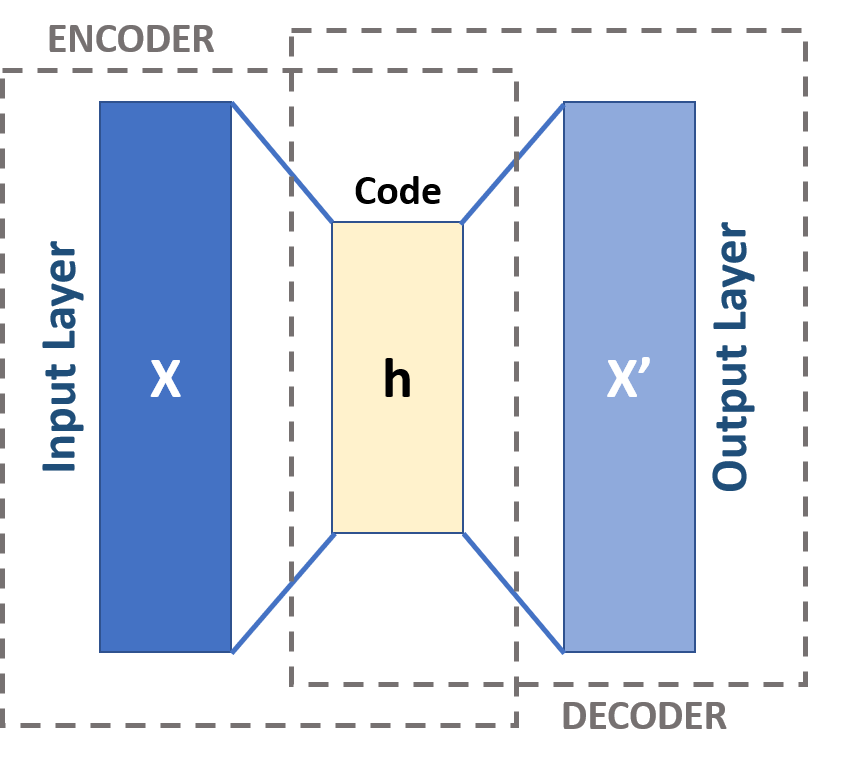
\includegraphics[width=0.50\textwidth]{images/Autoencoder_schema.png}
  \caption{The architecture of an standard autoencoder. Adapted from \url{https://upload.wikimedia.org/wikipedia/commons/3/37/Autoencoder_schema.png}}
  \label{fig:autoencoder}
\end{figure}

Typically, both $f_{\theta}$ and $g_{\phi}$ are implemented using neural network layers, often fully connected (dense) layers for tabular data or convolutional layers for image data. The activation functions used in the encoder and decoder vary by application but often include rectified linear units (ReLU) \cite{ReLU}, sigmoid, or tanh functions.

The bottleneck layer forces the model to learn the most salient features of the data by constraining the capacity of the network. This compression is critical for enabling the autoencoder to generalize rather than simply memorizing the input data.

\subsection{Training}

Training an autoencoder involves optimizing the parameters $\theta$ and $\phi$ to minimize the discrepancy between the input $\mathbf{x}$ and its reconstruction $\hat{\mathbf{x}}$. This discrepancy is typically measured using a reconstruction loss function, such as the mean squared error (MSE) for continuous data. This objective is minimized using stochastic gradient descent (SGD) or its variants such as Adam \cite{Adam}, RMSProp \cite{RMSProp}, or Adagrad \cite{Adagrad}. The gradients are computed via backpropagation, which adjusts the weights in both the encoder and decoder networks simultaneously. Proper number and size of layers, the learning rate, the loss function, and the regularization are crucial for stable and efficient training \cite{Berahmand24}.

\subsection{Variants}

Over time, numerous variants of the basic autoencoder have been proposed to overcome its limitations and enhance its representational power. One of the most influential extensions is the \textbf{denoising autoencoder} [\cite{Vincent08}, \cite{Goodfellow16}], which aims to learn robust features by reconstructing clean input from a corrupted version. By forcing the network to recover original data from noisy inputs, the model learns more meaningful representations that are invariant to small perturbations.

Another popular modification is the \textbf{sparse autoencoder}, which introduces a sparsity constraint on the latent representation. This is commonly implemented by adding a regularization term that penalizes activation levels across neurons in the bottleneck layer, encouraging the network to activate only a small subset of neurons for any given input [\cite{Ng11}, \cite{Goodfellow16}]. Such sparsity tends to produce more interpretable features and has been linked to mechanisms in biological neural systems.

A more sophisticated probabilistic framework is introduced in the \textbf{variational autoencoder (VAE)}, proposed by Kingma and Welling (2013) [\cite{Kingma13}, \cite{Bank21}]. Unlike classical autoencoders that learn a deterministic mapping to the latent space, VAEs model the latent variables as probability distributions. The encoder outputs parameters of a distribution (usually Gaussian), and the decoder generates data by sampling from this distribution. Training is achieved by maximizing the evidence lower bound (ELBO), which balances the reconstruction loss and a Kullback-Leibler (KL) divergence term that regularizes the latent distribution toward a prior, typically standard normal. This approach enables both principled generative modeling and smooth interpolation in latent space.

Further developments include \textbf{adversarial autoencoders} \cite{Makhzani16}, which incorporate an adversarial loss similar to generative adversarial networks (GANs) to shape the distribution of the latent space. Other variations include convolutional autoencoders for spatial data, recurrent or sequence-to-sequence autoencoders for temporal data, and \textbf{contractive autoencoders} that penalize the Jacobian of the encoder to enforce local invariance [\cite{Rifai11}, \cite{Goodfellow16}].

\subsection{Applications}

Autoencoders have found extensive use across a wide range of domains, owing to their ability to learn compact and informative representations of data without requiring labeled supervision. One of their earliest and most prominent applications is in \textbf{dimensionality reduction} \cite{Goodfellow16}, where they serve as nonlinear generalizations of classical techniques such as principal component analysis (PCA). While PCA can only capture linear structures, autoencoders are capable of modeling complex, nonlinear manifolds in high-dimensional input spaces \cite{Hinton06}. This capability makes them particularly effective for visualizing high-dimensional datasets such as image or genomic data, where structure and variation are not easily captured by linear projections.

Autoencoders are also widely utilized in \textbf{anomaly detection} tasks. When trained exclusively on data that are representative of a “normal” class, the model learns to reconstruct these inputs accurately. Anomalous or out-of-distribution data, which deviate significantly from the training distribution, typically result in poor reconstructions and thus higher reconstruction error [\cite{Sakurada14}, \cite{Bank21}]. This principle has been successfully applied in diverse fields including network intrusion detection, manufacturing quality assurance, and medical diagnostics.

In the realm of \textbf{denoising}, autoencoders have been used to remove noise and corruption from data. Denoising autoencoders \cite{Vincent08} are trained to recover clean inputs from deliberately perturbed versions, thereby learning noise-invariant features that generalize better to unseen data. This approach has proven especially useful in image and audio preprocessing tasks.

Another influential application of autoencoders lies in \textbf{generative modeling}. Variational autoencoders (VAEs), in particular, provide a principled probabilistic framework for generating new data samples by sampling from the learned latent distribution [\cite{Kingma13}, \cite{Bank21}]. This has led to applications in synthetic data generation, drug discovery, and creative domains such as music and art synthesis. The ability to interpolate and manipulate attributes in the latent space allows VAEs to perform meaningful transformations, such as morphing one face into another or altering specific attributes like lighting and expression.

\subsection{Limitations}

Despite their versatility, autoencoders are subject to several limitations that affect their performance and general applicability. A fundamental issue is their potential to \textbf{learn trivial identity mappings} when the architecture is unconstrained, especially if the bottleneck layer has equal or greater dimensionality than the input. In such cases, the autoencoder may merely memorize inputs without learning meaningful abstractions \cite{Goodfellow16}. This problem is mitigated by architectural constraints (such as an undercomplete representation) or regularization techniques (e.g., sparsity or noise), but it remains an inherent risk in their design.

A notable limitation of autoencoders lies in their \textbf{sensitivity to hyperparameter settings}, which can significantly affect model performance and generalizability \cite{Berahmand24}. Critical hyperparameters such as the dimensionality of the latent space, number of layers, learning rate, regularization strength, and activation functions must be carefully tuned, often through empirical trial and error or computationally expensive search procedures. Poor choices can lead to underfitting, overfitting, or convergence failures.

Another limitation concerns the \textbf{interpretability of learned features} \cite{Bengio14}. Unlike linear methods such as PCA, where each principal component can often be directly interpreted in terms of variance directions, the latent variables learned by standard autoencoders are typically entangled and lack semantic meaning. This makes it challenging to use the latent space for tasks that require transparency or explanation, such as decision support systems in healthcare.

\section{In-Between Instance}

Traditional data-mining paradigms typically categorize data points either as inliers, members of well-defined clusters, or as outliers, which deviate significantly and are often discarded. However, Kazempour et al. (2024) \cite{Kazempour24} identify a third, crucial class of elements: \textbf{in-between instances (IBIs)}. These objects do not cleanly fit into one cluster, nor do they belong to the noise category. Instead, they act as bridges, sharing properties of two or more clusters.

\subsection{Definition}

Kazempour et al. (2024) \cite{Kazempour24} formalizes in-between instances as follows: \\
\textit{Given a dataset \( X \in \mathbb{R}^{n \times d} \). Furthermore, given a partitioning $C = \{ C_1, \ldots, C_k \} \subseteq X$ and a set of outliers \( O \subseteq X \) where \( C \cap O = \emptyset \) and \( \{X\} = C \cup O \). An object \( o \in O \) is an in-between instance if it is:
\begin{itemize}
    \item[(a)] deviating mostly from the characteristics of clusters (groups) and
    \item[(b)] still exhibits some characteristics of at least two or more clusters.
\end{itemize}
This property manifests itself in the observation of an in-between instance being located between two or more clusters. Here the term \textbf{between} bares the semantic of an object being in proximity of two or more clusters, hence being potentially similar with respect to the characteristics of the clusters it is located in-between.}

Mathematically, an IBI is identified through a predicate function, or criteria, $\theta(o, C_i, C_j)$ that evaluates whether an object $o$ is in between clusters $C_i$ and $C_j$. This function is flexible and domain-specific. It may incorporate geometric properties, probabilistic affiliations, or angular relationships, depending on the chosen framework. Crucially, the IBI is not reducible to a fuzzy member of one cluster, as in soft clustering approaches, nor is it merely an outlier in the traditional sense. It occupies a third semantic and structural space that bridges categorical boundaries.

\subsection{Criteria}

Kazempour et al. (2024) \cite{Kazempour24} delineate three principal criteria, or predicate classes, by which IBIs may be recognized. Each is grounded in a different aspect of spatial or statistical analysis and is suited to different data geometries and interpretative goals.

\begin{figure}[htbp]
    \centering
    \begin{subfigure}[b]{0.475\textwidth}
        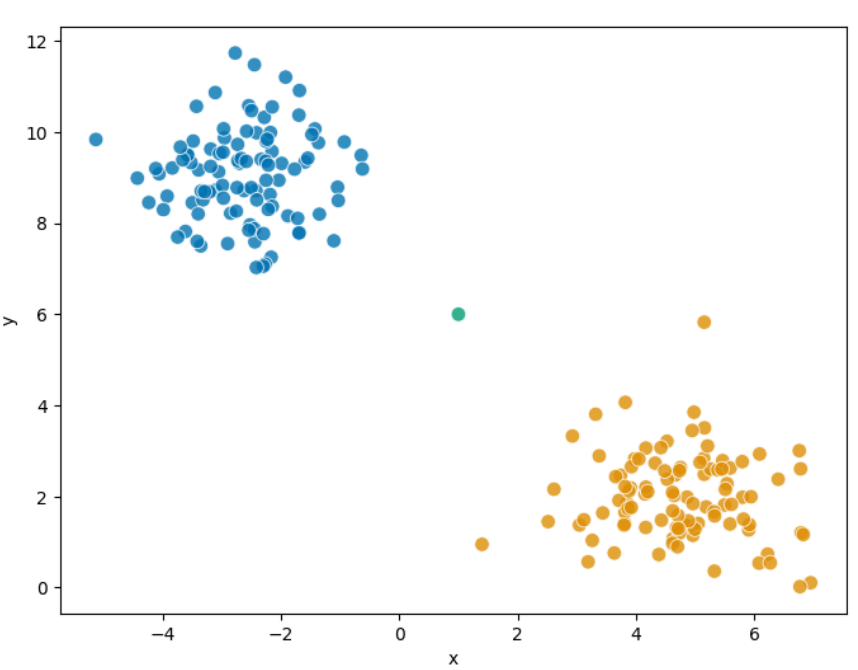
\includegraphics[width=\textwidth]{images/ibi_raw.png}
        \caption{Two clusters of data in blue and orange with an in-between instance in green.}
        \label{fig:ibi_raw}
    \end{subfigure}
    \hfill
    \begin{subfigure}[b]{0.475\textwidth}
        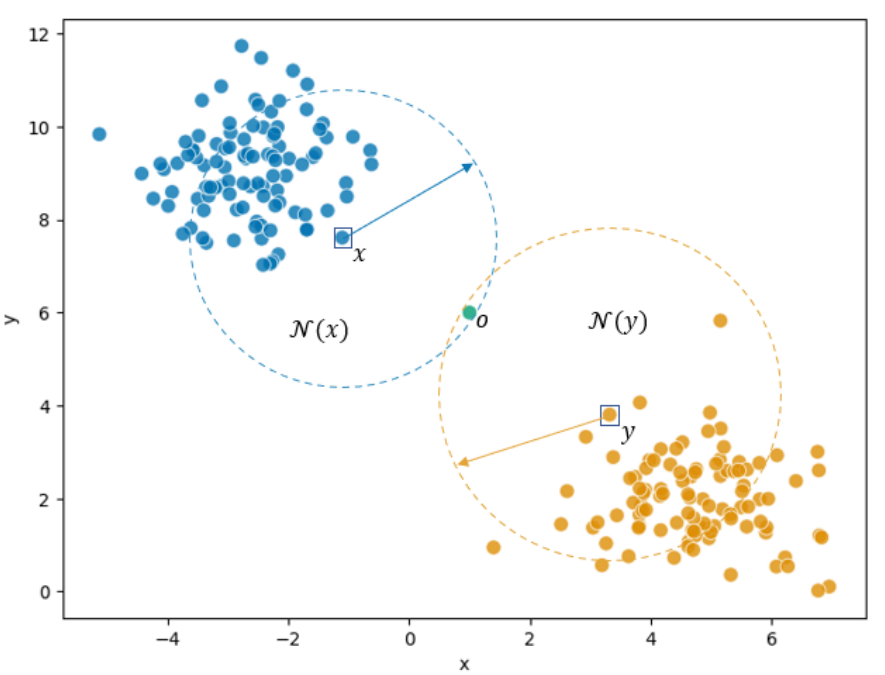
\includegraphics[width=\textwidth]{images/ibi_neighbor.png}
        \caption{Illustration of the neighborhood criterion for in-between instances.}
        \label{fig:ibi_neighbor}
    \end{subfigure}
    \vspace{0.5cm}
    \begin{subfigure}[b]{0.475\textwidth}
        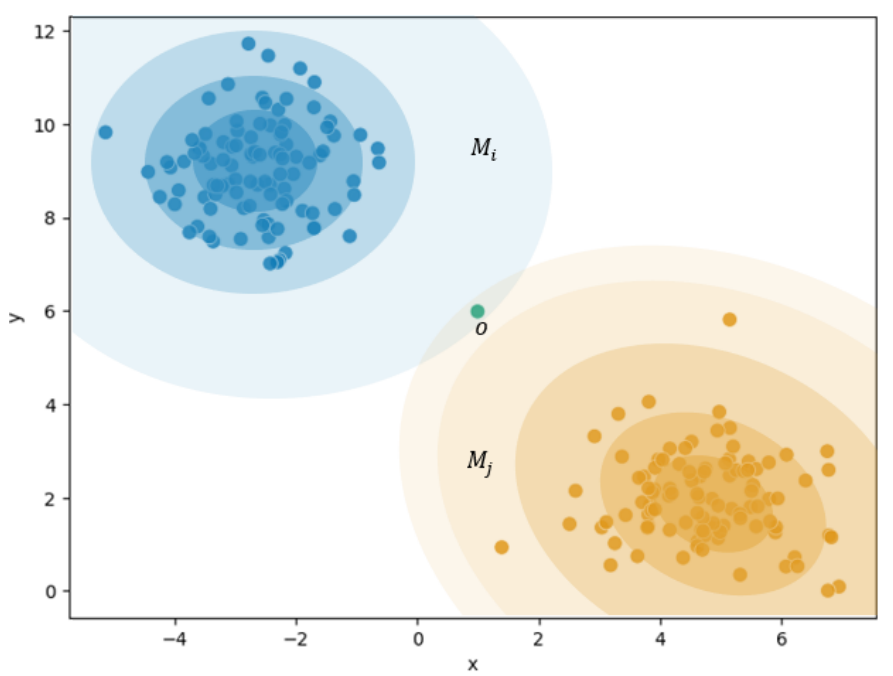
\includegraphics[width=\textwidth]{images/ibi_probability.png}
        \caption{Illustration of the class probability criterion for in-between instances.}
        \label{fig:ibi_probability}
    \end{subfigure}
    \hfill
    \begin{subfigure}[b]{0.475\textwidth}
        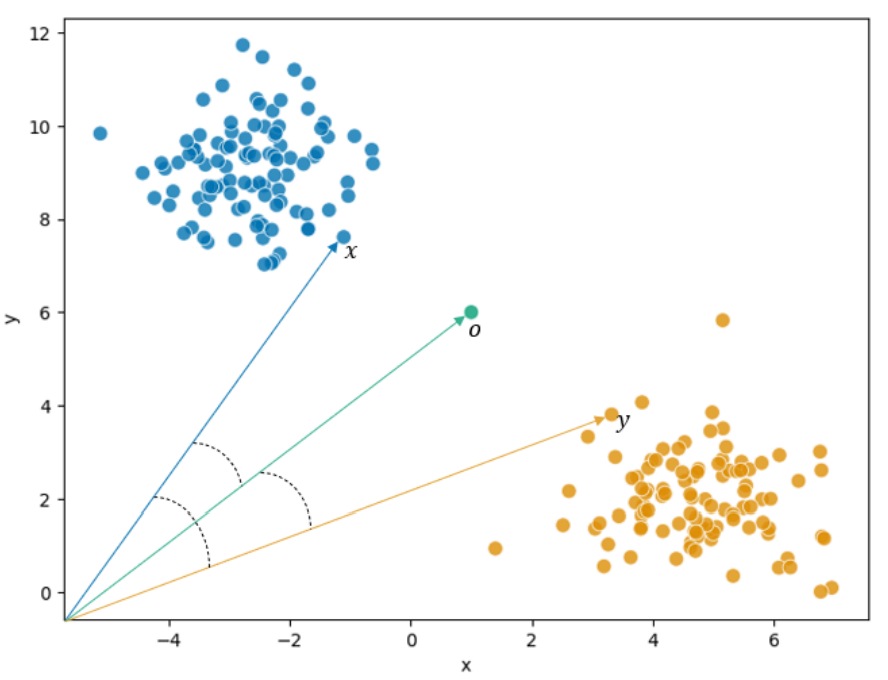
\includegraphics[width=\textwidth]{images/ibi_angle.png}
        \caption{ Illustration of the geometric criterion for in-between instances.}
        \label{fig:ibi_angle}
    \end{subfigure}
    \caption{In-between instances and its different criteria. Adapted from \cite{Kazempour24}}
    \label{fig:ibi}
\end{figure}

The \textbf{neighborhood criterion} (Figure \ref{fig:ibi_neighbor}) identifies IBIs based on local proximity. Here, an object is considered in-between if it resides within the spatial neighborhoods of at least two clusters, as determined by shared $k$-nearest neighbors or overlapping $\epsilon$-radius balls.

According to the \textbf{class probability criterion} (Figure \ref{fig:ibi_probability}), an object is an IBI if it has near-equal probabilities of belonging to at least two distinct clusters. This approach captures probabilistic ambiguity, which is especially useful in domains where uncertainty is intrinsic, such as medical diagnosis or probabilistic reasoning.

The \textbf{geometric criterion} (Figure \ref{fig:ibi_angle}) leverages vector relationships in high-dimensional space. An object is in-between if it lies directionally between representative points of two clusters. Formally, this is often framed in terms of the cosine similarity metric. An IBI, by this account, is positioned such that the angles between its vector representation and those of two cluster members are comparable, thereby confirming its intermediary status.

Each of these criteria reveals a different facet of in-betweenness and may be used independently or in combination to increase robustness and interpretability.

\subsection{Relationships to Clustering and Outlier Detection}

The concept of in-between instances reshapes traditional understandings of unsupervised learning by inserting a structurally distinct category between inliers and outliers. In classical clustering, objects are assigned to the cluster whose prototype or centroid they most closely resemble, often under assumptions of convexity or spatial separation. Outlier detection, by contrast, treats any point that deviates significantly from such groupings as anomalous, assuming it to be irrelevant noise or a rare event.

IBIs subvert this framework. They are outliers in the sense that they do not cleanly belong to any single cluster, but they are not statistical anomalies without meaning. Instead, they encode partial membership or blended features from multiple groups. This characteristic makes IBIs particularly valuable in complex, high-dimensional datasets where hybrid or transitional objects occur naturally. For example, in cultural analytics, an IBI might be a text that synthesizes themes from two distinct genres. In genomics, it might be a gene that functions across multiple pathways. In customer segmentation, an IBI could represent a consumer whose behavior aligns partially with multiple buyer personas.

Notably, IBIs are not captured by conventional clustering algorithms, including k-means \cite{kMeans} or DBSCAN \cite{DBSCAN}, nor by most standard outlier detectors like LOF (Local Outlier Factor) \cite{LOF}. These methods are not designed to detect shared affinities across cluster boundaries. Similarly, fuzzy clustering methods assign soft membership probabilities but do not explicitly highlight cases of balanced ambiguity or inter-cluster affinity. The IBI framework proposed by Kazempour et al. (2024) \cite{Kazempour24} fills this conceptual and methodological gap, proposing concepts to identify, quantify, and interpret these intermediate cases.

\newpage
\chapter{Related Work} \label{ch:related_work}

This chapter surveys the relevant literature underpinning this thesis. Reflecting the structure of the research questions posed in this thesis, the chapter is divided into three main sections. First, we examine foundational aspects of autoencoder design and the influence of architectural and hyperparameter choices. Second, we explore how various loss functions contribute to preserving the structural integrity of the data in the latent space, that is, maintaining meaningful relationships and patterns present in the original data after compression. Third, we review supervised autoencoder approaches that incorporate label information to enhance the discriminative quality of the learned embeddings. This tripartite structure provides the conceptual grounding necessary for the subsequent methods and experimental analyses.

\section{Architectures Factors of Autoencoders}

In the context of autoencoder (AE) design, understanding the architecture, hyperparameter tuning, and design principles is crucial for optimizing performance across various tasks. AEs are typically structured as artificial neural networks comprising two principal components: the encoder, which compresses the input data into a latent representation, and the decoder, which reconstructs the input from this latent code. The architectural choices and hyperparameter configurations of these networks directly influence their representational capacity, robustness, and generalization ability.

The fundamental structure of an autoencoder can vary from shallow models, with a single hidden layer acting as the bottleneck, to deep configurations that incorporate multiple hidden layers in both encoder and decoder segments. Deeper architectures are generally more expressive and capable of learning complex hierarchical representations \cite{Goodfellow16}. However, this increase in depth necessitates careful consideration of design aspects such as the choice of activation functions, weight initialization, and optimization algorithms to mitigate challenges like vanishing gradients and overfitting.

In terms of activation functions, traditional autoencoders often utilize sigmoid or tanh functions, especially in shallower networks, due to their bounded outputs and historical precedent. Nevertheless, modern deep AEs frequently adopt rectified linear units (ReLU) \cite{ReLU} and their variants, such as leaky ReLU \cite{leakyReLU} or SELU \cite{SELU}, which promote sparsity and mitigate vanishing gradient issues during training [\cite{Charte18}, \cite{Berahmand24}]. The inclusion of these activation functions often results in more efficient training dynamics and better representation quality.

The dimensionality of the bottleneck layer is a critical architectural parameter. Undercomplete autoencoders, where the latent dimension is smaller than the input, are inherently encouraged to learn compressed, informative representations. Overcomplete architectures, on the other hand, necessitate the application of additional constraints or regularization techniques, such as sparsity or noise injection, to prevent trivial identity mappings and to enforce meaningful encoding [\cite{Goodfellow16}, \cite{Charte18}].

From a hyperparameter perspective, choices such as the number of hidden units per layer, learning rate, batch size, type of optimizer, and regularization strategies significantly impact AE performance. Learning rate selection, in particular, must balance convergence speed and stability, often requiring empirical tuning. Similarly, the batch size can influence both the smoothness of gradient estimates and memory efficiency, necessitating a trade-off that is context-dependent \cite{Berahmand24}.

An additional consideration involves the selection of the loss function. Mean squared error (MSE) is a typical choice for continuous-valued data, while binary cross-entropy is preferred for binary inputs or outputs bounded within the [0,1] interval. The alignment of the loss function with the data characteristics and the overall training objective is imperative for effective learning. Furthermore, the use of advanced optimization algorithms such as Adam \cite{Adam} or RMSprop \cite{RMSProp}, which adapt learning rates for individual parameters, often facilitates more efficient training convergence, particularly in high-dimensional settings [\cite{Goodfellow16}, \cite{Charte18}, \cite{Berahmand24}].

In practical terms, AE design is an iterative and data-dependent process. While general guidelines exist, such as aligning encoder-decoder depths, mirroring layer widths, and gradually reducing the number of units toward the bottleneck, final architecture tuning often benefits from empirical validation through performance metrics \cite{Charte18}.

In summary, the design and tuning of autoencoders involve a nuanced interplay between structural decisions and hyperparameter optimization. Drawing from foundational insights by Goodfellow et al. (2016) \cite{Goodfellow16}, design strategies by Charte et al. (2018) \cite{Charte18}, and evaluations of hyperparameter sensitivity by Berahmand et al. (2024) \cite{Berahmand24}, it becomes evident that effective AE deployment hinges on a principled yet flexible approach.

\section{Loss-based Structure Preservation}

Central to the efficacy of autoencoders is the ability to preserve essential structural information in the data during reconstruction. This characteristic is typically governed by the loss function employed during training, which plays a critical role in ensuring that the encoded representation retains the salient features of the original input. The concept of loss-based structure preservation is particularly crucial when autoencoders are applied in domains where the intrinsic relationships within data must be maintained, such as financial time series forecasting \cite{Bieganowski24}.

A conventional autoencoder consists of an encoder that maps input data to a lower-dimensional latent space and a decoder that reconstructs the input from this compressed representation. The optimization of this process is generally driven by a reconstruction loss, often measured using metrics like mean squared error (MSE) or binary cross-entropy, depending on the nature of the input data. While such basic losses encourage fidelity between the input and its reconstruction, they do not inherently preserve the geometric or topological structure of the input space. Consequently, researchers have extended traditional autoencoder models to incorporate loss terms explicitly designed to preserve local and global structures in the data \cite{Goodfellow16}.

One of the earliest and most influential approaches to incorporating structural information into the autoencoder's loss function is the use of contractive autoencoders, which penalize the Jacobian of the encoder’s output with respect to its input. This method enforces the learned representation to be locally invariant to small perturbations in the input space, thereby preserving local structure \cite{Rifai11}.

The idea of structure preservation has been further refined in manifold learning-inspired variants such as the locally linear embedding (LLE) autoencoder. These models integrate principles from classical manifold learning into the loss function by penalizing discrepancies in local neighborhood relationships between the original data and the latent representations. For example, the Laplacian autoencoder incorporates a graph Laplacian regularization term into the loss function, promoting the preservation of the graph structure induced by nearest-neighbor relationships in the input space [\cite{Miani22}, \cite{Wang14}]. This encourages the autoencoder to maintain local isometry, ensuring that similar inputs remain close in the latent space.

In addition to preserving local structures, several works have focused on global structural preservation, particularly when the autoencoder is applied to data with hierarchical or graph-based relationships. Graph autoencoders, for instance, are designed to learn node embeddings that reflect the structure of the graph, often using reconstruction losses that penalize errors in predicting adjacency relationships or graph Laplacian properties \cite{Kipf16}. These models demonstrate how loss functions can be adapted to handle more complex relational structures, expanding the applicability of autoencoders beyond grid-structured data to network-structured inputs.

The challenge of preserving structure becomes more pronounced in variational autoencoders (VAEs), where the probabilistic nature of the latent space can lead to more diffuse representations. To counteract this, researchers have proposed various modifications to the VAE objective, such as the $\beta$-VAE, which introduces a weighting factor on the Kullback-Leibler divergence term to control the trade-off between reconstruction accuracy and latent space disentanglement \cite{Burgess18}.

In addition to conventional structure-preserving strategies, equipping autoencoders with specialized loss functions tailored for clustering tasks has become an increasingly effective approach to bridge the gap between representation learning and clustering tasks. Classic autoencoders trained solely on reconstruction loss often produce latent spaces that are not inherently conducive to clustering, as they optimize for data fidelity rather than cluster separability. To address this, researchers have developed clustering-specific loss functions that can be incorporated into the training regime of autoencoders to promote latent space organization aligned with clustering objectives [\cite{Leiber25}, \cite{Beer24}].

In summary, the loss-based preservation of structure in autoencoders represents a broad and evolving research area. The design of loss functions that go beyond simple reconstruction error is critical to ensuring that autoencoders produce meaningful and structurally coherent representations. Whether through local neighborhood preservation, graph-based constraints, contrastive objectives, or probabilistic regularization, these approaches collectively aim to align the latent representations with the intrinsic geometry and semantics of the input space. As such, the ongoing refinement of loss functions tailored to structure preservation continues to be a key driver in the advancement of autoencoder architectures and their applications across diverse domains.

\section{Supervised Autoencoders}

Supervised autoencoders represent a sophisticated integration of unsupervised and supervised learning paradigms, combining the representational power of traditional autoencoders with the predictive capabilities of supervised models. While conventional autoencoders are designed to learn efficient low-dimensional representations of data through the task of reconstructing input signals, supervised autoencoders extend this framework by incorporating label information into the learning process. This fusion enables the latent representations to be not only compact and informative but also discriminative with respect to specific supervised objectives \cite{Le18}.

Training a supervised autoencoder involves optimizing a composite loss function that typically includes a reconstruction loss, such as the mean squared error, and a supervised loss. This dual-objective optimization forces the model to balance between reconstructing the input accurately and producing latent features conducive to accurate predictions \cite{Le18}.

One of the key advantages of supervised autoencoders lies in their ability to learn task-specific representations that are more aligned with the predictive objective than those learned by purely unsupervised methods. In many domains, such as medical imaging \cite{Rajpurkar17}, natural language processing \cite{Devlin18}, object detection \cite{Ren16} and time series forecasting \cite{Bieganowski24} incorporating label information during representation learning has been shown to improve downstream performance.

Despite their advantages, supervised autoencoders are not without limitations. One common concern is the potential for the supervised loss to dominate training, leading to latent representations that are highly predictive but lack generative capacity or robustness to noise \cite{Le18}.

A prevalent strategy within supervised autoencoders is the use of metric learning, particularly through the incorporation of triplet loss. This approach has been successfully demonstrated in models like the Triplet Enhanced AutoEncoder (TEA), which reformulates label information as triplets, comprising an anchor, a positive sample from the same class, and a negative sample from a different class, to guide the embedding process. By enforcing that the anchor is closer to the positive than to the negative in the latent space, the model achieves a latent structure that preserves both network topology and class separability without being tied to a specific classifier, a property referred to as being model-free \cite{Yang19}.

Triplet-based supervision has also been extended to generative frameworks such as the Triplet Variational Autoencoder (TVAE). In this approach, the triplet loss is jointly optimized with the Evidence Lower Bound (ELBO) of the VAE, effectively combining reconstruction fidelity, latent regularization, and metric learning to yield more discriminative embeddings. Empirical results indicate that such a hybrid loss structure significantly improves triplet accuracy compared to traditional VAEs \cite{Ishfaq23}.

Beyond triplet loss, other supervised strategies have been proposed to enhance autoencoder-based representation learning. The Supervised COSMOS Autoencoder, for instance, incorporates a multi-objective loss function comprising cosine similarity, Mahalanobis distance, and a mutual information-based supervision term. This architecture is designed to capture both angular and statistical relationships in the data while explicitly promoting class discriminability. The model demonstrates that incorporating supervision can lead to latent spaces that are not only robust to input variations such as illumination and pose but also better aligned with classification objectives \cite{Singh18}.

In summary, supervised autoencoders provide a compelling framework for learning representations that are simultaneously compact, interpretable, and predictive. By integrating supervised objectives into the autoencoding process, these models offer a principled way to incorporate domain knowledge and task-specific signals into representation learning. Their flexibility and adaptability have made them an increasingly popular choice across a wide range of machine learning applications, and ongoing research continues to refine their architectures, training procedures, and theoretical underpinnings.

\section{The Research Gap}

The reviewed literature highlights the crucial influence of both architectural configurations and loss functions on the ability of autoencoders to preserve meaningful structural relationships within data. While prior work has proposed various advanced architectures and structure-aware loss formulations, a systematic investigation into their impact on the preservation of in-between instances (IBIs) remains absent. Building upon these insights, this thesis adopts an experimental approach that evaluates the effects of key architectural choices and loss strategies on IBI preservation.
\newpage
\chapter{Method} \label{ch:method}

This chapter outlines the methodological approach used to evaluate how different autoencoder architectures and loss functions affect the preservation of in-between instances (IBIs). It details the design of synthetic datasets, the structure and training of the autoencoder models, the implementation of various loss functions and the evaluation strategies used to assess representational quality.

\section{Datasets}

\begin{table}[h]
\centering
\renewcommand{\arraystretch}{1.5} % More row height
\begin{tabular}{|
  >{\centering\arraybackslash}m{3.25cm} |
  >{\centering\arraybackslash}m{1.25cm} |
  >{\centering\arraybackslash}m{1.50cm} |
  >{\centering\arraybackslash}m{1.25cm} |
  >{\centering\arraybackslash}m{2.75cm} |}
\hline
\textbf{Name} & \textbf{Dim.} & \textbf{Points} & \textbf{IBIs} & \textbf{Clusters} \\
\hline
\textbf{2DBlobsS}    & 2D & 153 & 3   & 3 Blobs     \\
\textbf{2DBlobsM}    & 2D & 154 & 2+2 & 3 Blobs     \\
\textbf{2DMoons}     & 2D & 101 & 1   & 2 Moons     \\
\textbf{2DSwissRoll} & 2D & 202 & 1+1 & 1 SwissRoll \\
\hline
\textbf{3DBlobsS}    & 3D & 228 & 3   & 3 Blobs     \\
\textbf{3DBlobsM}    & 3D & 229 & 2+2 & 3 Blobs     \\
\textbf{3DMoons}     & 3D & 302 & 2   & 2 Moons     \\
\textbf{3DSwissRoll} & 3D & 404 & 2+2 & 1 SwissRoll \\
\textbf{3DTorus}     & 3D & 402 & 2   & 2 Tori      \\
\textbf{3DSphere}    & 3D & 492 & 2+2 & 3 Spheres   \\
\hline
\end{tabular}
\caption{Overview of synthetic datasets used in the study, categorized by dimensionality (2D or 3D). Each dataset is described by its number of points/instances, the number of in-between instances (IBIs), and the count and type of clusters present.}
\label{tab:datasets}
\end{table}

In this study, only synthetic datasets (Table \ref{tab:datasets}) are employed, as real-world datasets containing explicitly labeled in-between instances (IBIs) are, due to the novelty of the task itself, difficult to obtain. In some cases, sections of clusters are assigned different colors to enhance visual interpretability in subsequent analyses. However, these color-coded segments are not treated as separate clusters in the experimental evaluation, and IBIs themselves are not considered part of any cluster. The datasets are designed to encompass a variety of cluster configurations, including both simple and complex geometries, in order to capture a broad spectrum of spatial relationships and manifold structures. Furthermore, they vary in the number of instances, the density of clusters, and the degree of inter-cluster separation, thereby providing a diverse set of scenarios for systematically assessing model performance under differing structural complexities.
\newline

\newlength{\myimgwidth}
\setlength{\myimgwidth}{0.40\textwidth}

\begin{wrapfigure}{r}{\myimgwidth}
    \centering
    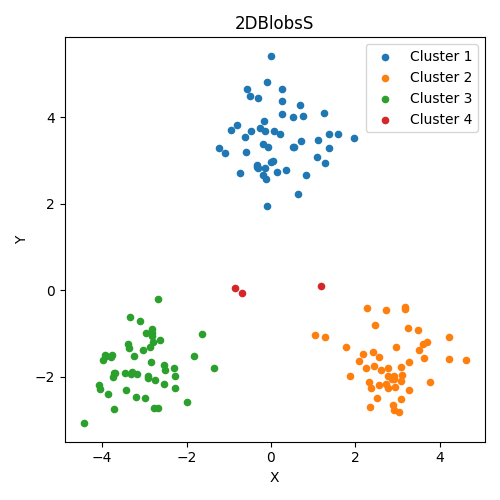
\includegraphics[width=\myimgwidth]{images/datasets/2DBlobsS.png}
    \caption{2DBlobsS.}
    \label{fig:2DBlobsS}
\end{wrapfigure}
The \textbf{2DBlobsS} dataset (Figure \ref{fig:2DBlobsS}) is a synthetic two-dimensional dataset consisting of three compact Gaussian clusters (blue, orange, and green) with no overlap. Each cluster contains densely concentrated points surrounding a central mean. Two additional points (red) are positioned between the clusters and are labeled as in-between instances (IBIs). These IBIs occupy intermediate positions in the feature space, capturing structural transitions between distinct clusters. The clear separation between clusters make this dataset a simple, low-complexity scenario for evaluating structure preservation in learned embeddings.
\newline

\begin{wrapfigure}{l}{\myimgwidth}
    \centering
    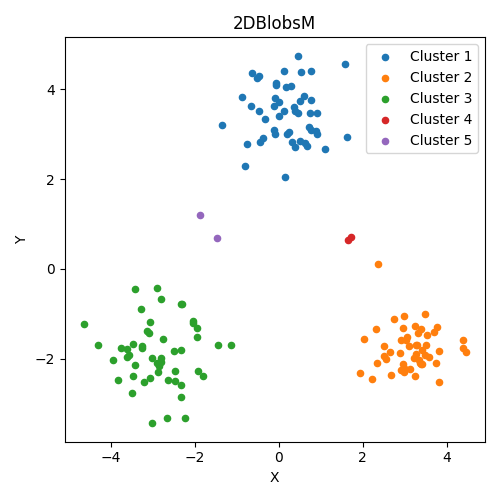
\includegraphics[width=\myimgwidth]{images/datasets/2DBlobsM.png}
    \caption{2DBlobsM.}
    \label{fig:2DBlobsM}
\end{wrapfigure}
The \textbf{2DBlobsM} dataset (Figure \ref{fig:2DBlobsM}) is a synthetic two-dimensional dataset composed of three primary Gaussian clusters, each depicted in a distinct color (blue, orange, and green). These clusters contain tightly grouped data points distributed around separate centroids. In addition to the main clusters, there are two pairs of points (red and purple) located between the clusters. These points are designated as in-between instances (IBIs), approximately equidistant from two clusters. This spatial configuration makes the dataset suitable for testing the ability to preserve both cluster integrity and multiple transitional relationships in the latent space.
\newline
\newpage

\begin{wrapfigure}{r}{\myimgwidth}
    \centering
    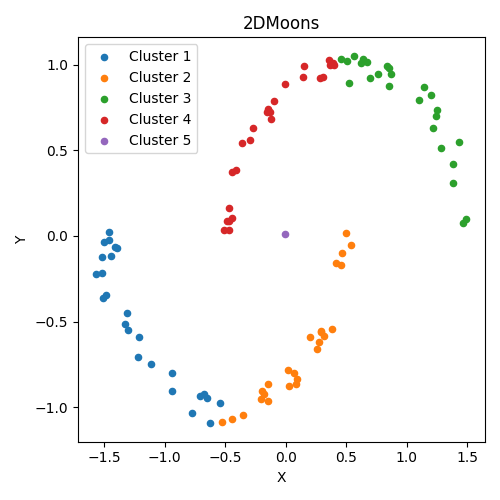
\includegraphics[width=\myimgwidth]{images/datasets/2DMoons.png}
    \caption{2DMoons.}
    \label{fig:2DMoons}
\end{wrapfigure}
The \textbf{2DMoons} dataset (Figure \ref{fig:2DMoons}) is a synthetic two-dimensional dataset composed of two interleaving half-moon–shaped clusters arranged in a nonlinear configuration. Each cluster is subdivided into two labeled segments (blue–orange and green–red) to facilitate analysis of local structure. A single point (purple) is located between the arcs and designated as an in-between instance (IBI), meaning it shares spatial proximity to both curved manifolds. The dataset’s non-linear topology and minimal number of IBIs make it a challenging case for dimensionality reduction methods that aim to preserve both manifold geometry and transitional points.
\newline

\begin{wrapfigure}{l}{\myimgwidth}
    \centering
    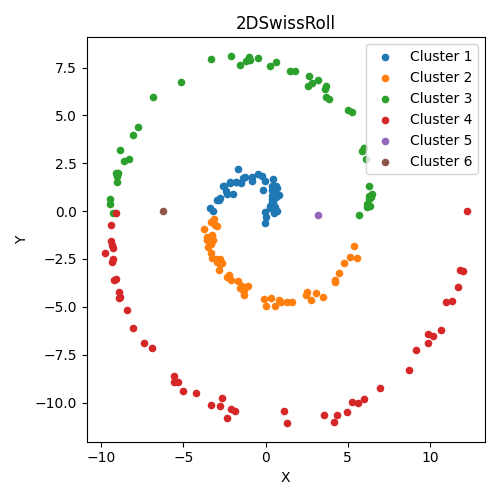
\includegraphics[width=\myimgwidth]{images/datasets/2DSwissRoll.png}
    \caption{2DSwissRoll.}
    \label{fig:2DSwissRoll}
\end{wrapfigure}
The \textbf{2DSwissRoll} dataset (Figure \ref{fig:2DSwissRoll}) is a synthetic two-dimensional dataset representing an rolled spiral manifold. The continuous spiral is segmented into contiguous curved sections (blue, orange, green, and red). Additional points (purple and brown) are placed between the main clusters and are labeled as in-between instances (IBIs). These IBIs lie along the spiral arms where neighboring sections meet, capturing transitional regions in the manifold’s geometry. The dataset’s continuous but highly non-linear structure makes it a strong benchmark for evaluating the ability to maintain neighborhood relationships and inter-cluster continuity.
\newline

\begin{wrapfigure}{r}{\myimgwidth}
    \centering
    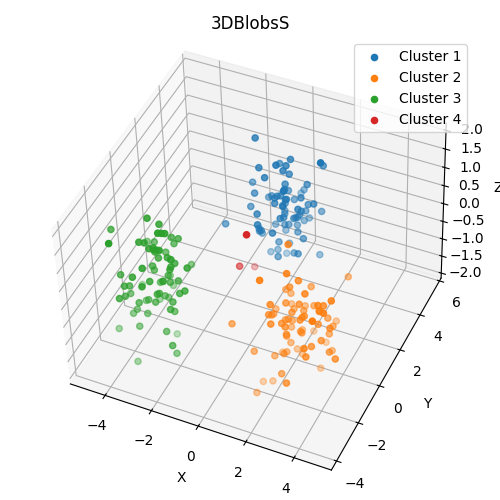
\includegraphics[width=\myimgwidth]{images/datasets/3DBlobsS.png}
    \caption{3DBlobsS.}
    \label{fig:3DBlobsS}
\end{wrapfigure}
The \textbf{3DBlobsS} dataset (Figure \ref{fig:3DBlobsS}) is a synthetic three-dimensional dataset composed of three compact Gaussian clusters (blue, orange, and green) arranged with no spatial overlap. Three additional points (red) are placed between the primary clusters and are labeled as in-between instances (IBIs). These IBIs represent transitional samples that capture mixed characteristics from all clusters. The dataset’s relatively simple structure, low number of IBIs, and well-separated clusters provide a controlled environment for testing structure preservation and neighborhood fidelity.
\newline

\begin{wrapfigure}{l}{\myimgwidth}
    \centering
    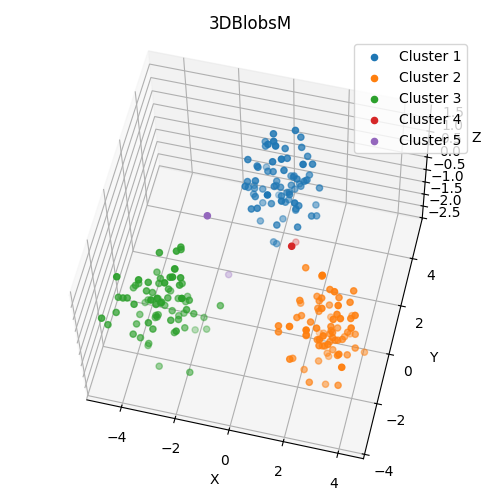
\includegraphics[width=\myimgwidth]{images/datasets/3DBlobsM.png}
    \caption{3DBlobsM.}
    \label{fig:3DBlobsM}
\end{wrapfigure}
The \textbf{3DBlobsM} dataset (Figure \ref{fig:3DBlobsM}) is a synthetic three-dimensional dataset generated from Gaussian distributions. It contains three main clusters (blue, orange, and green), each centered at distinct locations in the feature space. Two additional pairs of points (red and purple) are positioned in regions between the clusters and are designated as in-between instances (IBIs). These IBIs are situated approximately equidistant from multiple cluster centroids, forming transitional data points that share attributes of more two clusters. The dataset’s moderate complexity makes it suitable for evaluating how well the models preserve both distinct cluster boundaries and transitional relationships in low-dimensional embeddings.
\newline

\begin{wrapfigure}{r}{\myimgwidth}
    \centering
    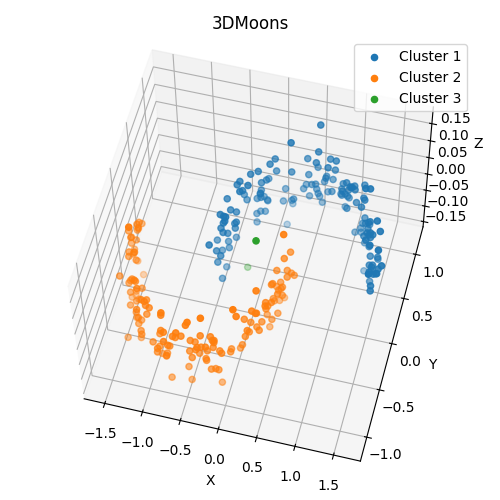
\includegraphics[width=\myimgwidth]{images/datasets/3DMoons.png}
    \caption{3DMoons.}
    \label{fig:3DMoons}
\end{wrapfigure}
The \textbf{3DMoons} dataset (Figure \ref{fig:3DMoons}) is a synthetic three-dimensional dataset characterized by two moon-shaped clusters (blue and orange). A single point (green) is placed between the two moons and labeled as an in-between instance (IBI). This IBI occupies a region of balanced proximity to both moons, representing a transitional point between distinct curved manifolds. The dataset’s non-linear geometry, combined with its minimal number of IBIs, makes it an effective benchmark for testing the ability to capture manifold structure and preserve transitional instances.
\newline

\begin{wrapfigure}{l}{\myimgwidth}
    \centering
    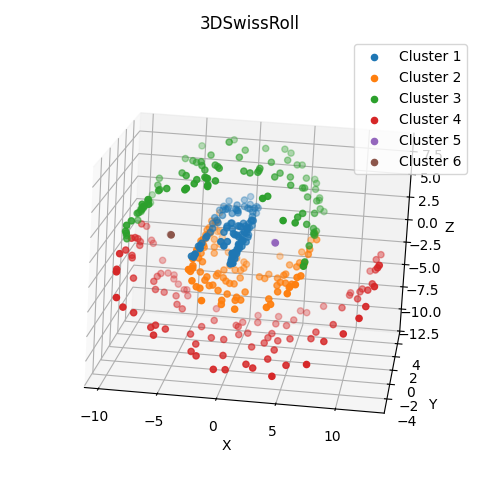
\includegraphics[width=\myimgwidth]{images/datasets/3DSwissRoll.png}
    \caption{3DSwissRoll.}
    \label{fig:3DSwissRoll}
\end{wrapfigure}
The \textbf{3DSwissRoll} dataset (Figure \ref{fig:3DSwissRoll}) is a synthetic three-dimensional dataset shaped as a rolled spiral manifold embedded in 3D space. The spiral is segmented into contiguous curved sections (blue, orange, green, and red). Several points (purple and brown) are positioned at boundary regions between clusters and are labeled as in-between instances (IBIs). These IBIs lie in areas where the manifold’s continuity creates local proximity between points from different labeled sections. The dataset’s highly non-linear geometry and mixed local–global proximity relationships make it a challenging benchmark for assessing neighborhood preservation and inter-cluster continuity.
\newline

\begin{wrapfigure}{r}{\myimgwidth}
    \centering
    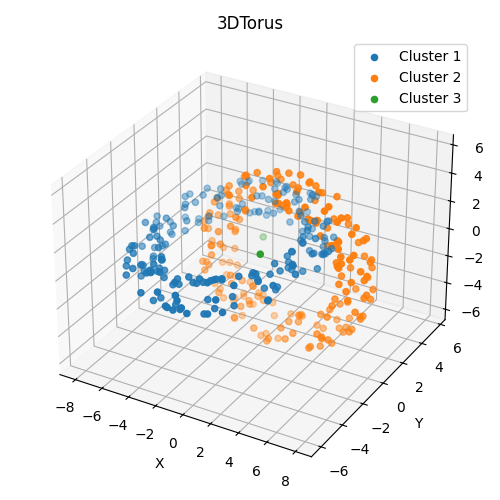
\includegraphics[width=\myimgwidth]{images/datasets/3DTorus.png}
    \caption{3DTorus.}
    \label{fig:3DTorus}
\end{wrapfigure}
The \textbf{3DTorus} dataset (Figure \ref{fig:3DTorus}) is a synthetic three-dimensional dataset featuring two ring-shaped clusters (blue and orange) arranged in a toroidal configuration. The rings are positioned in parallel, forming a closed-loop geometry. Two points (green) are placed between the two rings and designated as an in-between instance (IBI). This IBI represents a transitional sample that resides between distinct curved manifolds within the torus structure. The dataset’s global circular topology and localized inter-ring relationships make it suitable for testing the ability of embedding methods to preserve both geometric structure and transitional regions.
\newline

\begin{wrapfigure}{l}{\myimgwidth}
    \centering
    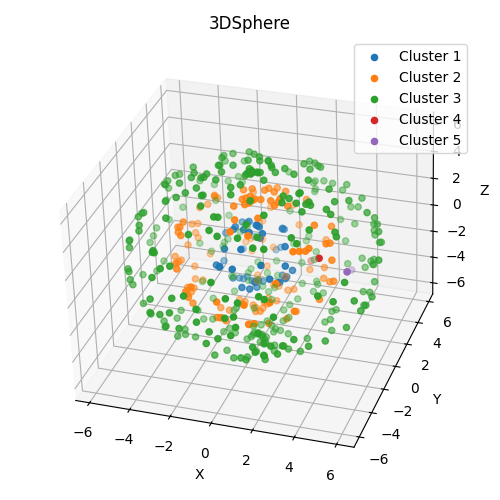
\includegraphics[width=\myimgwidth]{images/datasets/3DSphere.png}
    \caption{3DSphere.}
    \label{fig:3DSphere}
\end{wrapfigure}
The \textbf{3DSphere} dataset (Figure \ref{fig:3DSphere}) is a synthetic three-dimensional dataset consisting of three spherical clusters (blue, orange, and green) arranged as nested shells around a central origin. Points are uniformly distributed across each spherical surface. Additional points (red and purple) are positioned between these spherical shells and labeled as in-between instances (IBIs). These IBIs represent transitional samples located in intermediate radial zones, sharing spatial characteristics with multiple spherical layers. The dataset’s symmetric, non-linear geometry provides a robust test for evaluating global shape preservation and the accurate mapping of transitional points in reduced-dimensional representations.

\section{Autoencoder Framework} \label{sec:autoencoder_framework}

The framework of the autoencoders investigated in this thesis is structured around three central components, as outlined in Figure \ref{fig:roadmap}: architectural design, training stategy and loss configuration. These elements form the foundation for investigating how autoencoders can effectively capture in-between instances (IBIs) in high-dimensional data. While several hyperparameters are varied during experimentation, others are kept constant throughout. This setup provides a controlled yet flexible framework for assessing the impact of architectural and loss design choices. Each of these components is described in detail in the following sections.
\begin{figure}[ht]
    \centering
    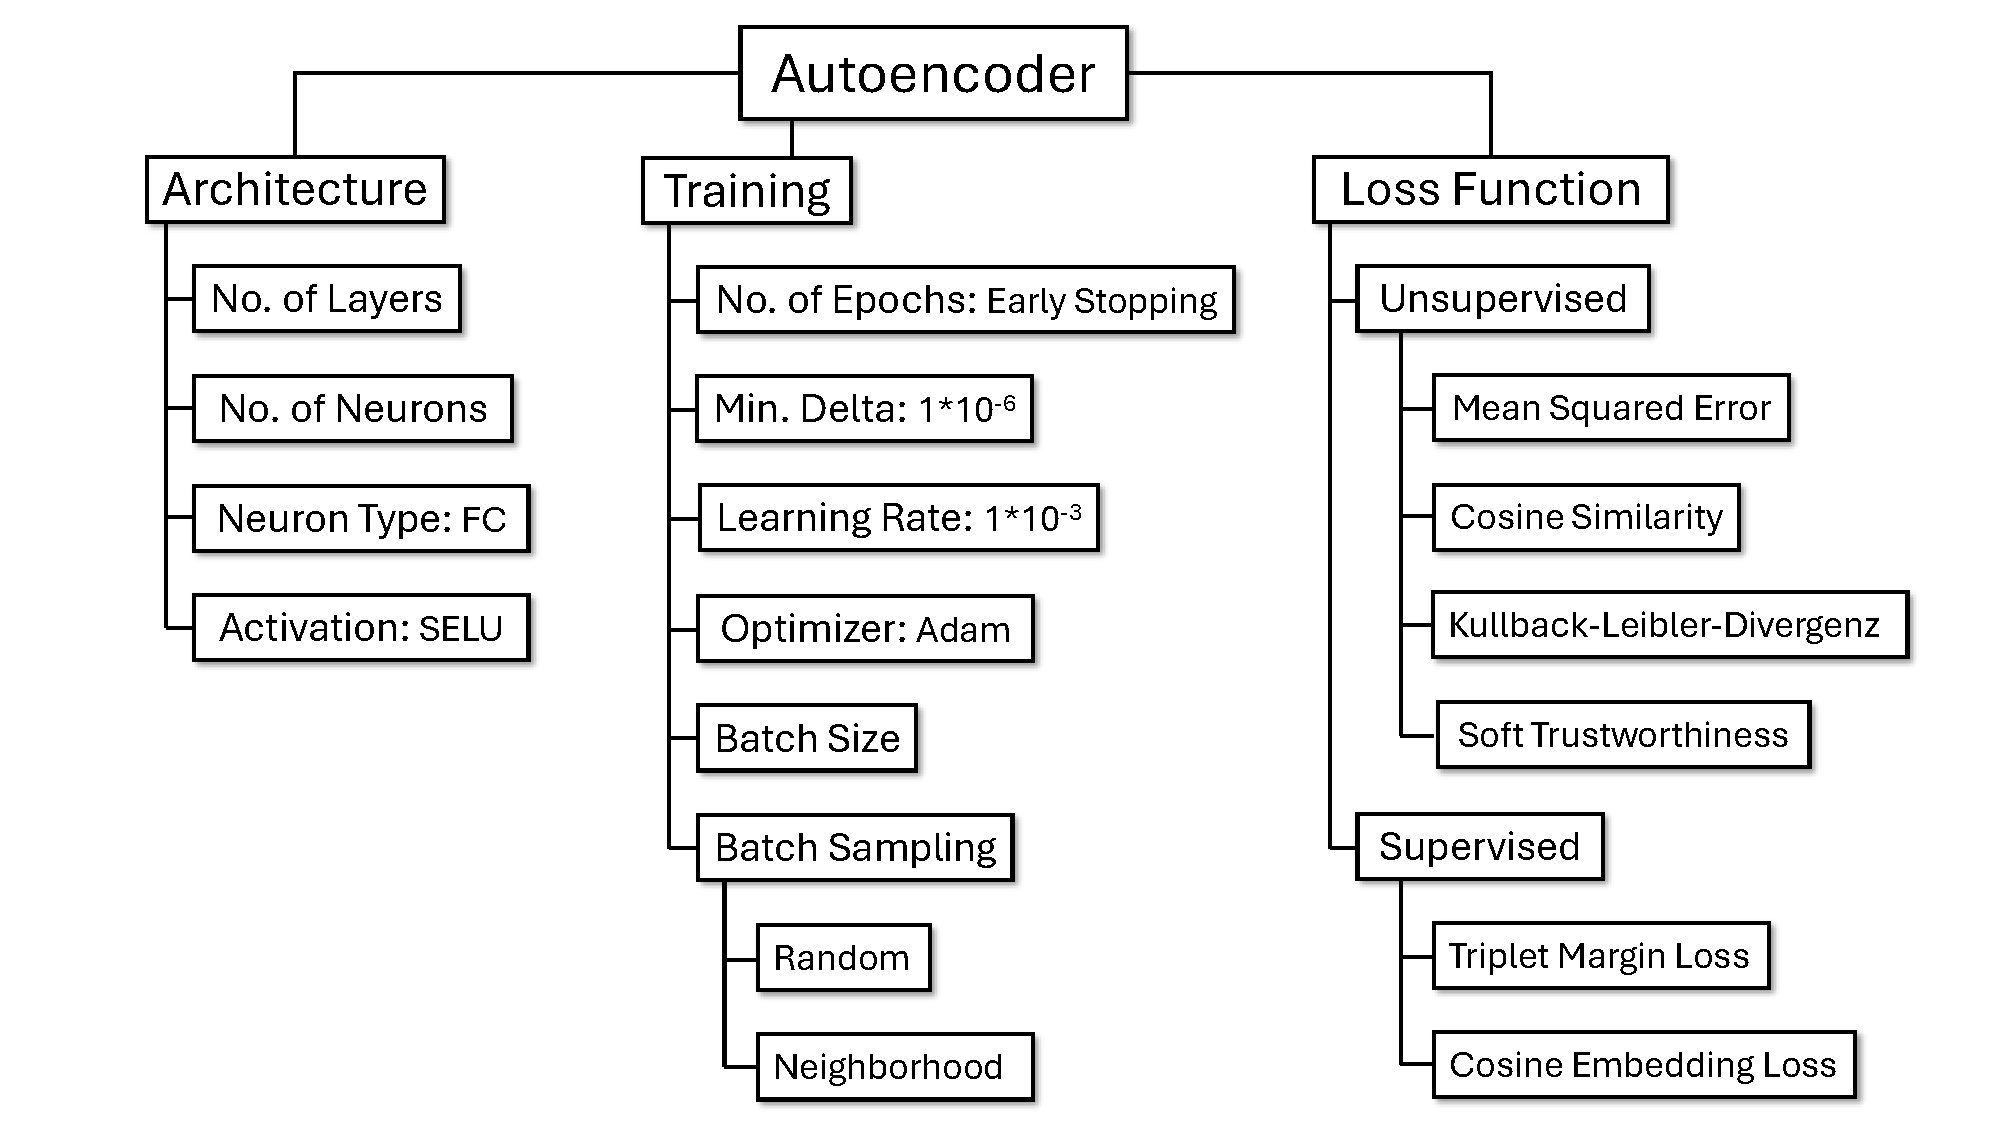
\includegraphics[width=\linewidth]{images/Roadmap.pdf}
    \caption{Overview of the framework, illustrating the three core components that guide the experimental design. Constant parameters are indicated accordingly. Inspired by \cite{Charte18}}
    \label{fig:roadmap}
\end{figure}

\subsection{Architecture and Training Strategy}

The performance and representational capacity of autoencoders are profoundly influenced by the architectural choices and training configurations employed during model development. This section outlines the specific design decisions made in constructing the autoencoder models used in this thesis. Additionally, it details key training parameters that directly impact the model’s convergence behavior and generalizability. Each choice is grounded in both theoretical considerations and empirical best practices, ensuring that the resulting autoencoder configurations are well-suited to capturing in-between instances (IBIs) while maintaining reconstruction fidelity and training stability.

\paragraph{Number of Epochs:} The number of epochs refers to the number of complete passes through the entire training dataset during the learning process. Selecting an appropriate number of epochs is critical, as it directly influences model performance and generalization. If the number of epochs is too low, the model may underfit, failing to capture meaningful patterns in the data. If too high, it risks overfitting, learning noise rather than underlying structure \cite{Berahmand24}. To mitigate this, all experiments will employ early stopping, a regularization technique that halts training when the validation performance ceases to improve beyond a defined threshold. Specifically, a minimum delta value of $1\cdot10^{-5}$ will be used to determine the smallest improvement in validation loss considered significant. If the improvement falls below this threshold for a set number of epochs, training is terminated early. This approach ensures a balanced training process, promoting both efficiency and generalizability across different configurations and datasets.

\paragraph{Neuron Type:} Neuron types vary based on the specific computational roles they fulfill. Fully connected neurons, fundamental to traditional multilayer perceptrons, are characterized by each neuron in one layer being connected to every neuron in the subsequent layer, allowing for rich, but often computationally intensive, interactions across the network. Convolutional neurons are structured to exploit spatial hierarchies by processing data through localized receptive fields using shared weights, making them particularly effective for image and pattern recognition tasks. Recurrent neurons introduce a temporal dimension by incorporating feedback loops that allow information to persist across time steps, enabling the modeling of sequential data such as language or time series [\cite{Berahmand24}, \cite{Charte18}]. However, for all experiments in this study, we exclusively employ fully connected neurons, as our data does not involve sequential or image-based features and thus does not require the specialized processing capabilities of convolutional or recurrent architectures.

\paragraph{Learning Rate:} The learning rate is a critical hyperparameter that governs the magnitude of weight updates during training, directly influencing the speed and stability of the optimization process. It determines how much the model's parameters are adjusted in response to the calculated error from each iteration of backpropagation. A learning rate that is too high can cause the model to overshoot minima in the loss landscape, potentially leading to divergence or oscillation rather than convergence. Conversely, a learning rate that is too low may result in excessively slow training and an increased risk of becoming trapped in local minima or saddle points. Adaptive optimization algorithms, dynamically adjust the rate during training to balance convergence speed with stability [\cite{Berahmand24}, \cite{Charte18}]. In our experiments the initial learning rate is set to $1\cdot10^{-3}$.

\paragraph{Optimization Algorithm:} Optimization algorithms are fundamental to training machine learning models, as they govern how model parameters are updated to minimize a loss function. Stochastic Gradient Descent (SGD) is one of the simplest and most widely used optimization methods. It updates parameters by computing the gradient of the loss with respect to the parameters using a randomly selected subset of data, introducing noise that can help escape local minima. However, SGD can be inefficient, especially in scenarios involving sparse data or ill-conditioned loss landscapes. To address such limitations, adaptive learning rate methods have been developed. AdaGrad \cite{Adagrad}, for instance, adapts the learning rate for each parameter individually by accumulating the square of past gradients, which improves performance on sparse data but can lead to overly small learning rates over time. RMSProp \cite{RMSProp} modifies AdaGrad by using an exponentially decaying average of squared gradients, preventing the learning rate from diminishing too quickly and thereby maintaining consistent progress. Building upon both RMSProp and momentum-based updates, Adam (Adaptive Moment Estimation) \cite{Adam} computes adaptive learning rates using estimates of the first and second moments of the gradients \cite{Berahmand24}. By combining the benefits of RMSProp and momentum, Adam tends to perform robustly across a wide range of deep learning tasks \cite{Charte18}. Due to its efficiency and strong empirical performance, we will employ the Adam optimizer in all our experiments.

\paragraph{Batch Size:} The batch size, the number of samples processed before updating model parameters, significantly influences both training efficiency and model performance. Smaller batch sizes result in more frequent updates, which can help the model escape local minima, potentially enhancing generalization. However, these frequent updates introduce greater noise into the gradient estimates, which may destabilize training and slow overall progress. In contrast, larger batch sizes yield more stable and accurate gradient estimates, enabling faster convergence, though they demand more memory. Selecting an optimal batch size is highly context-dependent, influenced by the model architecture, dataset characteristics, and hardware constraints \cite{Berahmand24}. Consequently, in this work, the batch size will be treated as a variable hyperparameter, systematically varied and tested across experiments to assess its impact on training dynamics and generalization performance.

\paragraph{Batch Sampling:} Batch sampling refers to the process of selecting subsets of data points from the full training dataset to compute gradients and update model parameters during training. Traditionally, batches are sampled randomly, ensuring that each mini-batch represents a diverse mix of the data distribution, which helps improve generalization \cite{LeCun12}. However, alternative strategies like neighborhood sampling have gained attention, particularly in domains such as graph neural networks \cite{Hamilton18}, where local context plays a significant role. Neighborhood sampling involves selecting data points that are close to each other in some feature space or topological structure, thereby preserving local correlations and potentially enhancing learning from structured or spatially coherent data. The choice between random and neighborhood sampling is not arbitrary and should be informed by the nature of the loss function used in the experiments. If the loss is global, aggregating information across the entire dataset, random sampling is generally more appropriate. In contrast, if the loss function emphasizes local patterns or relationships, neighborhood sampling can provide more relevant gradient updates. Thus, sampling strategy must be aligned with the scope of the loss function to optimize learning efficacy.

\paragraph{Activation Function:} Activation functions (Table \ref{tab:activations_functions}) are a critical component in artificial neural networks, including autoencoders, where they endow the model with the capacity to capture and learn complex, non-linear relationships in data. These functions operate by transforming the weighted sum of inputs into a node’s output, introducing non-linearity into the model’s computations. Without them, a network composed of only linear operations would be functionally equivalent to a linear model. Among the most commonly used activation functions in autoencoders are the sigmoid and hyperbolic tangent (tanh), both of which are bounded. The sigmoid maps input values to the range [0, 1], while tanh spans [-1, 1], often resulting in stronger gradients and better convergence \cite{Berahmand24}. Rectified Linear Units (ReLU) \cite{ReLU} are also widely used due to their simplicity, although their tendency to output zero for negative inputs can hinder the reconstruction performance in some autoencoder configurations \cite{Charte18}. To address this, more advanced variants like the Scaled Exponential Linear Unit (SELU) \cite{SELU} have been developed, which can maintain a healthy flow of gradients. Given SELU’s benefits, we will therefore be using it as the activation function in our experiments to enhance the reconstruction fidelity.

\begin{table}[ht]
\centering
\renewcommand{\arraystretch}{1.5} % More row height
\begin{tabular}{|
  >{\centering\arraybackslash}m{3cm} |
  >{\centering\arraybackslash}m{5cm} |
  >{\centering\arraybackslash}m{1.33cm} |
  >{\centering\arraybackslash}m{4cm} |}
\hline
\textbf{Name} & \textbf{Equation} & \textbf{Output} & \textbf{Curve}\\
\hline
\textbf{Sigmoid} & $f(x) = \frac{1}{1 + e^{-x}}$ & $[0, 1]$ & 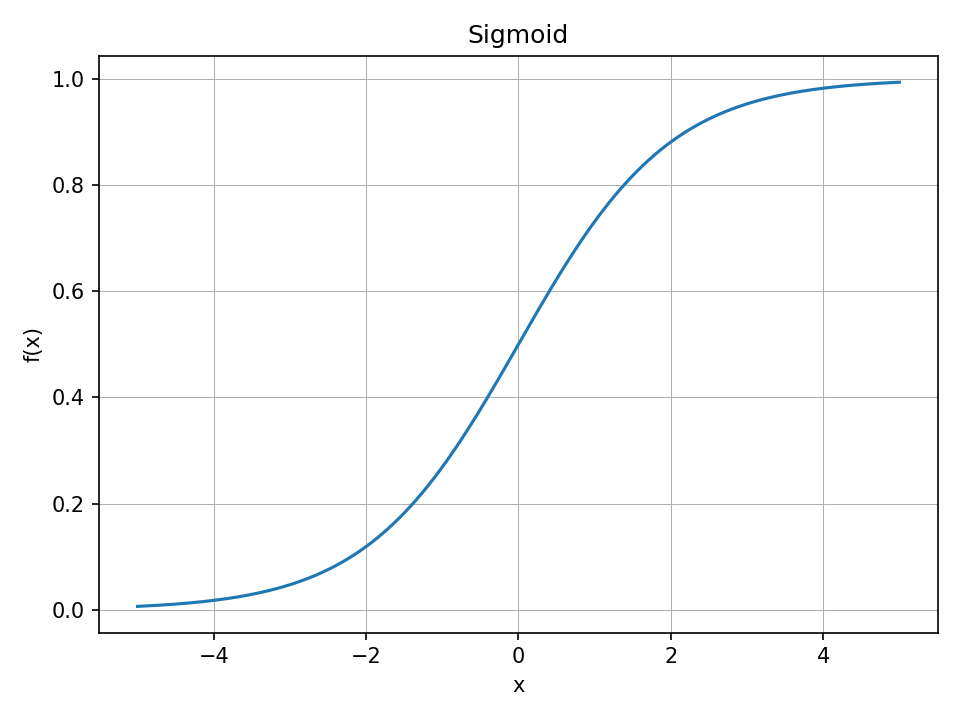
\includegraphics[width=4cm]{images/sigmoid.png}\\
\hline
\textbf{Tanh} (Tangens hyperbolicus) & $f(x) = \frac{e^x - e^{-x}}{e^x + e^{-x}}$ & $[-1, 1]$ & 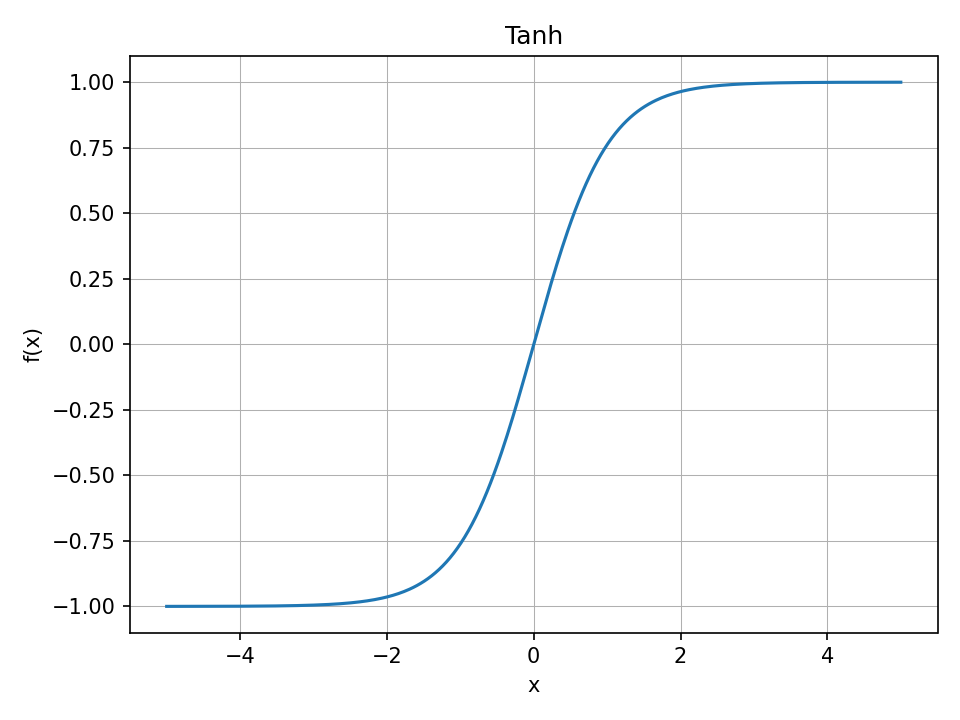
\includegraphics[width=4cm]{images/tanh.png}\\
\hline
\textbf{ReLU} (Rectified Linear Unit) & $f(x) = \max(0, x)$ & $[0, \infty]$ & 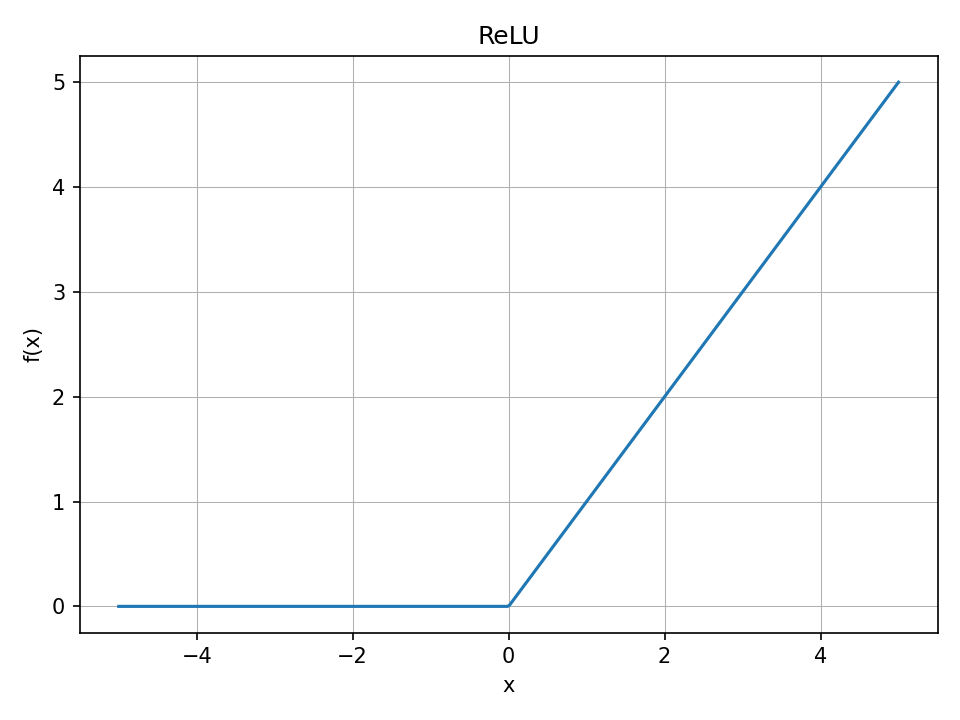
\includegraphics[width=4cm]{images/relu.png}\\
\hline
\textbf{SELU} (Scaled Exponential Linear Unit) & 
$f(x) = \lambda\begin{cases} 
x & \text{if } x > 0 \\
\alpha e^x - \alpha & \text{if } x \leq 0 
\end{cases}$ & $[-2, \infty]$ & 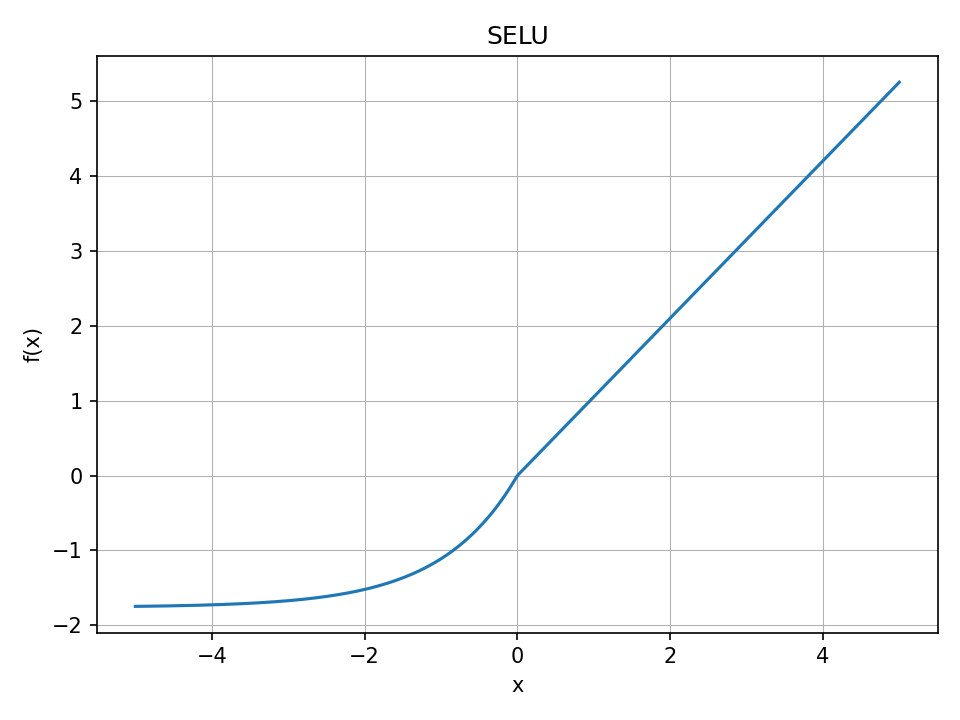
\includegraphics[width=4cm]{images/selu.png}\\
\hline
\end{tabular}
\caption{Activation Functions. Adapted from \cite{Berahmand24}}
\label{tab:activations_functions}
\end{table}

\paragraph{Number of Layers:} The number of layers in an autoencoder plays a critical role in determining its capacity to learn meaningful representations of input data. The depth of the network, defined by the number of layers, affects both the expressiveness and the generalization ability of the model. Shallow autoencoders, with only one or two hidden layers, may suffice for simple or low-dimensional data, offering computational efficiency and reduced risk of overfitting \cite{Berahmand24}. In contrast, deep autoencoders, which comprise multiple hidden layers in both the encoder and decoder, are better suited for capturing complex, hierarchical features, especially in high-dimensional datasets. However, increasing the number of layers also introduces challenges, including vanishing gradients, longer training times, and a higher demand for regularization techniques \cite{Charte18}. Because the optimal number of layers depends on the data characteristics and task complexity, we will first identify a suitable network depth through preliminary experiments before proceeding with further evaluations \cite{Goodfellow16}.

\paragraph{Number of Neurons per Layer:} The number of neurons in each layer is typically dictated by the dimensionality of the data. The input layer contains a number of neurons equal to the number of features in the input data, ensuring that each input dimension is represented. The output layer mirrors the input layer in size, especially in basic autoencoders, since the goal is to reconstruct the input from a compressed representation. Hidden layers, particularly the bottleneck or latent space layer, contain fewer neurons than the input or output layers to enforce dimensionality reduction. Additional hidden layers may exist in deeper autoencoders, often arranged symmetrically around the bottleneck to form the encoder and decoder components. The specific number of neurons in these hidden layers typically decreases toward the bottleneck and then increases symmetrically in the decoder \cite{Charte18}.

\paragraph{Size of Latent Space:} The size of the latent space in autoencoders plays a critical role in determining the model’s capacity to compress and reconstruct data effectively. A smaller latent space forces the model to learn more compact and informative representations by distilling the most salient features of the input data, which can enhance generalization and denoising performance but may also lead to underfitting if important information is lost. Conversely, a larger latent space allows for more detailed encoding of the input, potentially improving reconstruction fidelity but increasing the risk of overfitting, where the model memorizes rather than generalizes. The optimal size of the latent space is highly dependent on the complexity and intrinsic dimensionality of the data \cite{Berahmand24}. For the purposes of our experiments, we will use latent space sizes of 2 and 3, which, while relatively small, are particularly advantageous for visualization, allowing the encoded representations to be easily interpreted and plotted in two- or three-dimensional space.

\subsection{Loss Configurations}

Loss functions form the mathematical foundation for training neural networks by providing a quantitative measure of the model’s performance on a given task. In the context of autoencoders loss functions guide the optimization of two key components: the encoder and the decoder. The \emph{encoder}, denoted by a parametric function \( f_\theta: \mathbb{R}^n \rightarrow \mathbb{R}^m \), maps an input \( x \in \mathbb{R}^n \) to a lower-dimensional latent representation \( h = f_\theta(x) \). The \emph{decoder}, represented by \( g_\phi: \mathbb{R}^m \rightarrow \mathbb{R}^n \), attempts to reconstruct the original input from the latent code, yielding a reconstruction \( \hat{x} = g_\phi(h) = g_\phi(f_\theta(x)) \). The loss function \( \mathcal{L}: \mathbb{R}^n \times \mathbb{R}^n \rightarrow \mathbb{R}_{\geq 0} \) measures the discrepancy between the original input \( x \) and its reconstruction \( \hat{x} \), with the objective of minimizing this difference across the dataset. Formally, the training process seeks the parameters \( \theta \) and \( \phi \) that minimizes the loss. Different loss functions impose different assumptions on the data distribution and can be chosen to emphasize specific characteristics of the reconstruction. In the sections that follow, various loss functions will be introduced in terms of their mathematical formulation and practical relevance to training effective autoencoder models.

\paragraph{Mean Squared Error:} The Mean Squared Error (MSE) is a widely used loss function in autoencoders [\cite{Berahmand24}, \cite{Charte18}]. It evaluates the average of the squared differences between each input feature and its corresponding reconstruction. This squared formulation ensures that larger errors are penalized more heavily than smaller ones, encouraging the model to prioritize accurate reconstructions across all dimensions. Mathematically the MSE is defined as
\[
\mathcal{L}_{MSE}(x, \hat{x}) = \|x - \hat{x}\|^2_2 = \frac{1}{n}\sum_{i=1}^{n} (x_i - \hat{x}_i)^2 \ \cite{torch.nn}.
\]

\paragraph{Cosine Similarity:} Cosine similarity is a metric not frequently employed in the context of autoencoders. It measures the angular distance between two vectors in a high-dimensional space, offering a geometry-based assessment of similarity that is invariant to vector magnitude. In applications involving information retrieval tasks, cosine similarity serves as a valuable tool for comparing embeddings \cite{Xia15}. By focusing on the orientation rather than the length of the vectors, it effectively captures semantic closeness, which is especially useful when dealing with normalized feature representations. This becomes crucial in scenarios where the magnitude of embeddings may vary due to the nature of the data, but the directional alignment is preserved. Consequently, using cosine similarity in these scenarios allows autoencoders to be more robust in identifying relationships between inputs, enhancing the performance of tasks where understanding the relative positioning of data in feature space is more informative than absolute distances \cite{Zhang23}. Mathematically the cosine similarity is defined as
\[
\mathcal{L}_{CosSim}(x, \hat{x}) = \frac{x \cdot \hat{x}}{\|x\| \, \|\hat{x}\|} = \frac{\sum_{i=1}^{n} x_i \hat{x}_i}{\sqrt{\sum_{i=1}^{n} x_i^2} \cdot \sqrt{\sum_{i=1}^{n} \hat{x}_i^2}} \ \cite{torch.nn}.
\]

\paragraph{Kullback-Leibler Divergence:} The Kullback-Leibler Divergence (KL divergence) is a fundamental concept in information theory and plays a crucial role in neural networks, particularly in probabilistic models. It quantifies the discrepancy between two probability distributions and is often interpreted as the amount of information lost when an approximate distribution is used to represent a true distribution \cite{Kingma19}. In neural networks, KL divergence commonly appears in training objectives such as those for Variational Autoencoders (VAEs), where it acts as a regularization term that encourages the learned posterior to remain close to a prior distribution. In our case, however, we do not use the latent distributions of the KL divergence (as is standard in VAEs), but instead rely directly on the known probability densities of the samples. The form of the KL divergence, expressed as a loss function between the true distribution $p(x)$ and an approximate distribution $q(\hat{x})$, is given by:
\[
\mathcal{L}_{\text{KLD}}(x, \hat{x}) = p(x) \log \left( \frac{p(x)}{q(\hat{x})} \right) \ \cite{torch.nn}.
\]

\paragraph{Soft Trustworthiness:} The trustworthiness measure evaluates how accurately neighborhood relationships in a low-dimensional projection reflect the true proximities in the original high-dimensional data space. Specifically, it quantifies the degree to which the embedding introduces misleading neighbor relationships by including points that appear close in the projection but are actually distant in the original space. The trustworthiness score is calculated by identifying, for each data point, the projected neighbors that are not among its true nearest neighbors, and then summing the rank distances of these intruding points in the original space \cite{Venna01}. A lower cumulative error indicates a more trustworthy projection. This measure is scaled to fall between 0 and 1, where values closer to 1 signify higher trustworthiness. However, the original formulation of trustworthiness relies on discrete rank comparisons and set comparisons, which makes it non-differentiable and therefore unsuitable as a loss function in gradient-based optimization frameworks. To address this limitation, we developed a differentiable variant of the trustworthiness measure, enabling its integration into learning algorithms that optimize projection quality through gradient descent. Formally, for a neighborhood size $k$, the trustworthiness score is:
$$
T(k) \;=\; 1 \;-\;
\frac{2}{n\,k\,(2n-3k-1)}
\;\sum_{i=1}^{n}
\;\sum_{j \,\in\,N_i^k}
\bigl(r_X(i,j)\;-\;k\bigr) \ \cite{Venna01},
$$
where $N_i^k$ contains the "intrusions": points that appear among the $k$ nearest neighbors of sample $i$ in the embedding space $Z$ but not in the original space $X$, and $r_X(i,j)$ is the rank of point $j$ with respect to $i$ in the original space. This formulation ensures that $0 \le T(k) \le 1$, with higher values indicating greater fidelity of neighborhood preservation. 

To enable optimization via backpropagation, we present a novel, differentiable variant called the \textbf{Soft Trustworthiness}. In this formulation, discrete operations such as hard ranking and set membership are replaced by continuous approximations. The hard rank $r_X(i,j)$ is substituted with a \textbf{soft rank} $\widetilde r_X(i,j)$ computed via sigmoids:
$$
\widetilde r_X(i,j)
= 1 \;+\!
\sum_{\ell=1}^{n}
\sigma\!\left(\frac{D_X(i,j)\;-\;D_X(i,\ell)}{\tau_r}\right),
$$
$$
\text{where}
\quad
\sigma(x)=\frac{1}{1+e^{-x}}
,
\quad
D_X(i,j) = \|x_i - x_j\|_2
.
$$
A \textbf{soft top-$k$} membership weight $W_Z(i,j)$ is then defined using the same mechanism in the embedding space:
$$
W_Z(i,j) = \text{clamp}\left(\frac{k+1 - \widetilde r_Z(i,j)}{k},\, 0,\, 1\right)
$$
which smoothly approximates whether point $j$ belongs to the top-$k$ neighbors of $i$ in the embedding.
The final trustworthiness loss penalizes soft intrusions using a ReLU thresholded rank error:
$$
S_{i,j} \;=\;\bigl[k-\widetilde r_Y(i,j)\bigr]_{+},
\quad
[x]_{+}=\max(x,0),
$$
and aggregates the penalties across the batch:
$$
\mathcal L_{\rm softTW}(x, \hat{x})_k
= \frac{2}{n\,k\,(2n-3k-1)}\,
\sum_{i=1}^{n}\;\sum_{j=1}^{n}
\;S_{i,j}\;\bigl(1 - W_Z(i,j)\bigr).
$$
This differentiable formulation retains the conceptual structure of the original trustworthiness score but enables its use in learning objectives. As the temperature parameters $\tau_r$ and $\tau_s$ approach zero, the soft approximation converges to the original discrete version. With this contribution, we not only formalize a previously unpublished extension of the classic trustworthiness metric but also make it accessible for modern, gradient-based optimization techniques in representation learning.

\subsection{Supervised Extentions}

Supervised extensions enhance autoencoders by incorporating label information into training, guiding the model to learn embeddings that are both reconstructive and semantically meaningful. This is especially important for detecting in-between instances (IBIs), which exist between distinct clusters and are often overlooked by unsupervised methods. By introducing loss functions like triplet margin loss and cosine embedding loss, the model is encouraged to bring similar instances closer together and push dissimilar ones apart in the latent space. These supervised objectives promote better class separation and alignment, making the embeddings more suitable for tasks requiring fine-grained discrimination, such as IBI detection.

\paragraph{Triplet Margin Loss:} Triplet margin loss is a foundational component in deep metric learning, aiming to structure the embedding space such that samples from the same class are drawn closer together while those from different classes are pushed apart by at least a fixed margin \cite{Yang19}. For a given triplet consisting of an anchor $h_a$, a positive example $h_p$ from the same class, and a negative example $h_n$ from a different class, the loss function encourages the squared distance between the anchor and the positive to be smaller than the squared distance between the anchor and the negative by a margin $m > 0$. This is mathematically formulated as
$$
\mathcal{L}_{\text{TriMarg}}(h) = \max\{0, \, \|h_a - h_p\|_2 - \|h_a - h_n\|_2 + m \} \ \cite{torch.nn}.
$$
The incorporation of this loss steers the embedding space toward enhanced intra-class compactness and inter-class separability, which is particularly beneficial for distinguishing in-between instances.

\paragraph{Cosine Embedding Loss:} Cosine embedding loss is a metric learning objective commonly employed in tasks where understanding the similarity or dissimilarity between paired data points is crucial \cite{Singh18}. It evaluates how closely the angular relationship between two feature representations aligns with a target label. Given two vectors $h_i$ and $h_j$, and a label $y \in \{1, -1\}$ indicating whether the pair is similar or dissimilar, the cosine embedding loss is expressed as
$$
\mathcal{L}_{\text{CosEmb}}(h) = 
\begin{cases}
1 - \cos(h_i, h_j), & \text{if } y = 1 \\
\max\{0, \cos(h_i, h_j) - m\}, & \text{if } y = -1
\end{cases}
\ \cite{torch.nn},
$$
where $\cos(h_i, h_j) = \dfrac{h_i \cdot h_j}{\|h_i\| \|h_j\|}$ denotes the cosine similarity between the two vectors, and $m \in [0,1]$ is a margin that defines the maximum allowable similarity for dissimilar pairs. This loss encourages the model to generate embeddings that are directionally aligned when the inputs are semantically similar and angularly separated beyond the margin when they are not. Unlike the triplet margin loss, which requires triplet sampling, the cosine embedding loss functions on pairs, simplifying the sampling strategy while still enforcing semantic alignment.

\section{Evaluation Protocol}

The evaluation strategy adopted in this thesis relies on two principal methods: the quantitative analysis of loss values and the qualitative visual examination of the latent space. While both approaches contribute to understanding the performance of the autoencoder models, the visual analysis is considered the more informative and decisive component, particularly in the context of in-between instance (IBI) preservation.

Quantitative evaluation is carried out by monitoring loss values during training, using the specific objective functions associated with each experiment. While these metrics quantify the reconstruction fidelity or embedding structure in a mathematically rigorous way, their absolute values are not directly comparable across different loss functions due to differing scales and underlying assumptions. Moreover, a lower loss value does not necessarily imply improved IBI preservation, as the objectives may prioritize reconstruction accuracy or local neighborhood preservation without explicitly considering inter-cluster instances.

Given these limitations, greater emphasis is placed on visual examination of the latent representations produced by the autoencoders. Since all experiments constrain the latent space to two or three dimensions, the resulting embeddings can be plotted directly and interpreted visually. These visualizations provide critical insight into the geometric structure of the encoded data, such as the separation of clusters, the continuity of transitions between them, and the presence of points situated between distinct groupings. Patterns that are difficult to capture through scalar loss values, such as overlapping cluster boundaries or emerging bridges between classes, are often readily apparent through visual inspection.

Therefore, while loss values serve as a basic sanity check for training convergence and model stability, it is the qualitative structure of the latent space, revealed through visual analysis, that ultimately guides the interpretation of IBI preservation and model effectiveness in this study.

\section{Tools and System Specifications}

The computational experiments conducted in this thesis were performed on a high-performance desktop system running Windows 11 Pro 64-bit. The system was equipped with an AMD Ryzen 7 3700X processor, featuring eight cores operating at a base clock speed of 3.6 GHz. This multi-core architecture provided the parallel processing capabilities necessary to efficiently handle the training of deep neural networks, especially in the context of the iterative optimization routines required for autoencoder models. The system was also outfitted with 32 GB of DDR4 RAM clocked at 3.2 GHz, which ensured that the datasets and neural network parameters could be stored in memory without incurring performance bottlenecks. Although the machine included an NVIDIA GeForce GTX 1660 SUPER graphics card, no GPU acceleration was utilized during the training or evaluation of the models.

The entire software environment was implemented using Python 3.12.9 \cite{Python}, a language widely adopted in scientific computing and machine learning for its robust ecosystem and extensive library support. Core computational and visualization tasks were facilitated by several key libraries. NumPy 2.1.3 \cite{NumPy} was employed for numerical operations, particularly for managing multi-dimensional arrays and performing vectorized computations central to data preprocessing and loss function calculations. Matplotlib 3.10.0 \cite{Matplotlib} served as the primary tool for plotting, enabling visual inspection of reconstruction fidelity and latent space structures. Most crucially, PyTorch 2.5.1 \cite{PyTorch} was used as the deep learning framework for building, training, and evaluating the autoencoder architectures. PyTorch offers seamless integration with NumPy, making it particularly suitable for research scenarios that require experimentation with novel loss functions.
\newpage
\chapter{Experiments} \label{ch:experiments}

Building upon the methodological foundations outlined in the previous chapter, this section presents the empirical investigation designed to address the research questions of this work. The following sections detail the progression of these investigations, beginning with architectural variations, continuing with unsupervised loss objectives, and concluding with the contribution of supervised strategies to the preservation of transitional structure.

\section{Impact of Autoencoder Architecture on In-Between Instance Preservation} \label{sec:rq1}

\begin{table}[htb]
\centering
\renewcommand\cellalign{cc}
\renewcommand\theadalign{cc}

% ----- First Table -----
\begin{subtable}[t]{\textwidth}
\centering
\begin{tabular}{|
  >{\centering\arraybackslash}m{0.15cm} |
  >{\centering\arraybackslash}m{0.50cm} |
  >{\centering\arraybackslash}m{2.00cm} |
  >{\centering\arraybackslash}m{2.33cm} |
  >{\centering\arraybackslash}m{2.66cm} |
  >{\centering\arraybackslash}m{3.00cm} |}
  \hline
  & & \multicolumn{4}{c|}{Network Depth} \\
  \hline
  & & \textbf{0} & \textbf{1} & \textbf{2} & \textbf{3} \\
  \hline
  \multirow{7}{*}{\rotatebox[origin=c]{90}{\parbox[c][0.15cm][c]{4.5cm}{\centering Network Width}}} 
    & \boldmath{$2^0$} 
    & \makecell{\textcolor{red!60!black}{0.1449} \\ \textit{2-1}} 
    & \makecell{\textcolor{red!100!black}{0.1458} \\ \textit{2-1-1}} 
    & \makecell{\textcolor{red!80!black}{0.1453} \\ \textit{2-2-1-1}} 
    & \makecell{0.0063 \\ \textit{2-4-2-1-1}} \\
  \cline{2-6}
  & \boldmath{$2^1$} 
    &  
    & \makecell{\textcolor{red!40!black}{0.0641} \\ \textit{2-2-1}} 
    & \makecell{\textcolor{red!20!black}{0.0374} \\ \textit{2-4-2-1}} 
    & \makecell{\textcolor{green!60!black}{0.0019} \\ \textit{2-8-4-2-1}} \\
  \cline{2-6}
  & \boldmath{$2^2$} 
    &  
    & \makecell{0.0171 \\ \textit{2-4-1}} 
    & \makecell{0.0094 \\ \textit{2-8-4-1}} 
    & \makecell{\textcolor{green!40!black}{0.0020} \\ \textit{2-16-8-4-1}} \\
  \cline{2-6}
  & \boldmath{$2^3$} 
    &  
    & \makecell{0.0049 \\ \textit{2-8-1}} 
    & \makecell{\textcolor{green!80!black}{0.0017} \\ \textit{2-16-8-1}} 
    & \makecell{\textcolor{green!100!black}{0.0016} \\ \textit{2-32-16-8-1}} \\
  \cline{2-6}
  & \boldmath{$2^4$} 
    &  
    & \makecell{0.0036 \\ \textit{2-16-1}} 
    & \makecell{\textcolor{green!60!black}{0.0019} \\ \textit{2-32-16-1}} 
    & \makecell{\textcolor{green!40!black}{0.0020} \\ \textit{2-64-32-16-1}} \\
  \cline{2-6}
  & \boldmath{$2^5$} 
    &  
    & \makecell{\textcolor{green!20!black}{0.0026} \\ \textit{2-32-1}} 
    & \makecell{\textcolor{green!60!black}{0.0019} \\ \textit{2-64-32-1}} 
    & \makecell{\textcolor{green!20!black}{0.0026} \\ \textit{2-128-64-32-1}} \\
  \hline
\end{tabular}
\caption{2D autoencoder.}
\label{tab:rq1-2d}
\end{subtable}

\vspace{1em} % spacing between tables

% ----- Second Table -----
\begin{subtable}[t]{\textwidth}
\centering
\begin{tabular}{|
  >{\centering\arraybackslash}m{0.15cm} |
  >{\centering\arraybackslash}m{0.50cm} |
  >{\centering\arraybackslash}m{2.00cm} |
  >{\centering\arraybackslash}m{2.33cm} |
  >{\centering\arraybackslash}m{2.66cm} |
  >{\centering\arraybackslash}m{3.00cm} |}
  \hline
  & & \multicolumn{4}{c|}{Network Depth} \\
  \hline
  & & \textbf{0} & \textbf{1} & \textbf{2} & \textbf{3} \\
  \hline
  \multirow{7}{*}{\rotatebox[origin=c]{90}{\parbox[c][0.15cm][c]{5.5cm}{\centering Network Width}}} 
    & \boldmath{$2^0$} 
    & \makecell{\textcolor{red!40!black}{2.1619} \\ \textit{3-2}} 
    & \makecell{\textcolor{red!100!black}{4.3859} \\ \textit{3-1-2}} 
    & \makecell{\textcolor{red!80!black}{3.4299} \\ \textit{3-2-1-2}} 
    & \makecell{\textcolor{red!20!black}{2.1483} \\ \textit{3-4-2-1-2}} \\
  \cline{2-6}
  & \boldmath{$2^1$} 
    &  
    & \makecell{\textcolor{red!60!black}{2.1625} \\ \textit{3-2-2}} 
    & \makecell{0.6318 \\ \textit{3-4-2-2}} 
    & \makecell{0.2784 \\ \textit{3-8-4-2-2}} \\
  \cline{2-6}
  & \boldmath{$2^2$} 
    &  
    & \makecell{0.5070 \\ \textit{3-4-2}} 
    & \makecell{0.2157 \\ \textit{3-8-4-2}} 
    & \makecell{0.1488 \\ \textit{3-16-8-4-2}} \\
  \cline{2-6}
  & \boldmath{$2^3$} 
    &  
    & \makecell{0.3851 \\ \textit{3-8-2}} 
    & \makecell{0.1397 \\ \textit{3-16-8-2}} 
    & \makecell{\textcolor{green!40!black}{0.1116} \\ \textit{3-32-16-8-2}} \\
  \cline{2-6}
  & \boldmath{$2^4$} 
    &  
    & \makecell{0.2232 \\ \textit{3-16-2}} 
    & \makecell{\textcolor{green!60!black}{0.1018} \\ \textit{3-32-16-2}} 
    & \makecell{\textcolor{green!100!black}{0.0920} \\ \textit{3-64-32-16-2}} \\  
  \cline{2-6}
  & \boldmath{$2^5$} 
    &  
    & \makecell{0.1696 \\ \textit{3-32-2}} 
    & \makecell{\textcolor{green!80!black}{0.0936} \\ \textit{3-64-32-2}} 
    & \makecell{\textcolor{green!20!black}{0.1131} \\ \textit{3-128-64-32-2}} \\
  \hline
\end{tabular}
\caption{3D autoencoder.}
\label{tab:rq1-3d}
\end{subtable}

% ----- Main Caption -----
\caption{Grid search results across 2D and 3D autoencoders. Each cell displays the mean squared error (MSE) loss (top) and the corresponding encoder architecture (bottom). Network width indicates the number of units in the first layer both before and after the bottleneck, and network depth refers to the number of hidden layers in the encoder. The top and worst 5 results are visually highlighted.}
\label{tab:rq1-combined}
\end{table}

\begin{figure}[htb]
    \centering
    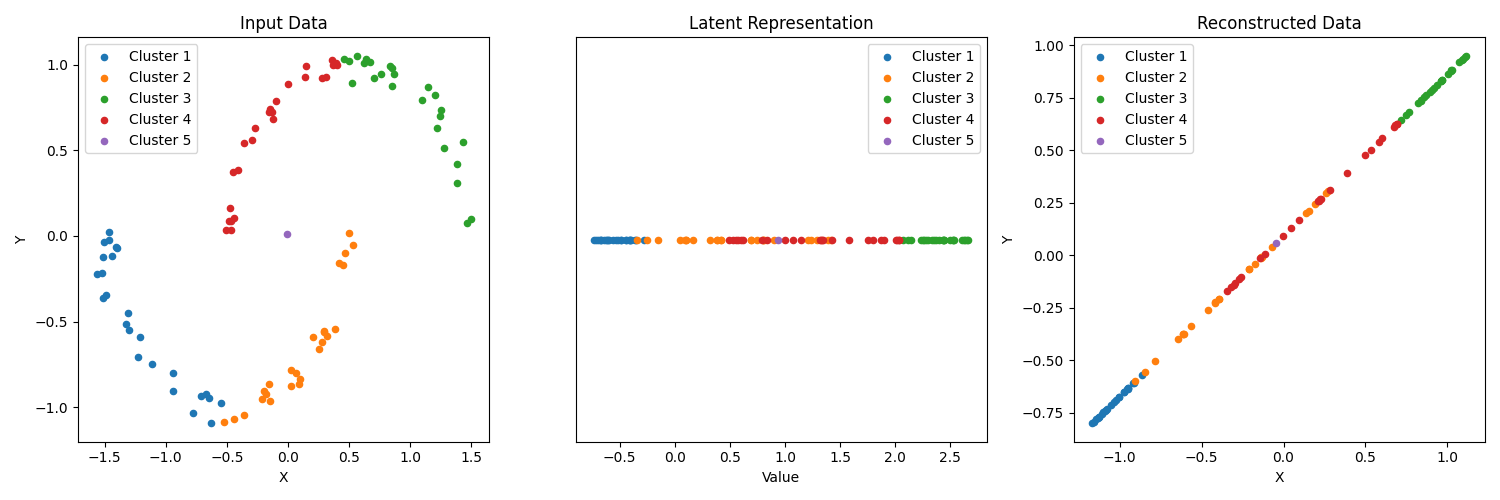
\includegraphics[width=\linewidth]{images/RQ1/2-1_0.1449.png}
    \caption{Baseline projections for a 2D autoencoder with no hidden layers (2–1 architecture) and \textcolor{red!60!black}{0.1449} MSE. This linear mapping serves as a reference.}
    \label{fig:2-1}
\end{figure}

\begin{figure}[htb]
  \centering
  % subfigure 1
  \begin{subfigure}[b]{0.49\textwidth}
    \centering
    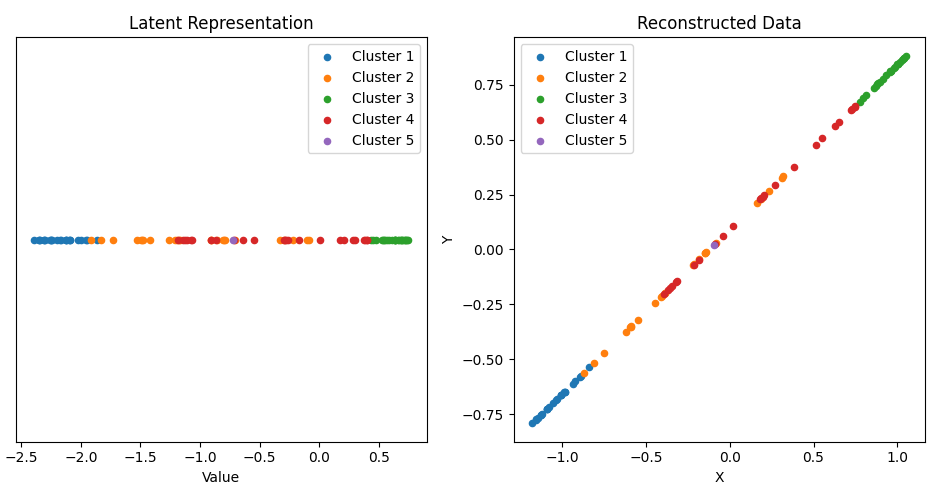
\includegraphics[width=\linewidth]{images/RQ1/2-1-1_0.1458.png}
    \caption{2-1-1 architecture with \textcolor{red!100!black}{0.1458} MSE.}
    \label{fig:2-1-1}
  \end{subfigure}
  \hfill
  % subfigure 2
  \begin{subfigure}[b]{0.49\textwidth}
    \centering
    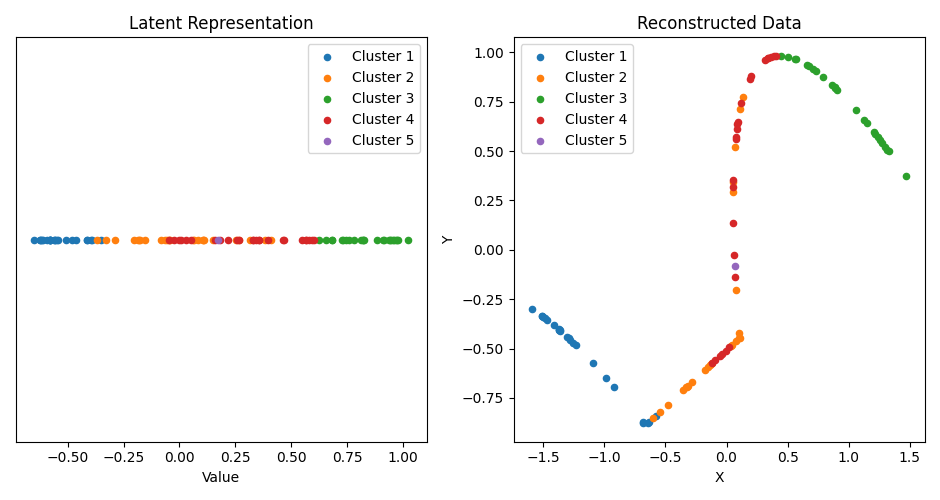
\includegraphics[width=\linewidth]{images/RQ1/2-2-1_0.0641.png}
    \caption{2-2-1 architecture with \textcolor{red!40!black}{0.0641} MSE.}
    \label{fig:2-2-1}
  \end{subfigure}
  \hfill
  % subfigure 3
  \begin{subfigure}[b]{0.49\textwidth}
    \centering
    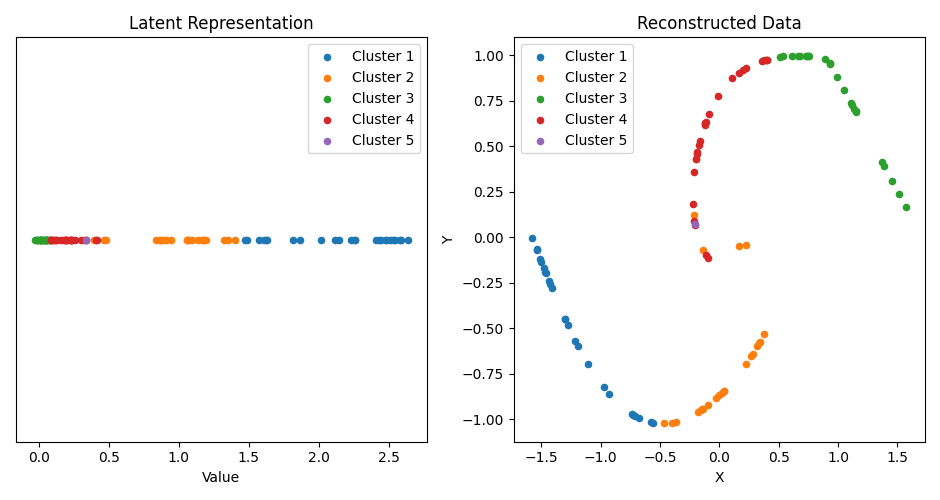
\includegraphics[width=\linewidth]{images/RQ1/2-4-1_0.0171.png}
    \caption{2-4-1 architecture with 0.0171 MSE.}
    \label{fig:2-4-1}
  \end{subfigure}
  \hfill
  % subfigure 4
  \begin{subfigure}[b]{0.49\textwidth}
    \centering
    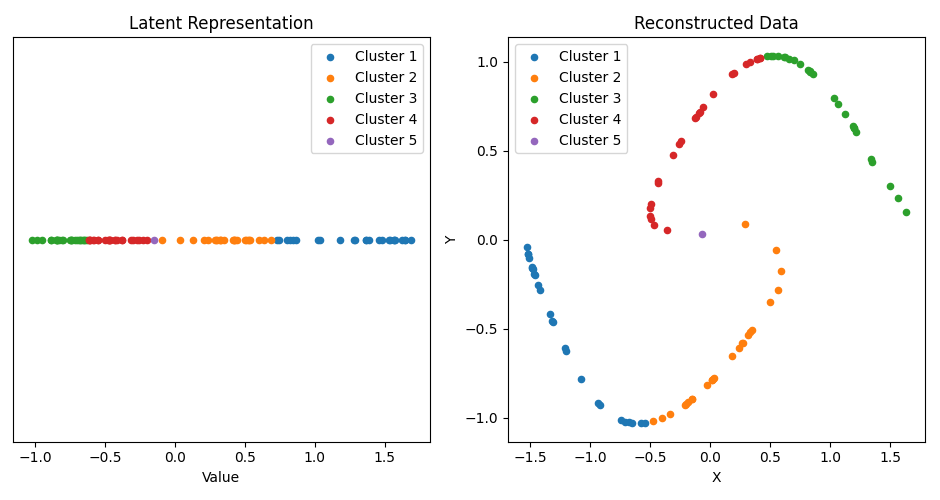
\includegraphics[width=\linewidth]{images/RQ1/2-8-1_0.0049.png}
    \caption{2-8-1 architecture with 0.0049 MSE.}
    \label{fig:2-8-1}
  \end{subfigure}
  \hfill
  % subfigure 5
  \begin{subfigure}[b]{0.49\textwidth}
    \centering
    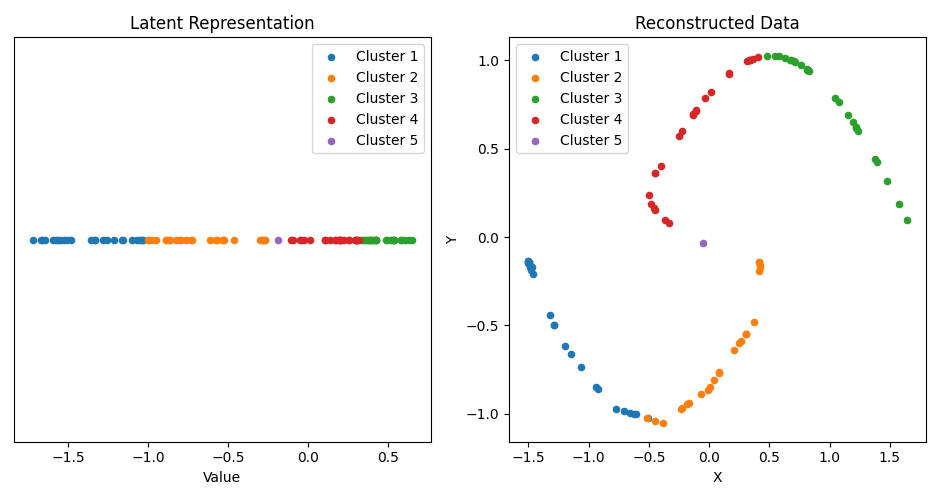
\includegraphics[width=\linewidth]{images/RQ1/2-16-1_0.0036.png}
    \caption{2-16-1 architecture with 0.0036 MSE.}
    \label{fig:2-16-1}
  \end{subfigure}
  \hfill
  % subfigure 6
  \begin{subfigure}[b]{0.49\textwidth}
    \centering
    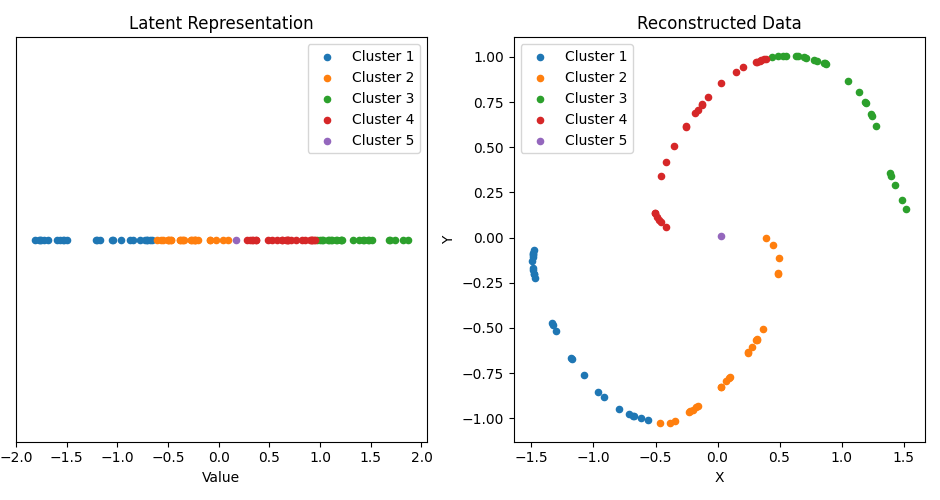
\includegraphics[width=\linewidth]{images/RQ1/2-32-1_0.0026.png}
    \caption{2-32-1 architecture with \textcolor{green!20!black}{0.0026} MSE.}
    \label{fig:2-32-1}
  \end{subfigure}

  \caption{Projections for 2D autoencoders with a single hidden layer of varying width. 2-X-1 architectures are compared.}
  \label{fig:2-X-1}
\end{figure}

\begin{figure}[htb]
  \centering
  % subfigure 1
  \begin{subfigure}[b]{0.49\textwidth}
    \centering
    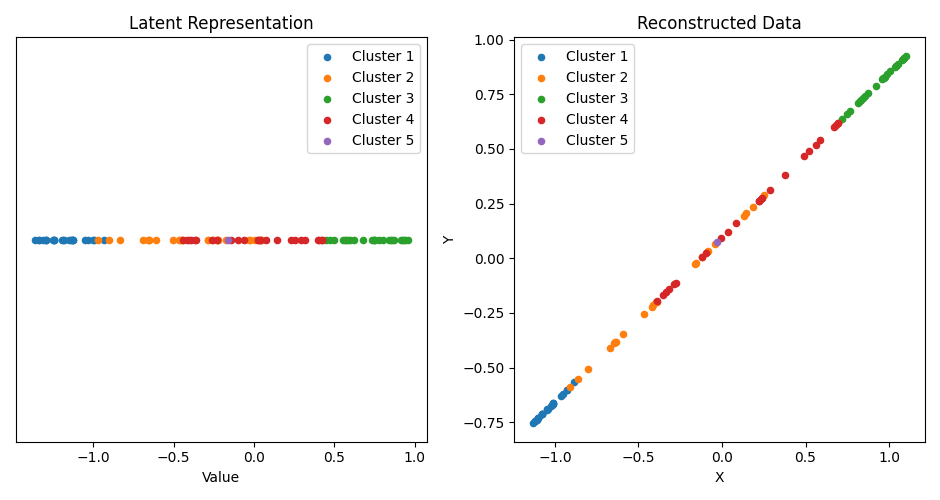
\includegraphics[width=\linewidth]{images/RQ1/2-2-1-1_0.1453.png}
    \caption{2-2-1-1 architecture with \textcolor{red!80!black}{0.1453} MSE.}
    \label{fig:2-2-1-1-2}
  \end{subfigure}
  \hfill
  % subfigure 2
  \begin{subfigure}[b]{0.49\textwidth}
    \centering
    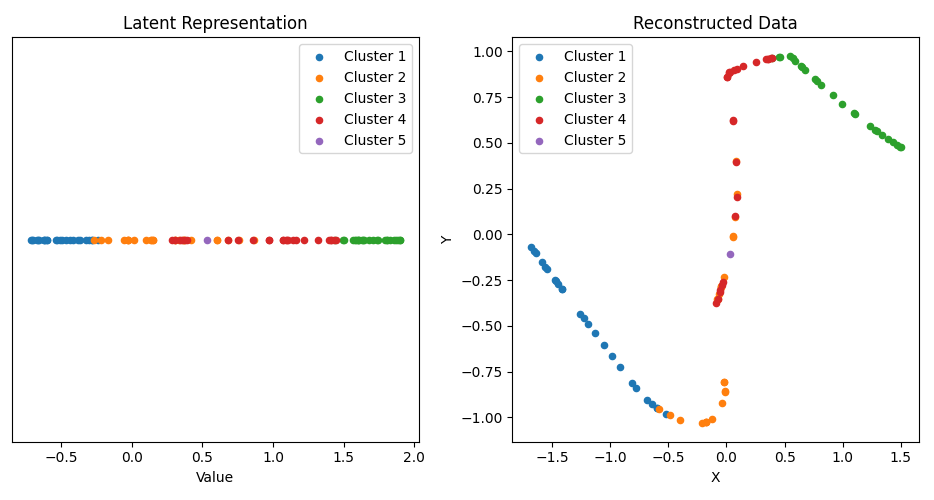
\includegraphics[width=\linewidth]{images/RQ1/2-4-2-1_0.0374.png}
    \caption{2-4-2-1 architecture with \textcolor{red!20!black}{0.0374} MSE.}
    \label{fig:2-4-2-1}
  \end{subfigure}
  \hfill
  % subfigure 3
  \begin{subfigure}[b]{0.49\textwidth}
    \centering
    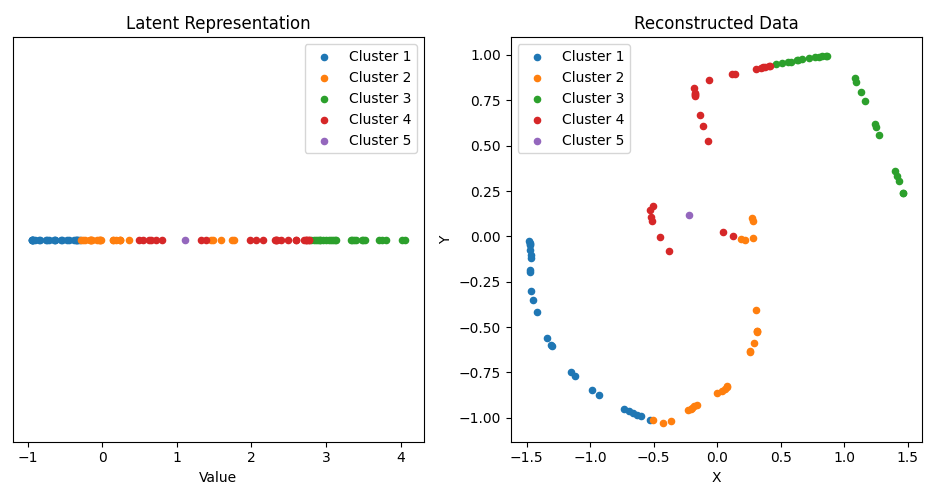
\includegraphics[width=\linewidth]{images/RQ1/2-8-4-1_0.0094.png}
    \caption{2-8-4-1 architecture with 0.0094 MSE.}
    \label{fig:2-8-4-1}
  \end{subfigure}
  \hfill
  % subfigure 4
  \begin{subfigure}[b]{0.49\textwidth}
    \centering
    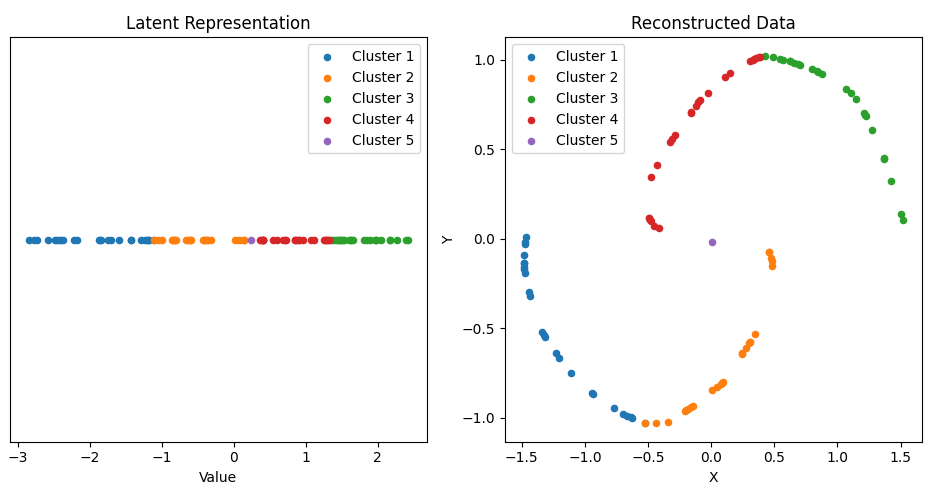
\includegraphics[width=\linewidth]{images/RQ1/2-16-8-1_0.0017.png}
    \caption{2-16-8-1 architecture with \textcolor{green!80!black}{0.0017} MSE.}
    \label{fig:2-16-8-1}
  \end{subfigure}
  \hfill
  % subfigure 5
  \begin{subfigure}[b]{0.49\textwidth}
    \centering
    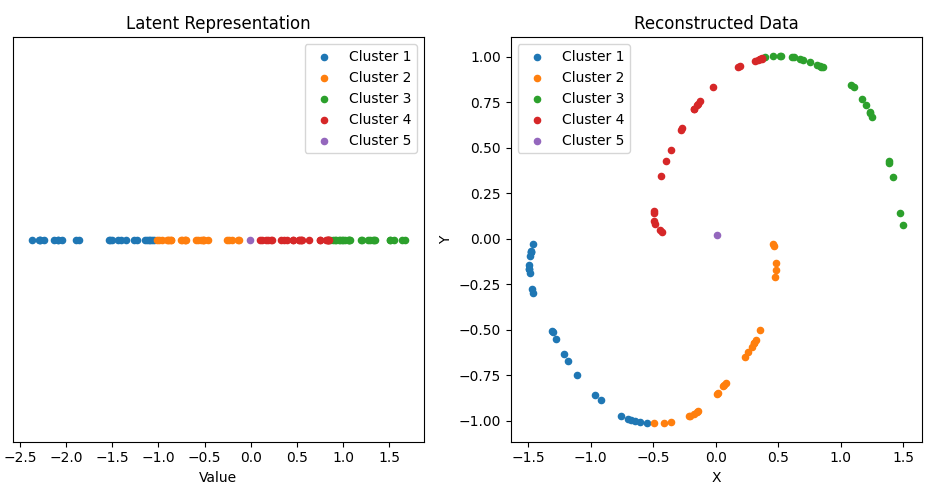
\includegraphics[width=\linewidth]{images/RQ1/2-32-16-1_0.0019.png}
    \caption{2-32-16-1 architecture with \textcolor{green!60!black}{0.0019} MSE.}
    \label{fig:2-32-16-1}
  \end{subfigure}
  \hfill
  % subfigure 6
  \begin{subfigure}[b]{0.49\textwidth}
    \centering
    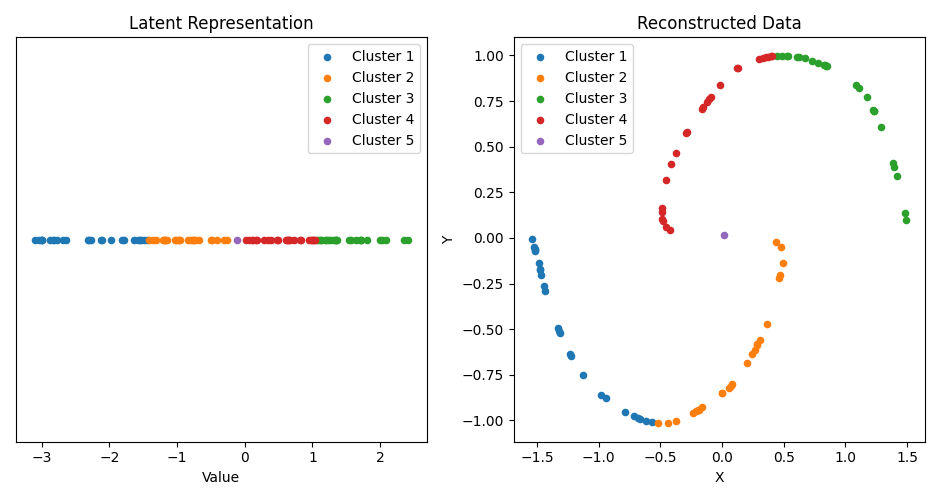
\includegraphics[width=\linewidth]{images/RQ1/2-64-32-1_0.0019.png}
    \caption{2-64-32-1 architecture with \textcolor{green!60!black}{0.0019} MSE.}
    \label{fig:2-64-32-1}
  \end{subfigure}

  \caption{Projections for 2D autoencoders with two hidden layers of varying width. 2-X-Y-1 architectures are compared.}
  \label{fig:2-X-Y-1}
\end{figure}

\begin{figure}[htb]
  \centering
  % subfigure 1
  \begin{subfigure}[b]{0.49\textwidth}
    \centering
    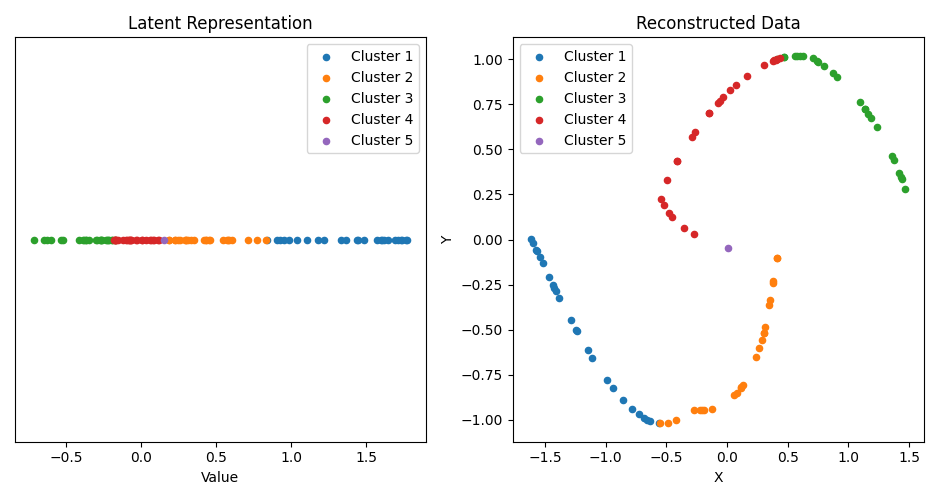
\includegraphics[width=\linewidth]{images/RQ1/2-4-2-1-1_0.0063.png}
    \caption{2-4-2-1-1 architecture with 0.0063 MSE.}
    \label{fig:2-4-2-1-1}
  \end{subfigure}
  \hfill
  % subfigure 2
  \begin{subfigure}[b]{0.49\textwidth}
    \centering
    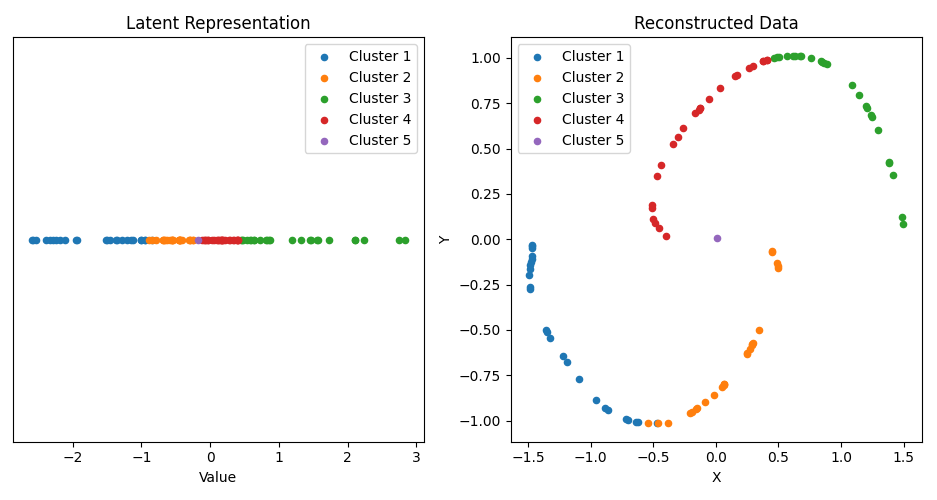
\includegraphics[width=\linewidth]{images/RQ1/2-8-4-2-1_0.0019.png}
    \caption{2-8-4-2-1 architecture with \textcolor{green!60!black}{0.0019} MSE.}
    \label{fig:2-8-4-2-1}
  \end{subfigure}
  \hfill
  % subfigure 3
  \begin{subfigure}[b]{0.49\textwidth}
    \centering
    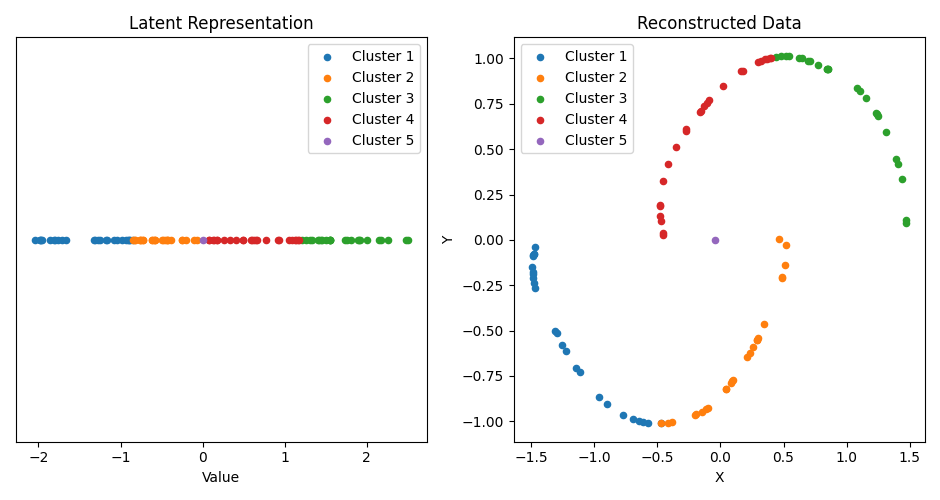
\includegraphics[width=\linewidth]{images/RQ1/2-16-8-4-1_0.0020.png}
    \caption{2-16-8-4-1 architecture with \textcolor{green!40!black}{0.0020} MSE.}
    \label{fig:2-16-8-4-1}
  \end{subfigure}
  \hfill
  % subfigure 4
  \begin{subfigure}[b]{0.49\textwidth}
    \centering
    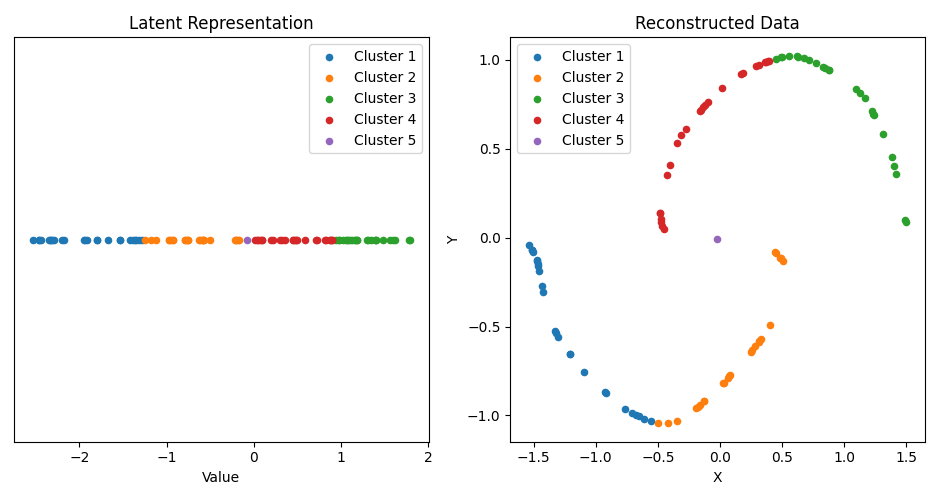
\includegraphics[width=\linewidth]{images/RQ1/2-32-16-8-1_0.0016.png}
    \caption{2-32-16-8-1 architecture with \textcolor{green!100!black}{0.0016} MSE.}
    \label{fig:2-32-16-8-1}
  \end{subfigure}
  \hfill
  % subfigure 5
  \begin{subfigure}[b]{0.49\textwidth}
    \centering
    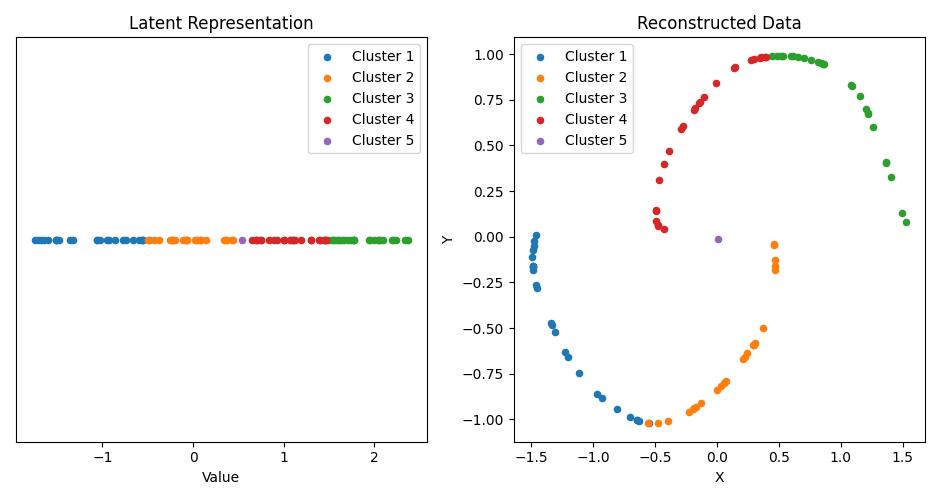
\includegraphics[width=\linewidth]{images/RQ1/2-64-32-16-1_0.0020.png}
    \caption{2-64-32-16-1 architecture with \textcolor{green!40!black}{0.0020} MSE.}
    \label{fig:2-64-32-16-1}
  \end{subfigure}
  \hfill
  % subfigure 6
  \begin{subfigure}[b]{0.49\textwidth}
    \centering
    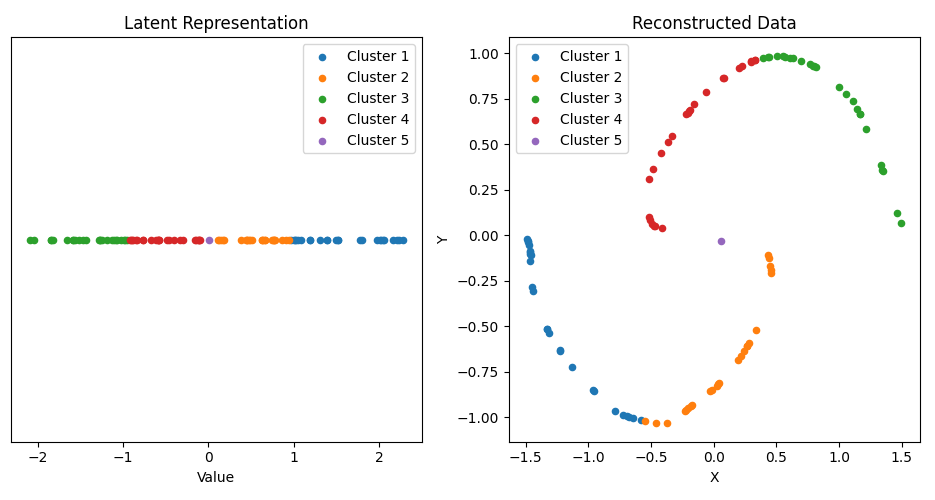
\includegraphics[width=\linewidth]{images/RQ1/2-128-64-32-1_0.0026.png}
    \caption{2-128-64-32-1 architecture with \textcolor{green!20!black}{0.0026} MSE.}
    \label{fig:2-128-64-32-1}
  \end{subfigure}

  \caption{Projections for 2D autoencoders with three hidden layers of varying width. 2-X-Y-Z-1 architectures are compared.}
  \label{fig:2-X-Y-Z-1}
\end{figure}

\begin{figure}[htb]
    \centering
    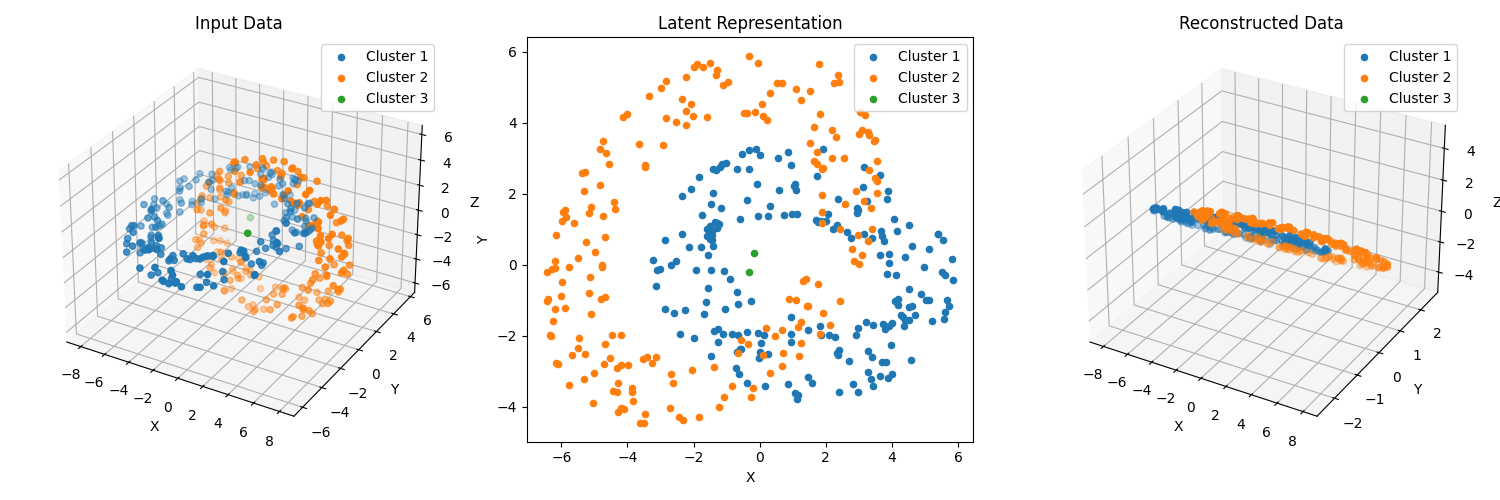
\includegraphics[width=\linewidth]{images/RQ1/3-2_2.1619.png}
    \caption{Baseline projections for a 3D autoencoder with no hidden layers (3–2 architecture) and \textcolor{red!40!black}{2.1619} MSE. This linear mapping serves as a reference.}
    \label{fig:3-2}
\end{figure}

\begin{figure}[htb]
  \centering
  % subfigure 1
  \begin{subfigure}[b]{0.49\textwidth}
    \centering
    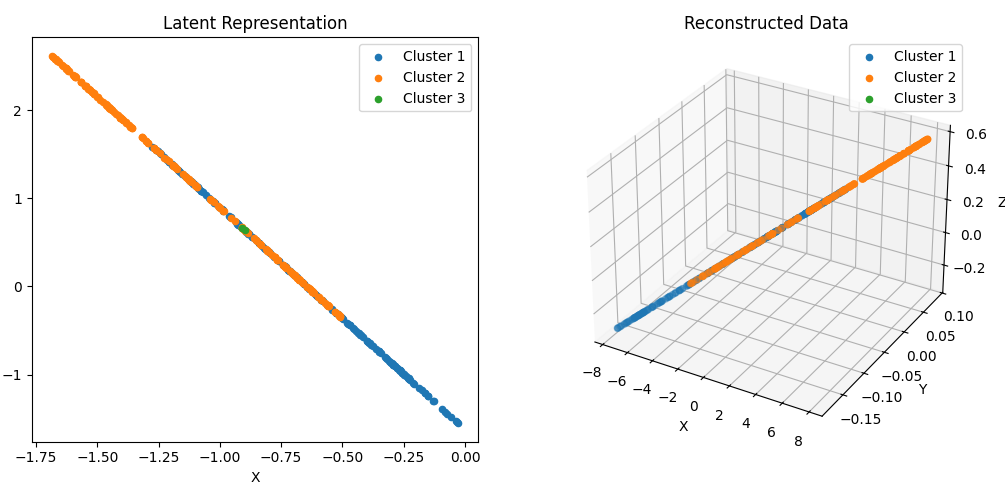
\includegraphics[width=\linewidth]{images/RQ1/3-1-2_4.3859.png}
    \caption{3-1-2 architecture with \textcolor{red!100!black}{4.3859} MSE.}
    \label{fig:3-1-2}
  \end{subfigure}
  \hfill
  % subfigure 2
  \begin{subfigure}[b]{0.49\textwidth}
    \centering
    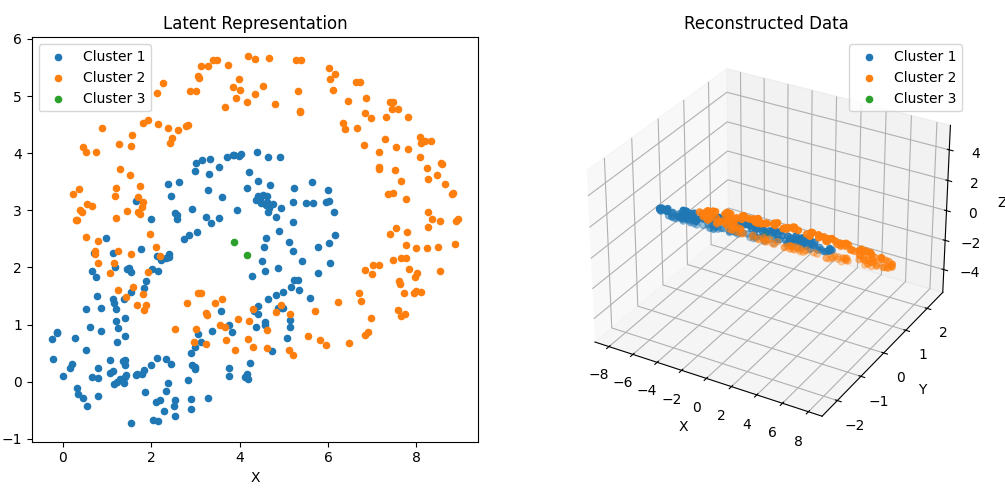
\includegraphics[width=\linewidth]{images/RQ1/3-2-2_2.1625.png}
    \caption{3-2-2 architecture with \textcolor{red!60!black}{2.1625} MSE.}
    \label{fig:3-2-2}
  \end{subfigure}
  \hfill
  % subfigure 3
  \begin{subfigure}[b]{0.49\textwidth}
    \centering
    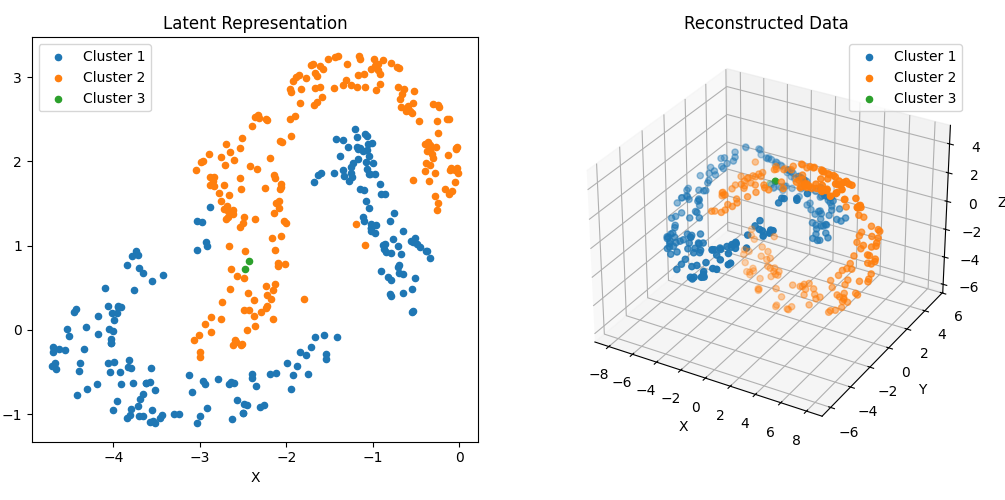
\includegraphics[width=\linewidth]{images/RQ1/3-4-2_0.5070.png}
    \caption{3-4-2 architecture with 0.5070 MSE.}
    \label{fig:3-4-2}
  \end{subfigure}
  \hfill
  % subfigure 4
  \begin{subfigure}[b]{0.49\textwidth}
    \centering
    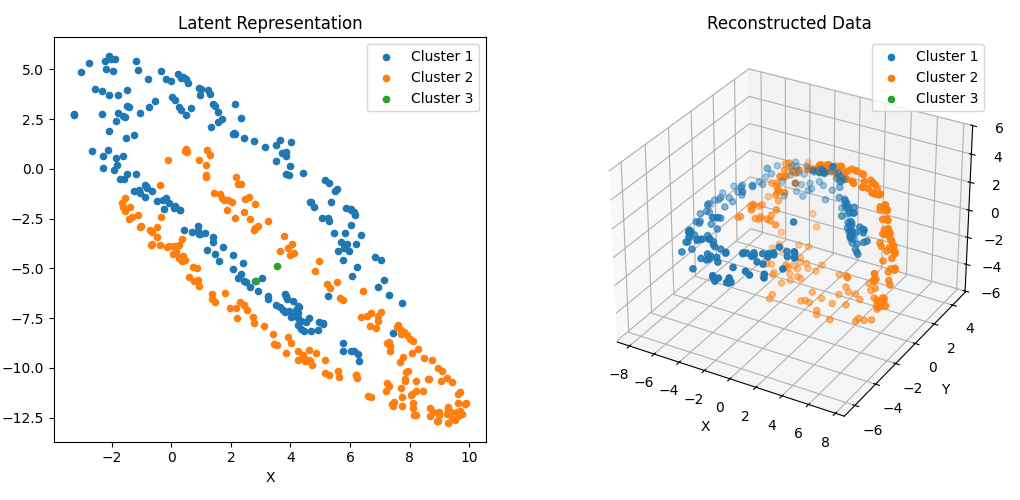
\includegraphics[width=\linewidth]{images/RQ1/3-8-2_0.3851.png}
    \caption{3-8-2 architecture with 0.3851 MSE.}
    \label{fig:3-8-2}
  \end{subfigure}
  \hfill  
  % subfigure 5
  \begin{subfigure}[b]{0.49\textwidth}
    \centering
    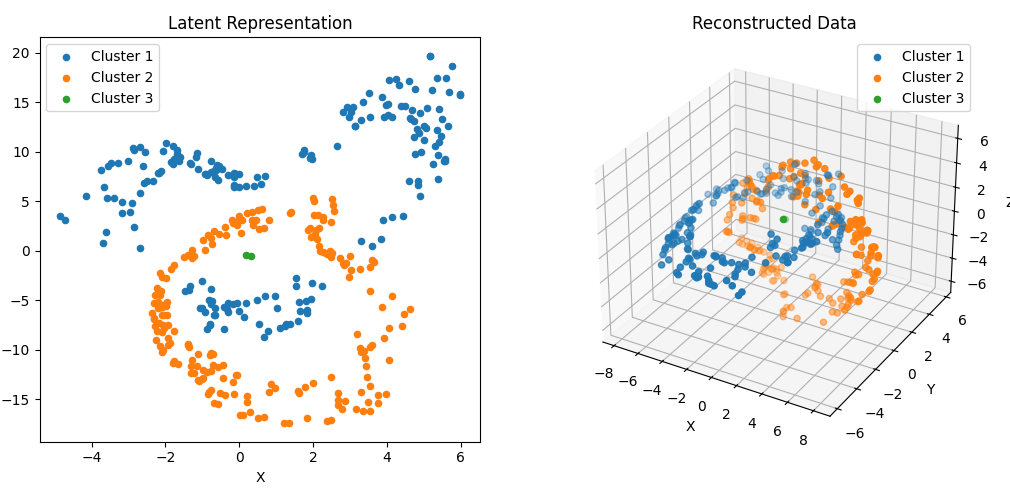
\includegraphics[width=\linewidth]{images/RQ1/3-16-2_0.2232.png}
    \caption{3-16-2 architecture with 0.2232 MSE.}
    \label{fig:3-16-2}
  \end{subfigure}
  \hfill  
  % subfigure 6
  \begin{subfigure}[b]{0.49\textwidth}
    \centering
    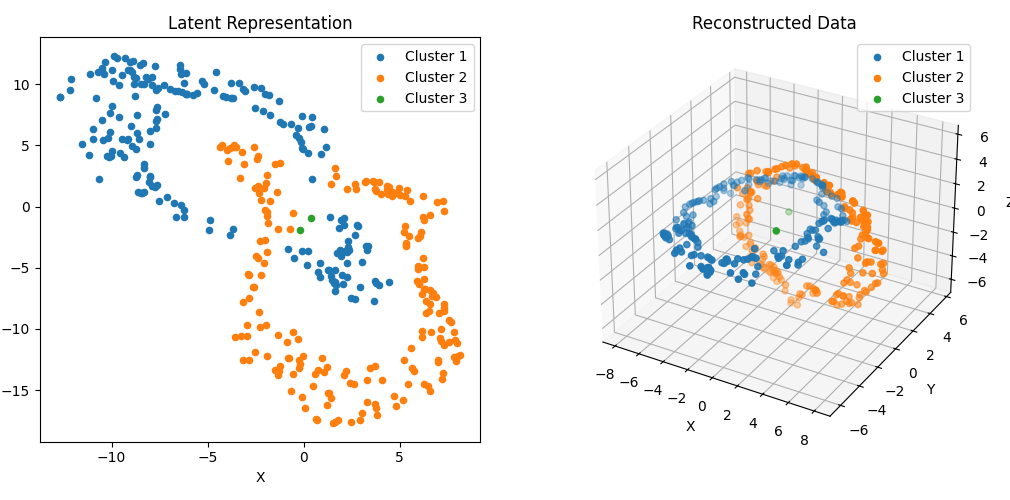
\includegraphics[width=\linewidth]{images/RQ1/3-32-2_0.1696.png}
    \caption{3-32-2 architecture with 0.1696 MSE.}
    \label{fig:3-32-2}
  \end{subfigure}

  \caption{Projections for 3D autoencoders with one hidden layer of varying width. 3-X-2 architectures are compared.}
  \label{fig:3-X-2}
\end{figure}

\begin{figure}[htb]
  \centering
  % subfigure 1
  \begin{subfigure}[b]{0.49\textwidth}
    \centering
    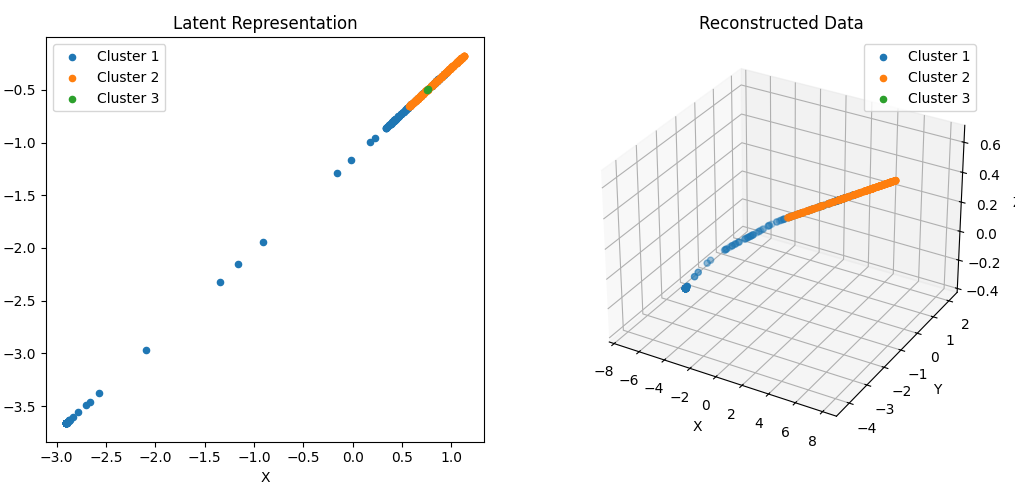
\includegraphics[width=\linewidth]{images/RQ1/3-2-1-2_3.4299.png}
    \caption{3-2-1-2 architecture with \textcolor{red!80!black}{3.4299} MSE.}
    \label{fig:3-2-1-2}
  \end{subfigure}
  \hfill
  % subfigure 2
  \begin{subfigure}[b]{0.49\textwidth}
    \centering
    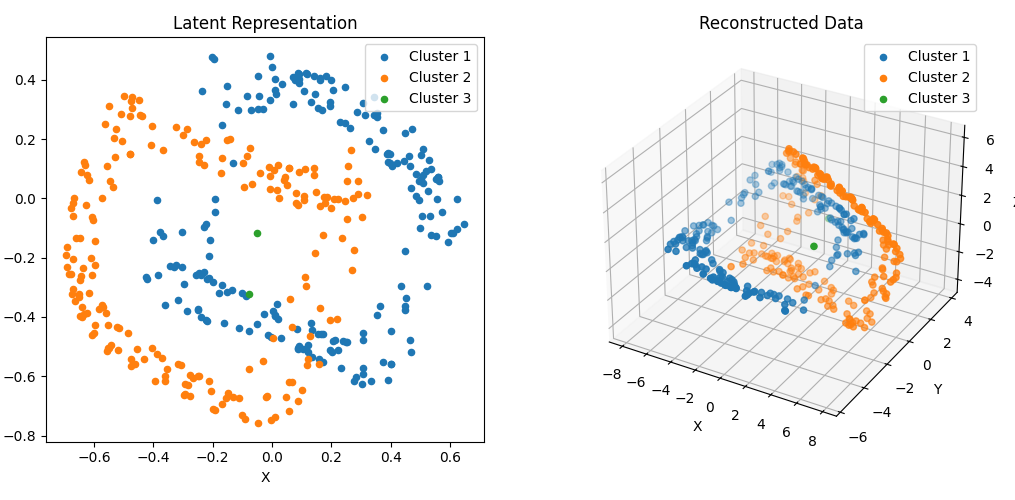
\includegraphics[width=\linewidth]{images/RQ1/3-4-2-2_0.6318.png}
    \caption{3-4-2-2 architecture with 0.6318 MSE.}
    \label{fig:3-4-2-2}
  \end{subfigure}
  \hfill
  % subfigure 3
  \begin{subfigure}[b]{0.49\textwidth}
    \centering
    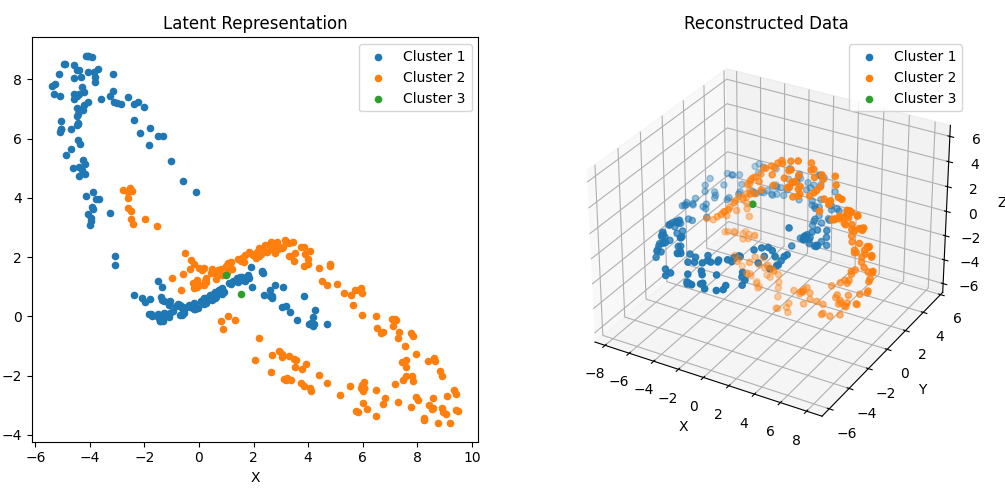
\includegraphics[width=\linewidth]{images/RQ1/3-8-4-2_0.2157.png}
    \caption{3-8-4-2 architecture with 0.2157 MSE.}
    \label{fig:3-8-4-2}
  \end{subfigure}
  \hfill
  % subfigure 4
  \begin{subfigure}[b]{0.49\textwidth}
    \centering
    \includegraphics[width=\linewidth]{images/RQ1/3-16-8-2_0.1397.png}
    \caption{3-16-8-2 architecture with 0.1397 MSE.}
    \label{fig:3-16-8-2}
  \end{subfigure}
  \hfill  
  % subfigure 5
  \begin{subfigure}[b]{0.49\textwidth}
    \centering
    \includegraphics[width=\linewidth]{images/RQ1/3-32-16-2_0.1018.png}
    \caption{3-32-16-2 architecture with \textcolor{green!60!black}{0.1018} MSE.}
    \label{fig:3-32-16-2}
  \end{subfigure}
  \hfill  
  % subfigure 6
  \begin{subfigure}[b]{0.49\textwidth}
    \centering
    \includegraphics[width=\linewidth]{images/RQ1/3-64-32-2_0.0936.png}
    \caption{3-64-32-2 architecture with \textcolor{green!80!black}{0.0936} MSE.}
    \label{fig:3-64-32-2}
  \end{subfigure}

  \caption{Projections for 3D autoencoders with two hidden layers of varying width. 3-X-Y-2 architectures are compared.}
  \label{fig:3-X-Y-2}
\end{figure}

\begin{figure}[htb]
  \centering
  % subfigure 1
  \begin{subfigure}[b]{0.49\textwidth}
    \centering
    \includegraphics[width=\linewidth]{images/RQ1/3-4-2-1-2_2.1483.png}
    \caption{3-4-2-1-2 architecture with \textcolor{red!20!black}{2.1483} MSE.}
    \label{fig:3-4-2-1-2}
  \end{subfigure}
  \hfill
  % subfigure 2
  \begin{subfigure}[b]{0.49\textwidth}
    \centering
    \includegraphics[width=\linewidth]{images/RQ1/3-8-4-2-2_0.2784.png}
    \caption{3-8-4-2-2 architecture with 0.2784 MSE.}
    \label{fig:3-8-4-2-2}
  \end{subfigure}
  \hfill
  % subfigure 3
  \begin{subfigure}[b]{0.49\textwidth}
    \centering
    \includegraphics[width=\linewidth]{images/RQ1/3-16-8-4-2_0.1488.png}
    \caption{3-16-8-4-2 architecture with 0.1488 MSE.}
    \label{fig:3-16-8-4-2}
  \end{subfigure}
  \hfill
  % subfigure 4
  \begin{subfigure}[b]{0.49\textwidth}
    \centering
    \includegraphics[width=\linewidth]{images/RQ1/3-32-16-8-2_0.1116.png}
    \caption{3-32-16-8-2 architecture with \textcolor{green!40!black}{0.1116} MSE.}
    \label{fig:3-32-16-8-2}
  \end{subfigure}
  \hfill  
  % subfigure 5
  \begin{subfigure}[b]{0.49\textwidth}
    \centering
    \includegraphics[width=\linewidth]{images/RQ1/3-64-32-16-2_0.0920.png}
    \caption{3-64-32-16-2 architecture with \textcolor{green!100!black}{0.0920} MSE.}
    \label{fig:3-64-32-16-2}
  \end{subfigure}
  \hfill  
  % subfigure 6
  \begin{subfigure}[b]{0.49\textwidth}
    \centering
    \includegraphics[width=\linewidth]{images/RQ1/3-128-64-32-2_0.1131.png}
    \caption{3-128-64-32-2 architecture with \textcolor{green!20!black}{0.1131} MSE.}
    \label{fig:3-128-64-32-2}
  \end{subfigure}

  \caption{Projections for 3D autoencoders with three hidden layers of varying width. 3-X-Y-Z-2 architectures are compared.}
  \label{fig:3-X-Y-Z-2}
\end{figure}

The first series of experiments investigated the extent to which variations in autoencoder architecture influence the preservation of in-between instances (IBIs) and cluster structures in the latent and reconstructed space. To ensure that observed effects could be attributed specifically to architectural factors, all non-structural parameters were held constant across trials. The activation function was fixed to Scaled Exponential Linear Units (SELU), optimization was performed using Adam, and the training objective consisted solely of mean squared error (MSE) reconstruction loss. A full-batch training regime was used, rendering the sampling strategy irrelevant for this set of experiments. The explanations for these choices can be read in Section \ref{sec:autoencoder_framework}.

Within this controlled setting, the architectural search focused on two key dimensions: network depth, defined as the number of hidden layers in the encoder and decoder, and network width, defined here as the number of units in the hidden layer directly before and after the bottleneck. To ensure a controlled comparison, the encoder and decoder followed a mirrored structure with a gradual reduction of neurons toward the bottleneck, in line with established architectural guidelines \cite{Charte18}. For clarity, we label only this layer when reporting “network width,” with the understanding that widths increase in powers of two toward the outer layers. For example, a label of $2^2$ denotes four neurons in the hidden layer directly before and after the bottleneck, with the number of neurons increasing exponentially toward the outer layers. This scaling approach preserves a consistent compression ratio across layers while enabling systematic variation in model capacity. It should be noted that the number of units in the input/output layers, as well as in the bottleneck layer, is ultimately constrained by the dimensionality of the dataset under consideration.

Quantitative results from the grid search are reported in Table \ref{tab:rq1-combined}, with MSE values given for each combination of depth and width, alongside the corresponding encoder configuration. In both the 2D and 3D autoencoders, the general trend indicates that increasing depth and width initially improves reconstruction performance, but gains diminish or reverse beyond a certain point. For example, in the 2D setting, the MSE decreases from 0.1449 for the baseline linear mapping (2–1 architecture, Figure \ref{fig:2-1}) to 0.0016 for a deep and moderatly wide 2–32–16–8–1 network. A similar pattern emerges in 3D, where the MSE drops from 2.1619 for the baseline linear mapping (3–2 architecture, Figure \ref{fig:3-2}) to 0.0920 for the deep and wide 3–64–32–16–2 model. However, the widest configurations, such as 2–128–64–32–1 or 3–128–64–32–2, fail to deliver further improvements and exhibit slight degradation, suggesting the onset of overfitting or instability in learning fine-grained transitional structures. This observation underscores the importance of balancing depth and width: while increased capacity enhances the expressiveness of the model and its ability to encode complex non-linear relationships, there exists a point beyond which additional layers or neurons contribute little to reconstruction quality and may in fact compromise the preservation of structural nuances in the data.

An interesting and somewhat counterintuitive observation is that the baseline linear architectures (2–1 for the 2D dataset and 3–2 for the 3D dataset) outperform the simplest nonlinear models (2–1–1 and 3–1–2) in terms of MSE. This result suggests that introducing a minimal nonlinear layer without sufficient representational capacity can, in fact, degrade reconstruction performance. In these configurations, the added nonlinearity appears to distort the mapping without providing enough hidden units to capture complex relationships, leading to both higher reconstruction error and less coherent latent structures. The linear mappings, by contrast, act as direct dimensionality-reduction operators akin to principal component analysis, preserving much of the global variance structure without introducing unnecessary transformation complexity.

The qualitative assessment of the 2D projections reinforces the trends observed in the quantitative results. For the simplest linear model 2–1 (MSE = 0.1449, Fig. \ref{fig:2-1}), the reconstructed embeddings show poor separation of clusters, with transitional regions between groups lacking clarity. As both depth and width are increased, the visual quality of the embeddings improves markedly, producing more coherent cluster shapes and smoother inter-cluster transitions. In particular, architectures such as 2–32–1 (MSE = 0.0026, Fig. \ref{fig:2-32-1}), 2–16–8–1 (MSE = 0.0017, Fig. \ref{fig:2-16-8-1}), and 2–8–4–2–1 (MSE = 0.0019, Fig. \ref{fig:2-8-4-2-1}) yield embeddings that are not only quantitatively strong but also visually well-structured. Beyond this point, further increases in width result in reconstructions that are qualitatively indistinguishable from the mentioned models. This plateau in perceived improvement is most apparent in the curvature of the reconstructed data: higher-capacity networks produce embeddings with consistently rounded, well-aligned cluster geometries, indicating that the model has fully captured the underlying manifold structure of the data.

The qualitative evaluation of the 3D autoencoder projections (Figures \ref{fig:3-2}–\ref{fig:3-X-Y-Z-2}) presents a more complex picture than in the 2D case, as the higher-dimensional latent structure is inherently harder to assess visually. The baseline linear model (3–2, MSE = 2.1619, Fig. \ref{fig:3-2}) preserves in-between instances (IBIs) relatively well, maintaining their position between the two primary toroidal clusters. However, it suffers from poor cluster separation, with the two structures appearing partially blended. Across the architectural search, the preservation of both IBIs and cluster boundaries is considerably more inconsistent than in the 2D experiments, where once a certain depth and width threshold was reached, these features were maintained reliably. 

Architectures such as 3–1–2, 3–2–1–2, and 3–4–2–1–2 (Figs. \ref{fig:3-1-2}, \ref{fig:3-2-1-2}, and \ref{fig:3-4-2-1-2}) lack sufficient representational capacity due to having a hidden layer with width = 1, effectively collapsing the embedding into a one-dimensional manifold. This loss of dimensionality severely limits the model’s ability to reconstruct the original 3D topology. 
Slightly larger configurations such as 3–2–2 and 3–4–2–2 (Figs. \ref{fig:3-2-2} and \ref{fig:3-4-2-2}) avoid this collapse but still fail to achieve clear cluster separation, resulting in intertwined or partially overlapping structures.
Other architectures, including 3–4–2, 3–16–2, 3–8–4–2–2, and 3–32–16–8–2 (Figs. \ref{fig:3-4-2}, \ref{fig:3-16-2}, \ref{fig:3-8-4-2-2}, and \ref{fig:3-32-16-8-2}), exhibit another form of distortion, with certain clusters appearing unusually torn apart, fragmenting their geometric continuity. 
A distinctive “yin–yang” pattern emerges in configurations such as 3–8–2, 3–8–4–2, 3–32–16–2, 3–64–32–2, 3–16–8–4–2, 3–64–32–16–2, and 3–128–64–32–2 (Figs. \ref{fig:3-8-2}, \ref{fig:3-8-4-2}, \ref{fig:3-32-16-2}, \ref{fig:3-64-32-2}, \ref{fig:3-16-8-4-2}, \ref{fig:3-64-32-16-2}, and \ref{fig:3-128-64-32-2}), where both clusters open in such a way that portions of each curve around the other, effectively allowing one cluster to pass through the other in latent space. While visually striking, this geometry does not necessarily correspond to improved IBI representation, as the transitional points may be displaced along these openings. In fact, perfect IBI preservation, defined here as IBIs being positioned centrally between the two tori without a noticeable shift toward either cluster, is observed only in a subset of configurations: 3–2–2, 3–8–2, 3–16–2, 3–32–2, 3–4–2–2, 3–32–16–2, 3–64–32–2, and 3–128–64–32–2 (Figs. \ref{fig:3-2-2}, \ref{fig:3-8-2}, \ref{fig:3-16-2}, \ref{fig:3-32-2}, \ref{fig:3-4-2-2}, \ref{fig:3-32-16-2}, \ref{fig:3-64-32-2}, and \ref{fig:3-128-64-32-2}). These architectures successfully maintain the intended spatial relationships, but the surrounding structural variations highlight that, in 3D, achieving consistent preservation of both cluster integrity and in-between structure is considerably more challenging than in the 2D case.
\newline

A notable distinction between the 2D and 3D experiments is the relationship between IBI preservation and reconstruction error. In the 2D case, there is a clear correlation: models that achieve lower MSE values also tend to produce latent embeddings in which inter-cluster regions are geometrically coherent and IBIs occupy positions that align well with the corresponding definition. In other words, as a rule of thumb for the 2D setting, higher-capacity architectures not only reduce reconstruction error but also maintain the spatial plausibility of in-between regions and clusters, making visual inspection a reliable complement to quantitative evaluation. By contrast, this relationship breaks down in the 3D experiments. Here, low MSE values do not consistently coincide with high-quality IBI and cluster preservation. Several models with strong reconstruction performance exhibit distortions in cluster topology or misplacement of transitional points, while certain architectures with higher MSE still preserve these structures satisfactorily. This inconsistency suggests that, in 3D, IBI fidelity is not necessarily dependent on network depth and width once a certain minimum capacity threshold has been reached. Consequently, while MSE remains a useful guide for identifying adequately expressive architectures, the accompanying visualizations in 3D are less decisive for verifying that in-between structure is preserved. 

Based on these observations, the models selected for further experiments and subsequent research questions are those with the best MSE performance in their respective dimensional settings: 2–32–16–8–1 (Fig. \ref{fig:2-32-16-8-1}) for the 2D datasets and 3–64–32–16–2 (Fig. \ref{fig:3-64-32-16-2}) for the 3D datasets. These configurations offer the most effective compromise between expressive power and the risk of overfitting, while ensuring that the learned representations are well-suited for the subsequent loss-functions and supervision analyses.


\section{Influence of Loss Objectives on the Preservation of In-Between Instances} \label{sec:rq2}

In order to address the second research question, \textit{to what extent does augmenting the reconstruction objective of autoencoders enhance the model’s ability to capture in-between instances (IBIs)}, a systematic evaluation of different loss functions was conducted. The experimental setup builds directly on the architectural choices established in the previous section \ref{sec:rq1}. For the two-dimensional datasets, the autoencoder was configured with a network structure of 2–32–16–8–1, while for the three-dimensional datasets, a larger model with layers 3–64–32–16–2 was employed. In both cases, the Adam optimizer was used to update the weights, and scaled exponential linear units (SELU) were chosen as activation functions to ensure stable behavior throughout training.

Unlike the prior investigations into network depth and width, here the architecture was held fixed and the loss function was treated as the primary variable of interest, since the research question directly concerns the influence of the reconstruction objective. Four different losses were considered: mean squared error (MSE), cosine similarity, Kullback–Leibler divergence (KLD), and soft trustworthiness (softTW). Importantly, the evaluation focused on single losses rather than combinations. The reasoning behind this choice is that when multiple objectives are applied simultaneously, the outcome tends to be dominated by trade-offs between them, without yielding genuinely new emergent behavior. By contrast, analyzing each loss in isolation provides the clearest insight into its intrinsic properties and its ability to capture both global structure and IBIs.

Because of the nature of the different objectives, the batch size and sampling strategy were also treated as variable parameters. This was particularly relevant for soft trustworthiness, which incorporates a neighborhood size k and is highly sensitive to that local relationships are sampled. To achieve meaningful embeddings, neighborhood sampling was employed for softTW, exploiting the local nature of the objective. For the other three losses, MSE, cosine similarity, and KLD, random sampling proved more effective, producing more stable embeddings and reconstructions. The sensitivity of soft trustworthiness to the parameters n (batch size) and k (neighborhood size) also meant that its results had to be interpreted with particular care, as direct comparisons of absolute loss values across experiments were not possible.

Another important aspect of the evaluation design was the decision not to restrict the analysis to the latent space alone. While the low-dimensional embeddings provide valuable information about how clusters and IBIs are represented, the reconstructions reveal whether the model has learned to faithfully capture the geometry of the original dataset. By comparing both latent and reconstructed representations, a more comprehensive picture of each loss function’s capabilities could be obtained. In particular, the reconstructions indicate whether the loss drives the network to approximate the underlying manifolds of the datasets, and whether IBIs are positioned in accordance with their transitional roles.

% 2DBlobsS
\begin{figure}[htbp]
  \centering
  % subfigure 1
  \begin{subfigure}[b]{1.0\textwidth}
    \centering
    \includegraphics[width=\linewidth]{images/RQ2/mse/2DBlobsS_-1_0.0738.png}
    \caption{n=153 with 0.0738 MSE.}
    \label{fig:RQ2/mse/2DBlobsS}
  \end{subfigure}
  \hfill
  % subfigure 2
  \begin{subfigure}[b]{1.0\textwidth}
    \centering
    \includegraphics[width=\linewidth]{images/RQ2/csi/2DBlobsS_-1_0.0013.png}
    \caption{n=153 with 0.0641 CosSim.}
    \label{fig:RQ2/csi/2DBlobsS}
  \end{subfigure}
  \hfill
  % subfigure 3
  \begin{subfigure}[b]{1.0\textwidth}
    \centering
    \includegraphics[width=\linewidth]{images/RQ2/kld/2DBlobsS_-1_0.0001.png}
    \caption{n=153 with 0.0001 KLD.}
    \label{fig:RQ2/kld/2DBlobsS}
  \end{subfigure}
  \hfill
  % subfigure 4
  \begin{subfigure}[b]{1.0\textwidth}
    \centering
    \includegraphics[width=\linewidth]{images/RQ2/tru/2DBlobsS_32n_4k_4.0776.png}
    \caption{n=32, k=4 with 4.0776 softTW.}
    \label{fig:RQ2/tru/2DBlobsS}
  \end{subfigure}

  \caption{Comparison of 2DBlobsS dataset (153 instances) experiments with different unsupervised loss functions.}
  \label{fig:RQ2/2DBlobsS}
\end{figure}

The \textbf{2DBlobsS} (Dataset \ref{fig:2DBlobsS}, Experiment \ref{fig:RQ2/2DBlobsS}) dataset represents the simplest case in the experimental setup, consisting of three well-separated Gaussian clusters with a small number of in-between instances (IBIs) positioned between them. Because of its simplicity, it provides a controlled environment for examining how different loss functions shape latent embeddings and reconstructions under identical architectural configurations. It is important to note that across all four losses, none of the models manages to reproduce the dataset perfectly. Instead, the reconstructions consistently lie on manifolds of varying complexity, which cannot be attributed to architectural differences since the configurations were held constant.

In the latent space, both mean squared error (MSE) and cosine similarity produce near-perfect embeddings. The clusters are clearly separated, and the IBIs are positioned correctly in transitional regions, which reflects the intended structural role of these instances. The Kullback–Leibler divergence also performs reasonably well in the latent space, but here some shortcomings become visible: the blue and green clusters begin to overlap, and the IBI situated between them is no longer represented with the same clarity as under MSE or cosine similarity. The weakest embedding emerges with the soft trustworthiness loss, which produces more overlapping between clusters and a less distinct placement of IBIs. Nevertheless, even in this case the two-dimensional embeddings remain sufficiently informative, and it would not be accurate to describe any of the losses as performing badly on this relatively simple dataset.

The more pronounced differences appear in the reconstructions. MSE produces the most complex reconstruction, where the data is distributed across several manifold-like curves to approximate the original arrangement of clusters. This reconstruction maintains strong fidelity to the dataset’s underlying structure, and the IBIs are placed with particular accuracy, bridging the appropriate clusters. Cosine similarity results in a less complex reconstruction: the points lie on a single manifold that is curved, reflecting the global continuity it enforces but at the cost of reducing local geometric richness. The reconstructions generated by KLD and soft trustworthiness collapse further, lying essentially on one-dimensional manifolds. These are the least complex structures that can emerge in this setting, yet for such a simple dataset they are still able to capture the main separations between clusters and maintain a usable representation of IBIs.

Overall, the analysis of 2DBlobsS shows that while all four losses are adequate for producing workable embeddings in simple scenarios, they diverge significantly in how they reconstruct the data. MSE emerges as the most faithful, capable of mimicking the dataset’s original geometry through complex manifolds while also positioning IBIs with high precision. Cosine similarity offers a simpler but still reasonable reconstruction, whereas KLD and soft trustworthiness reduce the geometry to overly simplified one-dimensional forms. For this dataset, these reductions are not catastrophic, but they reveal the limitations of the latter losses in capturing more global geometries. The findings suggest that, at least for simple data, all four losses are sufficient in low-dimensional embeddings, but MSE stands out in balancing embedding quality with structurally faithful reconstructions.

% 2DBlobsM
\begin{figure}[htbp]
  \centering
  % subfigure 1
  \begin{subfigure}[b]{1.0\textwidth}
    \centering
    \includegraphics[width=\linewidth]{images/RQ2/mse/2DBlobsM_-1_0.0646.png}
    \caption{n=154 with 0.0646 MSE.}
    \label{fig:RQ2/mse/2DBlobsM}
  \end{subfigure}
  \hfill
  % subfigure 2
  \begin{subfigure}[b]{1.0\textwidth}
    \centering
    \includegraphics[width=\linewidth]{images/RQ2/csi/2DBlobsM_-1_0.0014.png}
    \caption{n=154 with 0.0014 CosSim.}
    \label{fig:RQ2/csi/2DBlobsM}
  \end{subfigure}
  \hfill
  % subfigure 3
  \begin{subfigure}[b]{1.0\textwidth}
    \centering
    \includegraphics[width=\linewidth]{images/RQ2/kld/2DBlobsM_-1_0.0001.png}
    \caption{n=154 with 0.0001 KLD.}
    \label{fig:RQ2/kld/2DBlobsM}
  \end{subfigure}
  \hfill
  % subfigure 4
  \begin{subfigure}[b]{1.0\textwidth}
    \centering
    \includegraphics[width=\linewidth]{images/RQ2/tru/2DBlobsM_32n_4k_4.0777.png}
    \caption{n=32, k=4 with 4.0777 softTW.}
    \label{fig:RQ2/tru/2DBlobsM}
  \end{subfigure}

  \caption{Comparison of 2DBlobsM dataset (154 instances) experiments with different unsupervised loss functions.}
  \label{fig:RQ2/2DBlobsM}
\end{figure}

The \textbf{2DBlobsM} (Dataset \ref{fig:2DBlobsM}, Experiment \ref{fig:RQ2/2DBlobsM}) dataset was originally designed as an extension of 2DBlobsS to emphasize IBIs that emerge between pairs of clusters rather than from a single distribution located centrally. While 2DBlobsS contains transitional points that could plausibly be understood as belonging to one underlying distribution bridging all clusters, 2DBlobsM introduces two distinct sets of IBIs, each situated between a different pair of clusters. In theory, this makes it a more challenging case for autoencoders, as the embeddings must capture not just one transitional structure but two, each connecting different groups. In practice, however, the dataset’s overall geometry remains highly similar to 2DBlobsS, and as a result, the outcomes across the four losses resemble those observed in the simpler case, with only minor but instructive differences.

As in the previous dataset, MSE and cosine similarity both yield strong latent embeddings. The clusters are well separated, and the IBIs occupy transitional positions, though the embeddings do not provide additional clarity beyond what was already observed in 2DBlobsS. KLD again produces a weaker representation, with partial overlap of clusters that obscures the intended transitional structure. The soft trustworthiness loss, however, diverges from the earlier pattern. In this case, it produces a more complex reconstruction, which initially suggests an improved ability to capture the dataset’s underlying structure. Yet this increased complexity in the reconstruction does not translate into a more meaningful latent representation. While the red IBIs are positioned more convincingly between the yellow and blue clusters, fulfilling their intended role as transitional instances, the purple IBIs are handled poorly. Instead of appearing between the green and blue clusters, as designed, they are placed within the green cluster itself, thereby losing their transitional character and obscuring their bridging function.

These results highlight the nuanced but significant ways in which loss functions can interact with subtle changes in dataset design. While all four losses behaved similarly to their performance on 2DBlobsS, the soft trustworthiness loss illustrates a limitation in its consistency: it may succeed in positioning one set of IBIs appropriately while failing to preserve another, even when both are present in the same dataset. This suggests that although the local-neighborhood emphasis of soft trustworthiness can sometimes improve the fidelity of individual transitional structures, it does not guarantee a globally coherent treatment of all IBIs within a dataset. By contrast, MSE and cosine similarity continue to provide robust, if unspectacular, embeddings that preserve both clusters and transitional points in a manner that is reliable across similar datasets. The findings for 2DBlobsM therefore reinforce the conclusions drawn from 2DBlobsS, while also emphasizing the potential inconsistency of structure-preserving losses when applied to datasets with multiple sets of IBIs.

% 2DMoons
\begin{figure}[htbp]
  \centering
  % subfigure 1
  \begin{subfigure}[b]{1.0\textwidth}
    \centering
    \includegraphics[width=\linewidth]{images/RQ2/mse/2DMoons_-1_0.0014.png}
    \caption{n=101 with 0.0014 MSE.}
    \label{fig:RQ2/mse/2DMoons}
  \end{subfigure}
  \hfill
  % subfigure 2
  \begin{subfigure}[b]{1.0\textwidth}
    \centering
    \includegraphics[width=\linewidth]{images/RQ2/csi/2DMoons_2_0.0008.png}
    \caption{n=101 with 0.0008 CosSim.}
    \label{fig:RQ2/csi/2DMoons}
  \end{subfigure}
  \hfill
  % subfigure 3
  \begin{subfigure}[b]{1.0\textwidth}
    \centering
    \includegraphics[width=\linewidth]{images/RQ2/kld/2DMoons_-1_0.0002.png}
    \caption{n=101 with 0.0002 KLD.}
    \label{fig:RQ2/kld/2DMoons}
  \end{subfigure}
  \hfill
  % subfigure 4
  \begin{subfigure}[b]{1.0\textwidth}
    \centering
    \includegraphics[width=\linewidth]{images/RQ2/tru/2DMoons_16n_8k_0.5255.png}
    \caption{n=16, k=8 with 0.5255 softTW.}
    \label{fig:RQ2/tru/2DMoons}
  \end{subfigure}

  \caption{Comparison of 2DMoons dataset (101 instances) experiments with different unsupervised loss functions.}
  \label{fig:RQ2/2DMoons}
\end{figure}

The \textbf{2DMoons} (Dataset \ref{fig:2DMoons}, Experiment \ref{fig:RQ2/2DMoons}) dataset introduces a different type of complexity compared to the blob-based datasets analyzed previously. Instead of compact Gaussian clusters, the data here consists of two concave clusters arranged in the familiar crescent or “moon” shapes, with one IBI positioned between them. This non-linear geometry places greater demands on the reconstruction process, since an effective model must capture not only cluster separation but also the curved structure of the manifolds themselves.

In terms of reconstruction, the mean squared error once again performs the strongest. The overall crescent-shaped structure of both moons is captured with high fidelity, demonstrating that the model has learned the essential global geometry of the dataset. The one notable limitation lies in the width of the reconstructed clusters, which appear overly narrow compared to the original data. This is not necessarily a shortcoming of the loss function itself but rather a structural limitation of the autoencoder, in which the dimensional compression imposed by the bottleneck layer naturally discards some finer-grained information. In contrast, the reconstructions produced by the other three losses fail to capture the moon-like structure convincingly. Cosine similarity introduces distortions that break the smooth continuity of the arcs, while KLD and soft trustworthiness both collapse the dataset onto a nearly one-dimensional manifold. This simplification eliminates the essential curvature of the moons and undermines the interpretability of the reconstructions.

The latent embeddings show a similar hierarchy of performance. Under MSE, the two moons are represented almost perfectly, with clear continuity of the arcs and the IBI correctly positioned in the transitional zone between them. The only improvement that might be suggested would be a slightly clearer separation of the IBI from the clusters themselves, which would make its bridging role more explicit. Cosine similarity provides this additional separation in the embedding, but at a cost: the IBI is misplaced, appearing within the red section of the upper moon rather than in the intended transitional space. Additionally, some of the yellow points that should form part of the lower arc are embedded behind the green section, disrupting the internal consistency of the representation. The KLD embedding displays another type of structural failure, as the order of the moon segments becomes scrambled: after the blue section, the red points appear instead of the yellow, disrupting the natural continuity of the arcs. This effect may be connected to the choice of batch size, which in this case included the full dataset. Interestingly, under this configuration KLD performed relatively better than in earlier experiments, though still far from optimal. Finally, soft trustworthiness embeds the sequence of moon segments in the correct order, which is an improvement over KLD, but fails to establish clear separation between the moons themselves or between the different colored sections of each arc. As a result, the IBI is placed poorly, appearing within the yellow section of the bottom moon rather than between the two structures.

Altogether, the analysis of 2DMoons underscores the strengths of MSE in handling both global geometry and the placement of IBIs, albeit with the expected limitations of an autoencoder bottleneck that constrains cluster width. Cosine similarity demonstrates partial advantages in separating the IBI but introduces structural inconsistencies, while KLD and soft trustworthiness fail to preserve the overall moon geometry, reducing the embeddings to simplified or scrambled forms. This dataset thus highlights more sharply than the blob datasets the risks of relying on losses that collapse structure, and it reinforces the conclusion that MSE remains the most reliable choice for preserving non-linear cluster geometries and transitional instances.

% 2DSwissRoll
\begin{figure}[htbp]
  \centering
  % subfigure 1
  \begin{subfigure}[b]{1.0\textwidth}
    \centering
    \includegraphics[width=\linewidth]{images/RQ2/mse/2DSwissRoll_-1_0.2319.png}
    \caption{n=202 with 0.2319 MSE.}
    \label{fig:RQ2/mse/2DSwissRoll}
  \end{subfigure}
  \hfill
  % subfigure 2
  \begin{subfigure}[b]{1.0\textwidth}
    \centering
    \includegraphics[width=\linewidth]{images/RQ2/csi/2DSwissRoll_2_0.0008.png}
    \caption{n=202 with 0.0008 CosSim.}
    \label{fig:RQ2/csi/2DSwissRoll}
  \end{subfigure}
  \hfill
  % subfigure 3
  \begin{subfigure}[b]{1.0\textwidth}
    \centering
    \includegraphics[width=\linewidth]{images/RQ2/kld/2DSwissRoll_-1_0.0002.png}
    \caption{n=202 with 0.0002 KLD.}
    \label{fig:RQ2/kld/2DSwissRoll}
  \end{subfigure}
  \hfill
  % subfigure 4
  \begin{subfigure}[b]{1.0\textwidth}
    \centering
    \includegraphics[width=\linewidth]{images/RQ2/tru/2DSwissRoll_64n_8k_3.7807.png}
    \caption{n=64, k=8 with 3.7807 softTW.}
    \label{fig:RQ2/tru/2DSwissRoll}
  \end{subfigure}

  \caption{Comparison of 2DSwissRoll dataset (202 instances) experiments with different unsupervised loss functions.}
  \label{fig:RQ2/2DSwissRoll}
\end{figure}

The \textbf{2DSwissRoll} (Dataset \ref{fig:2DSwissRoll}, Experiment \ref{fig:RQ2/2DSwissRoll}) dataset represents the most complex two-dimensional scenario within the experimental framework, and its evaluation highlights the limitations of the tested loss functions in handling highly non-linear manifold structures. Unlike the blob or moon datasets, which are composed of relatively simple clusters or arcs, the Swiss roll introduces a continuous spiral manifold segmented into colored sections, with IBIs deliberately positioned at the boundaries between these segments. The ideal outcome in the latent space would be an unfolded representation of the spiral, where the red section appears at one end, followed in sequence by green, yellow, and blue, with the IBIs faithfully placed at the transition zones between sections. This kind of unfolding would preserve both the global continuity of the manifold and the local transitional structure.

In practice, none of the examined losses achieved this expectation. MSE, while providing by far the strongest reconstruction, essentially reproduces the rolled manifold as it appears in the input space rather than unfolding it. The local and global geometry of the data is preserved well in reconstruction, and IBIs are placed in a manner consistent with their transitional nature. However, the lack of unfolding in the latent space indicates that the model has learned only to mimic the input geometry rather than transform it into a more interpretable lower-dimensional representation. This suggests that MSE alone is insufficient when the task requires revealing hidden manifold structure and that an additional objective explicitly encouraging unfolding would be necessary.

The other loss functions perform no better in this regard. Cosine similarity and Kullback–Leibler divergence both fail to generate a meaningful unfolding, and their reconstructions lose much of the structural fidelity observed with MSE. In both cases, the latent representations do not disentangle the sequential order of the manifold, and IBIs are not positioned with the clarity one would expect in a successful unfolding. The most promising candidate, based on its local neighborhood emphasis, was the soft trustworthiness loss. Because this loss embeds neighborhoods iteratively, there was an expectation that it might capture the local continuity of the spiral and gradually unroll it in latent space. Yet the results show that even soft trustworthiness was unable to unfold the Swiss roll. Its embeddings preserve some local neighborhood relationships, but this preservation does not translate into a meaningful global unrolling of the manifold.

The findings from the 2DSwissRoll dataset therefore underscore the limitations of the examined objectives when faced with complex manifold learning tasks. While MSE continues to demonstrate superior reconstruction fidelity, its inability to produce an unfolded latent representation highlights a gap that cannot be closed by simple reconstruction losses alone. Similarly, the failure of cosine similarity, KLD, and even soft trustworthiness to unfold the manifold indicates that objectives with purely local or distributional perspectives are insufficient in this context. This dataset makes clear that additional objectives specifically designed for manifold unfolding are required if such tasks are to be addressed effectively.

% 3DBlobsS
\begin{figure}[htbp]
  \centering
  % subfigure 1
  \begin{subfigure}[b]{1.0\textwidth}
    \centering
    \includegraphics[width=\linewidth]{images/RQ2/mse/3DBlobsS_-1_0.0507.png}
    \caption{n=228 with 0.0507 MSE.}
    \label{fig:RQ2/mse/3DBlobsS}
  \end{subfigure}
  \hfill
  % subfigure 2
  \begin{subfigure}[b]{1.0\textwidth}
    \centering
    \includegraphics[width=\linewidth]{images/RQ2/csi/3DBlobsS_-1_0.0006.png}
    \caption{n=228 with 0.0006 CosSim.}
    \label{fig:RQ2/csi/3DBlobsS}
  \end{subfigure}
  \hfill
  % subfigure 3
  \begin{subfigure}[b]{1.0\textwidth}
    \centering
    \includegraphics[width=\linewidth]{images/RQ2/kld/3DBlobsS_-1_0.0002.png}
    \caption{n=228 with 0.0002 KLD.}
    \label{fig:RQ2/kld/3DBlobsS}
  \end{subfigure}
  \hfill
  % subfigure 4
  \begin{subfigure}[b]{1.0\textwidth}
    \centering
    \includegraphics[width=\linewidth]{images/RQ2/tru/3DBlobsS_128n_8k_7.8846.png}
    \caption{n=128, k=8 with 7.8846 softTW.}
    \label{fig:RQ2/tru/3DBlobsS}
  \end{subfigure}

  \caption{Comparison of 3DBlobsS dataset (228 instances) experiments with different unsupervised loss functions.}
  \label{fig:RQ2/3DBlobsS}
\end{figure}

The \textbf{3DBlobsS} (Dataset \ref{fig:3DBlobsS}, Experiment \ref{fig:RQ2/3DBlobsS}) dataset can be understood as a straightforward extension of the earlier 2DBlobsS case into three dimensions. It consists of three compact Gaussian clusters with a small number of IBIs positioned in between them. This shift from two to three dimensions introduces an additional degree of representational freedom, while the autoencoder itself is constrained by a two-dimensional bottleneck. Consequently, one might expect the reconstructions to collapse naturally onto a two-dimensional manifold, reflecting the compression enforced by the architecture. Interestingly, the results reveal that this is not always the case, and that some loss functions are capable of maintaining genuinely three-dimensional reconstructions even after dimensionality reduction in the latent space.

MSE performs particularly well in this respect. In the latent space, the embedding is near perfect: clusters are clearly separated, and IBIs are positioned precisely in the transitional zones between them. The reconstructions preserve not only the cluster geometry but also the three-dimensional nature of the dataset. Despite the bottleneck constraint, the reconstruction does not reduce to a flat two-dimensional surface but instead retains volume, capturing the full structure of the input distribution. Cosine similarity produces very similar results, yielding a strong latent embedding and reconstructions that remain convincingly three-dimensional. While not as flawless as MSE, it nevertheless manages to preserve both global cluster structure and the bridging role of IBIs.

KLD, by contrast, fails to preserve this three-dimensional character. In the reconstruction space, the data collapses onto a two-dimensional manifold, which is consistent with the bottleneck compression but in this case, indicates a poor loss objective. This collapse is reflected in the latent embeddings, where cluster boundaries are weaker and IBIs are less distinctly separated than under MSE or cosine similarity. Although the clusters remain roughly identifiable and the IBIs are not entirely misplaced, the representation lacks the clarity observed in the stronger losses.

The weakest performance emerges from the soft trustworthiness objective. In this case, the reconstruction degenerates further, with the data collapsing onto a one-dimensional manifold. This simplification erases much of the dataset’s original structure and translates directly into a poor latent embedding. The clusters merge extensively, with little evidence of distinct boundaries, and the IBIs are no longer represented as transitional elements. Instead, they collapse into the green cluster, which undermines their interpretive value. This result highlights the tendency of soft trustworthiness to overemphasize local relationships at the cost of preserving global geometry, a trade-off that proves especially damaging in higher-dimensional cases.

Taken together, the results from 3DBlobsS reinforce the strong performance of MSE and cosine similarity, both of which are able to preserve the essential structure of the dataset in both latent and reconstruction space. KLD provides an acceptable but weakened representation, collapsing the data into a lower-dimensional form that reduces clarity while still preserving some degree of cluster separation. Soft trustworthiness, however, fails to maintain the dataset’s structural integrity, producing reconstructions and embeddings that obscure both cluster identity and the role of IBIs. This dataset therefore illustrates that, even when moving into higher-dimensional input spaces, the hierarchy of loss function performance remains consistent, with MSE providing the most faithful balance of reconstruction and embedding quality.

% 3DBlobsM
\begin{figure}[htbp]
  \centering
  % subfigure 1
  \begin{subfigure}[b]{1.0\textwidth}
    \centering
    \includegraphics[width=\linewidth]{images/RQ2/mse/3DBlobsM_-1_0.0443.png}
    \caption{n=229 with 0.0443 MSE.}
    \label{fig:RQ2/mse/3DBlobsM}
  \end{subfigure}
  \hfill
  % subfigure 2
  \begin{subfigure}[b]{1.0\textwidth}
    \centering
    \includegraphics[width=\linewidth]{images/RQ2/csi/3DBlobsM_-1_0.0003.png}
    \caption{n=229 with 0.0003 CosSim.}
    \label{fig:RQ2/csi/3DBlobsM}
  \end{subfigure}
  \hfill
  % subfigure 3
  \begin{subfigure}[b]{1.0\textwidth}
    \centering
    \includegraphics[width=\linewidth]{images/RQ2/kld/3DBlobsM_-1_0.0002.png}
    \caption{n=229 with 0.0002 KLD.}
    \label{fig:RQ2/kld/3DBlobsM}
  \end{subfigure}
  \hfill
  % subfigure 4
  \begin{subfigure}[b]{1.0\textwidth}
    \centering
    \includegraphics[width=\linewidth]{images/RQ2/tru/3DBlobsM_128n_8k_7.8841.png}
    \caption{n=128, k=8 with 7.8841 softTW.}
    \label{fig:RQ2/tru/3DBlobsM}
  \end{subfigure}

  \caption{Comparison of 3DBlobsM dataset (229 instances) experiments with different unsupervised loss functions.}
  \label{fig:RQ2/3DBlobsM}
\end{figure}

The \textbf{3DBlobsM} (Dataset \ref{fig:3DBlobsM}, Experiment \ref{fig:RQ2/3DBlobsM}) dataset extends the 3DBlobsS case by introducing a more challenging configuration of clusters and IBIs. While the overall setup remains similar, with three Gaussian clusters and transitional instances placed between them, the geometry of the IBIs is more complex, as two separate sets of transitional points are introduced. This makes the evaluation of embeddings and reconstructions more difficult, particularly when assessing which loss function represents the IBIs most faithfully. In fact, one limitation in this analysis stems from the orientation of the original dataset itself, which does not always allow for a straightforward judgment of which embedding corresponds more closely to the ground truth transitional relationships.

As in the simpler 3DBlobsS case, MSE and cosine similarity once again deliver very strong results. The latent embeddings clearly separate the clusters, and IBIs occupy transitional positions. However, the placement of the purple IBIs differs between the two losses, and it is not possible to determine retrospectively which representation is more faithful to the true underlying distribution. This ambiguity underscores the difficulty of visually evaluating high-dimensional transitional structures when the original orientation complicates interpretation. Still, both losses reconstruct the dataset convincingly and maintain the three-dimensional nature of the data despite the bottleneck compression.

KLD shows weaker performance. In this case, the blue and green clusters merge together in both latent and reconstruction space, resulting in a significant loss of structural clarity. The red IBIs are placed acceptably, positioned near the boundary between clusters, but the purple IBIs are embedded poorly. One of them ends up absorbed into the merged blue–green cluster, undermining its role as a transitional point. This once again illustrates the tendency of KLD to collapse cluster boundaries, a behavior that compromises both reconstruction quality and IBI fidelity.

The soft trustworthiness loss also produces merged clusters, but in this case the outcome is less arbitrary than with KLD. Rather than collapsing specific clusters together, soft trustworthiness results in all clusters taking up the same space in a way that reflects their relative size relationships fairly well. This outcome demonstrates the strength of the objective’s local-neighborhood perspective, which ensures that internal cluster structure is captured more faithfully than in the KLD case. However, the treatment of IBIs remains problematic. Instead of being placed in meaningful transitional positions, the IBIs appear scattered across the embedding, with no clear bridging function preserved. Thus, while the clusters themselves are represented with a degree of fidelity under soft trustworthiness, the IBIs lose their interpretive value.

In summary, the 3DBlobsM dataset reinforces the patterns already observed in 3DBlobsS. MSE and cosine similarity consistently provide strong embeddings and reconstructions, though subtle differences in IBI placement remain difficult to interpret due to dataset orientation. KLD demonstrates the weakness of its distributional approach by collapsing clusters and misplacing IBIs, while soft trustworthiness, although somewhat successful at embedding cluster structures consistently, fails to provide meaningful representations of transitional points. The dataset thereby highlights both the reliability of MSE and cosine similarity for global structure preservation and the limitations of the more specialized objectives when applied to complex three-dimensional transitions.

% 3DMoons
\begin{figure}[htbp]
  \centering
  % subfigure 1
  \begin{subfigure}[b]{1.0\textwidth}
    \centering
    \includegraphics[width=\linewidth]{images/RQ2/mse/3DMoons_-1_0.0008.png}
    \caption{n=302 with 0.0008 MSE.}
    \label{fig:RQ2/mse/3DMoons}
  \end{subfigure}
  \hfill
  % subfigure 2
  \begin{subfigure}[b]{1.0\textwidth}
    \centering
    \includegraphics[width=\linewidth]{images/RQ2/csi/3DMoons_2_0.0002.png}
    \caption{n=302 with 0.0002 CosSim.}
    \label{fig:RQ2/csi/3DMoons}
  \end{subfigure}
  \hfill
  % subfigure 3
  \begin{subfigure}[b]{1.0\textwidth}
    \centering
    \includegraphics[width=\linewidth]{images/RQ2/kld/3DMoons_-1_0.0005.png}
    \caption{n=302 with 0.0005 KLD.}
    \label{fig:RQ2/kld/3DMoons}
  \end{subfigure}
  \hfill
  % subfigure 4
  \begin{subfigure}[b]{1.0\textwidth}
    \centering
    \includegraphics[width=\linewidth]{images/RQ2/tru/3DMoons_128n_16k_3.7874.png}
    \caption{n=128, k=16 with 3.7874 softTW.}
    \label{fig:RQ2/tru/3DMoons}
  \end{subfigure}

  \caption{Comparison of 3DMoons dataset (302 instances) experiments with different unsupervised loss functions.}
  \label{fig:RQ2/3DMoons}
\end{figure}

The \textbf{3DMoons} (Dataset \ref{fig:3DMoons}, Experiment \ref{fig:RQ2/3DMoons}) dataset is a direct extension of the 2DMoons configuration into three dimensions, retaining the same crescent-like clusters but introducing an additional degree of freedom in space. This added dimensionality increases the difficulty of reconstruction, since the model must now preserve both the curved structure of the moons and their skewed placement relative to one another, all while passing through a two-dimensional bottleneck. As with earlier cases, this dataset provides an opportunity to evaluate how well the different loss functions capture both the global shape of the moons and the transitional role of the IBIs under greater structural complexity.

MSE provides the strongest latent embedding, even though its reconstructions do not look particularly promising. The moons’ general form is preserved in the latent space with a level of fidelity that can reasonably be considered the best achievable given the bottleneck constraint. While finer details such as the precise width of the moons are not retained, the global arrangement of the arcs is convincing, and the IBIs are positioned in a way that reflects their bridging role. This underscores the capacity of MSE to generate embeddings that remain interpretable despite reconstruction weaknesses, and it aligns with earlier observations that this loss produces the most reliable low-dimensional representations overall.

Cosine similarity performs less convincingly. In this case, the information about the skewed placement of the two moons is lost, and the representation simplifies them into more centrally positioned, thickened structures. The IBIs are embedded centrally between these collapsed moons, but this placement reflects the loss of structural information rather than a faithful preservation of the data’s transitional points. The width and spatial offset of the moons, which are crucial for the dataset’s geometry, are therefore not captured.

KLD and soft trustworthiness also yield suboptimal representations. Under KLD, some parts of the blue cluster collapse, and the symmetry of the moons is disrupted. The IBIs end up embedded within the boundaries of these collapsed arcs, which weakens their interpretive value as transitional instances. The latent representation fails to preserve either the curvature or the separation of the moons, continuing the pattern observed in earlier datasets where KLD tends to reduce structural clarity. Soft trustworthiness performs somewhat better in this respect. While it too struggles to preserve the full structure of the moons, its local-neighborhood focus allows it to represent parts of the dataset more faithfully, particularly in the yellow cluster. As a result, the IBIs are placed relatively well within this context, even though the broader structure of the moons remains distorted.

Taken together, the 3DMoons results reaffirm the hierarchy observed in the two-dimensional version of the dataset. MSE produces the strongest latent embeddings, preserving global structure as effectively as possible under the bottleneck limitation, even if the reconstructions remain imperfect. Cosine similarity loses key geometric features such as skew and width, and both KLD and soft trustworthiness struggle with the symmetry and separation of the moons. Of these, soft trustworthiness yields the more coherent treatment of IBIs, but still falls short of a globally faithful embedding. The dataset therefore underscores both the strengths of MSE in generating usable embeddings and the persistent weaknesses of the alternative losses when faced with non-linear cluster geometries in higher dimensions.

% 3DSwissRoll
\begin{figure}[htbp]
  \centering
  % subfigure 1
  \begin{subfigure}[b]{1.0\textwidth}
    \centering
    \includegraphics[width=\linewidth]{images/RQ2/mse/3DSwissRoll_-1_0.0487.png}
    \caption{n=404 with 0.0487 MSE.}
    \label{fig:RQ2/mse/3DSwissRoll}
  \end{subfigure}
  \hfill
  % subfigure 2
  \begin{subfigure}[b]{1.0\textwidth}
    \centering
    \includegraphics[width=\linewidth]{images/RQ2/csi/3DSwissRoll_2_0.0010.png}
    \caption{n=404 with 0.0010 CosSim.}
    \label{fig:RQ2/csi/3DSwissRoll}
  \end{subfigure}
  \hfill
  % subfigure 3
  \begin{subfigure}[b]{1.0\textwidth}
    \centering
    \includegraphics[width=\linewidth]{images/RQ2/kld/3DSwissRoll_-1_0.0005.png}
    \caption{n=404 with 0.0005 KLD.}
    \label{fig:RQ2/kld/3DSwissRoll}
  \end{subfigure}
  \hfill
  % subfigure 4
  \begin{subfigure}[b]{1.0\textwidth}
    \centering
    \includegraphics[width=\linewidth]{images/RQ2/tru/3DSwissRoll_256n_16k_7.5884.png}
    \caption{n=256, k=16 with 7.5884 softTW.}
    \label{fig:RQ2/tru/3DSwissRoll}
  \end{subfigure}

  \caption{Comparison of 3DSwissRoll dataset (404 instances) experiments with different unsupervised loss functions.}
  \label{fig:RQ2/3DSwissRoll}
\end{figure}

The \textbf{3DSwissRoll} (Dataset \ref{fig:3DSwissRoll}, Experiment \ref{fig:RQ2/3DSwissRoll}) dataset extends the challenge of the 2DSwissRoll into three dimensions, thereby increasing both the complexity of the manifold structure and the demands placed on the reconstruction and embedding objectives. As before, the task is not simply to preserve the rolled geometry of the data but ideally to achieve an unfolding of the manifold in latent space, such that the colored sections appear in the correct sequence, red followed by green, yellow, and blue, with IBIs faithfully positioned at the boundaries between these regions. This goal provides a stringent test of the ability of the different loss functions to move beyond reconstruction fidelity toward meaningful manifold learning.

MSE once again demonstrates robust performance, both in reconstruction and in the latent embedding. The Swiss roll is represented faithfully, with the manifold preserved and IBIs positioned consistently with their transitional role. However, as in the two-dimensional case, MSE does not succeed in unrolling the manifold. The spiral structure remains intact, which reflects a strength in terms of reconstruction fidelity but a limitation when the task requires a transformation into a more interpretable latent representation. In other words, MSE preserves the geometry of the input well but does not reorganize it into the simplified unfolded form that would best reveal the underlying data structure.

The most notable and promising result arises from the soft trustworthiness objective. While its reconstruction collapses onto a one-dimensional manifold in which little of the original structure is visible, the latent representation reveals that the Swiss roll has been partially unrolled. The unfolding is not complete, but it demonstrates the potential of this objective to capture the sequential relationships embedded in the manifold. Specifically, the embedding shows that the manifold narrows toward the center, where the brown IBIs are located, suggesting that the loss is capable of preserving both local neighborhoods and the transitional role of IBIs in a way that supports unrolling. However, the expected narrowing at the location of the purple IBIs does not occur, and the size of the sequences is not embedded faithfully. This shortcoming leads to the interpretation that while soft trustworthiness has the potential to achieve a smooth unrolling of the Swiss roll, the presence of IBIs may disrupt this process. It is plausible that in the absence of IBIs, the manifold could have been unfolded more consistently, pointing to both the strengths and the sensitivities of this loss.

Cosine similarity and KLD perform less convincingly. Neither manages to capture the roll structure in a meaningful way, and their embeddings fail to show signs of a coherent unrolling. The representation under KLD does, however, exhibit faint traces of structure that resemble a projection into a compound dimension, suggesting that some aspects of the manifold’s continuity are retained, albeit in a distorted form. Cosine similarity, by contrast, produces a poor embedding with little evidence of the roll’s sequential organization.

In summary, the 3DSwissRoll dataset illustrates the relative strengths and limitations of the different loss functions in particularly sharp relief. MSE remains the most reliable for faithful reconstruction, but it does not advance the further-reaching goal of unrolling the manifold. Soft trustworthiness emerges as the only loss to show signs of achieving this unrolling in the latent space, though its reconstruction collapses and its embedding remains incomplete. The fact that IBIs may interfere with this unfolding process is an important observation, suggesting that their inclusion can complicate manifold learning under local neighborhood–based objectives. Cosine similarity and KLD, meanwhile, fail to provide meaningful embeddings in this context, continuing their weaker performance relative to MSE. The results here therefore highlight both the stability of MSE as a baseline and the exploratory potential of soft trustworthiness for complex manifold unfolding, even if its current implementation does not fully succeed.

% 3DTorus
\begin{figure}[htbp]
  \centering
  % subfigure 1
  \begin{subfigure}[b]{1.0\textwidth}
    \centering
    \includegraphics[width=\linewidth]{images/RQ2/mse/3DTorus_-1_0.0871.png}
    \caption{n=402 with 0.0871 MSE.}
    \label{fig:RQ2/mse/3DTorus}
  \end{subfigure}
  \hfill
  % subfigure 2
  \begin{subfigure}[b]{1.0\textwidth}
    \centering
    \includegraphics[width=\linewidth]{images/RQ2/csi/3DTorus_2_0.0006.png}
    \caption{n=402 with 0.0006 CosSim.}
    \label{fig:RQ2/csi/3DTorus}
  \end{subfigure}
  \hfill
  % subfigure 3
  \begin{subfigure}[b]{1.0\textwidth}
    \centering
    \includegraphics[width=\linewidth]{images/RQ2/kld/3DTorus_-1_0.0007.png}
    \caption{n=402 with 0.0007 KLD.}
    \label{fig:RQ2/kld/3DTorus}
  \end{subfigure}
  \hfill
  % subfigure 4
  \begin{subfigure}[b]{1.0\textwidth}
    \centering
    \includegraphics[width=\linewidth]{images/RQ2/tru/3DTorus_256n_16k_7.6641.png}
    \caption{n=256, k=16 with 7.6641 softTW.}
    \label{fig:RQ2/tru/3DTorus}
  \end{subfigure}

  \caption{Comparison of 3DTorus dataset (402 instances) experiments with different unsupervised loss functions.}
  \label{fig:RQ2/3DTorus}
\end{figure}

The \textbf{3DTorus} (Dataset \ref{fig:3DTorus}, Experiment \ref{fig:RQ2/3DTorus}) dataset is particularly interesting because it introduces a highly non-linear and intertwined cluster structure. Unlike the blob or moon datasets, where clusters are either compact or gently curved, the torus configuration consists of two ring-shaped manifolds that pass through one another in three-dimensional space. This creates a demanding scenario in which the objective is not only to preserve the integrity of each torus but also to represent their interwoven geometry in such a way that the IBIs appear naturally in the space between them. The dataset therefore provides a stringent test of whether the different loss functions are able to disentangle complex global structures while maintaining transitional fidelity.

MSE once again delivers the most convincing result. In the reconstruction space, the two tori are represented with striking accuracy, and the model even succeeds in “ripping” them apart in the latent space so that one can pass through the other without intersecting. This reorganization avoids the unrealistic overlap that might otherwise occur and results in a near-perfect reconstruction of the dataset’s global structure. The IBIs are also placed very well: they appear exactly in the middle of the two tori, reflecting their intended transitional role with high fidelity. This outcome demonstrates that MSE is not only capable of preserving local geometry but can also restructure global relationships in a way that avoids overlap, an ability that makes it uniquely suited to this type of data.

Cosine similarity performs less effectively. In this case, the two tori remain interwoven, but they are projected into a two-dimensional form where they overlap. This overlap introduces distortions that undermine the clarity of the structure, and it prevents the separation that is achieved under MSE. The IBIs reflect this partial failure: while one of them is embedded correctly, positioned in the transitional space between the tori, the other is misplaced, highlighting the inconsistency of the representation.

KLD and soft trustworthiness both yield weaker outcomes. In their latent embeddings, the torus structure is difficult to identify, suggesting that the global geometry of the data has been partly lost. This loss of structure undermines the interpretability of the embeddings and indicates that neither objective is well suited to capturing such complex intertwined manifolds. Nevertheless, the placement of IBIs under these losses is somewhat better than might be expected given the poor preservation of structure. The IBIs appear in locations that could reasonably be interpreted as transitional zones, even though the clusters themselves are distorted and overlapping. This indicates that both KLD and soft trustworthiness retain some capacity to reflect in-between relationships, albeit in a context where the underlying manifolds have not been faithfully preserved.

Overall, the results from the 3DTorus dataset highlight both the strengths and the limitations of the tested objectives in handling highly non-linear and intertwined structures. MSE stands out as the only loss capable of producing a near-perfect reconstruction and an embedding that avoids overlap while positioning the IBIs with high accuracy. Cosine similarity retains some features of the torus structure but fails to disentangle the manifolds, resulting in overlap and misplaced IBIs. KLD and soft trustworthiness lose much of the global geometry but still manage to place IBIs in a way that loosely reflects their transitional role. Importantly, none of the losses fully separates the tori while simultaneously embedding the IBIs perfectly, which underlines the difficulty of this dataset. Nevertheless, the near-perfect reconstruction achieved by MSE demonstrates its superiority, while the partial successes and failures of the alternative losses expose their limitations when applied to complex intertwined manifolds.

% 3DSphere
\begin{figure}[htbp]
  \centering
  % subfigure 1
  \begin{subfigure}[b]{1.0\textwidth}
    \centering
    \includegraphics[width=\linewidth]{images/RQ2/mse/3DSphere_-1_0.0902.png}
    \caption{n=492 with 0.0902 MSE.}
    \label{fig:RQ2/mse/3DSphere}
  \end{subfigure}
  \hfill
  % subfigure 2
  \begin{subfigure}[b]{1.0\textwidth}
    \centering
    \includegraphics[width=\linewidth]{images/RQ2/csi/3DSphere_2_0.0009.png}
    \caption{n=492 with 0.0009 CosSim.}
    \label{fig:RQ2/csi/3DSphere}
  \end{subfigure}
  \hfill
  % subfigure 3
  \begin{subfigure}[b]{1.0\textwidth}
    \centering
    \includegraphics[width=\linewidth]{images/RQ2/kld/3DSphere_-1_0.0008.png}
    \caption{n=492 with 0.0008 KLD.}
    \label{fig:RQ2/kld/3DSphere}
  \end{subfigure}
  \hfill
  % subfigure 4
  \begin{subfigure}[b]{1.0\textwidth}
    \centering
    \includegraphics[width=\linewidth]{images/RQ2/tru/3DSphere_256n_32k_3.5759.png}
    \caption{n=256, k=32 with 3.5759 softTW.}
    \label{fig:RQ2/tru/3DSphere}
  \end{subfigure}

  \caption{Comparison of 3DSphere dataset (492 instances) experiments with different unsupervised loss functions.}
  \label{fig:RQ2/3DSphere}
\end{figure}

The \textbf{3DSphere} (Dataset \ref{fig:3DSphere}, Experiment \ref{fig:RQ2/3DSphere}) dataset presents a particularly challenging case because of its encapsulated structure: clusters are nested within one another like a set of matryoshka dolls. This configuration complicates the task of both reconstruction and embedding, since the model must compress a hierarchy of concentric relationships into a two-dimensional latent space. The expectation would be that an effective loss function should not only preserve the separation between the nested clusters but also represent the IBIs as bridges between them, all while capturing the global spherical geometry.

MSE, which had performed consistently well across simpler datasets, struggles with this more complex case. In the latent space, the embedding shows little evidence of circular organization. Instead, points appear scattered without a discernible spherical structure, and the IBIs are placed outside of this disorganized cloud rather than in positions that would connect the clusters meaningfully. Interestingly, the reconstruction does not reflects difficulties, to capture the nested structure in a coherent way. Cosine similarity produces very similar outcomes in the latent embedding, with scattered points and no clear structural continuity. Its reconstruction is waek, further underscoring its limitations in this highly complex, encapsulated geometry.

KLD provides a surprising contrast. In its low-dimensional embedding, a circular structure can still be observed, suggesting that this loss is better able to preserve aspects of the spherical arrangement than MSE or cosine similarity. Although the representation is far from perfect, the preservation of circularity marks a notable improvement over the more disordered embeddings of the other losses. The IBIs, however, are not positioned in a way that strongly reinforces their transitional role, limiting the interpretive value of this otherwise promising result.

The soft trustworthiness loss performs in a distinct manner. Here, the clusters are separated completely, with clear distinctions between them visible in the embedding. The IBIs occupy positions that serve as bridges between these separated groups, reflecting their intended transitional function more successfully than under the other losses. At the same time, however, the global circular structure of the spheres is lost, meaning that while the dataset is decomposed into distinct components, the nested, matryoshka-like character of the data is not preserved. This outcome highlights both the strengths and limitations of soft trustworthiness: it can enforce local separation and transitional bridging effectively, but it does so at the cost of global geometric fidelity.

Taken together, the results for the 3DSphere dataset emphasize the difficulty of encapsulated structures for autoencoder models and their loss functions. MSE and cosine similarity, typically reliable, fail to capture the circular organization and produce scattered embeddings with poorly placed IBIs. KLD surprisingly retains a degree of circular structure in its embedding, offering a more faithful representation than expected, though its treatment of IBIs remains limited. Soft trustworthiness, meanwhile, excels in separating clusters and embedding IBIs as bridges, but it fails to preserve the dataset’s global spherical organization. This dataset therefore reveals a divergence in the strengths of the different loss functions: while MSE is normally dominant, here KLD and soft trustworthiness each demonstrate specific advantages, suggesting that for highly encapsulated geometries, hybrid or alternative approaches may be required to balance global structure with transitional fidelity.
\newline

Across all experiments, clear differences emerged in the behavior and effectiveness of the four investigated loss functions, each demonstrating particular strengths and weaknesses depending on the dataset complexity and dimensionality.

The \textbf{mean squared error (MSE)} loss consistently proved to be the most reliable and robust objective. When trained with full-batch optimization, it not only delivered the fastest convergence but also produced the most faithful embeddings and reconstructions across nearly all datasets. Its reconstructions consistently matched the global geometry of the original data, and in the three-dimensional autoencoder setting, where the model had greater representational capacity, it demonstrated particularly strong performance. Importantly, MSE showed resilience even on highly complex datasets such as the 3DTorus, where it effectively separated the interwoven manifolds, and the 3DSwissRoll, where it reproduced the spiral structure faithfully. Although some limitations were observed, for instance in reconstructing the full width of clusters in the Moons datasets or in unrolling the Swiss rolls, MSE nevertheless stood out as the most consistent loss, making it the benchmark against which the others could be compared.

\textbf{Cosine similarity} exhibited behavior that was often comparable to MSE, though generally weaker, particularly in highly non-linear cases. On datasets such as 2DMoons, 2DSwissRoll, 3DSwissRoll, and 3DTorus, cosine similarity struggled to capture the same degree of structural fidelity. Its reconstructions tended to remain in the original input dimensionality, but the manifold complexity was consistently lower than that achieved by MSE. While the embeddings still separated clusters reasonably well in simpler datasets and positioned IBIs in a broadly acceptable manner, distortions appeared more frequently. For instance, in the Moons datasets, cosine similarity misplaced IBIs within clusters rather than between them, and in the Torus dataset it failed to separate the two interwoven rings. As such, cosine similarity can be seen as a lighter-weight alternative to MSE that performs adequately in less demanding settings but loses reliability as structural complexity increases.

The \textbf{Kullback–Leibler divergence (KLD)} produced the weakest results overall. Across all datasets, from the simplest Gaussian blobs to the most intricate manifold structures, reconstructions under KLD consistently collapsed onto a space of one dimension lower than the input. This systematic reduction in dimensionality points to a consistent loss of information during training. In the latent space, clusters frequently merged together, obscuring both cluster identity and the transitional role of IBIs. These failures were not limited to complex cases such as the Swiss rolls or the Torus but also occurred in simple settings like 2DBlobsS and 2DBlobsM, where one would otherwise expect straightforward separability. Even in three-dimensional extensions of these datasets, the same pattern persisted, with cluster overlap and misplaced IBIs. This consistent underperformance highlights KLD’s unsuitability for tasks requiring faithful preservation of cluster structure and transitional relationships, particularly when compared with the stability of MSE.

The \textbf{soft trustworthiness (softTW)} objective displayed a much more inconsistent and parameter-sensitive behavior. Unlike the other losses, it introduced an additional parameter, the neighborhood size k, which, together with the batch size, heavily influenced results. This sensitivity meant that performance could vary widely between runs, and the absolute loss values could not be meaningfully compared across experiments. Reconstructions under softTW almost invariably collapsed onto one-dimensional manifolds, regardless of the input dimensionality. This reflects the local nature of the objective: it emphasizes preservation of neighborhood relations at the expense of global structure. As a result, overall cluster shapes were almost always lost in the low-dimensional embeddings, even when local continuity was preserved. Nevertheless, in specific cases softTW demonstrated remarkable potential. It was the only objective that managed to unroll the 3DSwissRoll, even if the reconstruction was poor. It also separated the interwoven rings of the 3DTorus to some extent and performed particularly well on the 3DSphere dataset, where it successfully separated the encapsulated spheres and positioned IBIs as bridges. These isolated successes suggest that while softTW is unreliable in isolation, it may hold promise as part of a hybrid loss function. In particular, combining MSE to capture global structure with softTW to refine local relationships could yield models that balance fidelity with neighborhood preservation, a direction that merits future exploration.

Taken together, these results establish a clear hierarchy of performance. MSE emerges as the most stable and effective loss function, capable of handling a wide range of dataset complexities with reliable accuracy. Cosine similarity provides a weaker but still serviceable alternative, particularly in simpler scenarios. KLD consistently underperforms, collapsing dimensionality and merging clusters in ways that obscure both global and transitional structures. Soft trustworthiness, while inconsistent and highly sensitive to parameters, demonstrates unique strengths in certain situations, hinting at its potential when integrated into a combined objective. This comparative analysis thus not only confirms the primacy of MSE but also points toward future directions in which complementary losses might be combined to capture both global and local structures in a more balanced fashion.

\section{Contribution of Supervised Losses to In-Between Instances Preservation} \label{sec:rq3}

The third research question addresses the role of supervision in enhancing the fidelity with which in-between instances (IBIs) are preserved in latent embeddings, specifically by examining how supervised losses perform in comparison to their unsupervised counterparts. The central focus lies on two well-established supervised objectives, the triplet margin loss and the cosine embedding loss, both of which explicitly incorporate label information to enforce relational constraints in the latent space. Unlike the unsupervised settings explored previously, where the model was restricted to structural cues emerging from reconstruction objectives or unsupervised preservation losses, the supervised setting benefits from additional knowledge of cluster and IBI labels. This enables the training process to anchor the embeddings more firmly in semantic distinctions, with the aim of improving cluster separability and transitional fidelity for IBIs.

To ensure comparability with earlier experiments and to isolate the effect of supervision, the autoencoder architecture and training configuration were kept constant throughout. For two-dimensional datasets, a 2–32–16–8–1 structure was employed, while three-dimensional datasets were modeled using a 3–64–32–16–2 architecture, both of which had been previously identified as optimal in the context of RQ-1 \ref{sec:rq1}. Training was consistently performed with the Adam optimizer, SELU activation functions, and a random sampling strategy, ensuring stable convergence and robust learning dynamics. Batch sizes were fixed at 16 for 2D data and 32 for 3D data, as these values had demonstrated superior performance and reliable convergence. By maintaining these parameters invariant, the study was able to attribute observed differences in IBI preservation directly to the effects of supervised loss functions rather than to confounding architectural or optimization factors.

% 2DBlobsS
\begin{figure}[htbp]
  \centering
  % subfigure 1
  \begin{subfigure}[b]{1.0\textwidth}
    \centering
    \includegraphics[width=\linewidth]{images/RQ3/tri/2DBlobsS_16_0.0001.png}
    \caption{n=16 with 0.0001 TriMarg.}
    \label{fig:RQ3/tri/2DBlobsS}
  \end{subfigure}
  \hfill
  % subfigure 2
  \begin{subfigure}[b]{1.0\textwidth}
    \centering
    \includegraphics[width=\linewidth]{images/RQ3/cos/2DBlobsS_16_0.0001.png}
    \caption{n=16 with 0.0001 CosEmb.}
    \label{fig:RQ3/cos/2DBlobsS}
  \end{subfigure} 

  \caption{Comparison of 2DBlobsS dataset (153 instances) experiments with different
supervised loss functions.}
  \label{fig:RQ3/2DBlobsS}
\end{figure}

On the \textbf{2DBlobs} (Dataset \ref{fig:2DBlobsS}, Experiment \ref{fig:RQ3/2DBlobsS}) dataset, both supervised loss functions, the triplet margin loss and the cosine embedding loss, demonstrated strong performance in terms of cluster separation and IBI fidelity. In both cases, the clusters were distinctly separated with appropriate inter-cluster spacing that closely mirrored the structure of the original data, while the IBIs were positioned in faithful bridging locations that highlighted their transitional role. This reflects a clear advantage of introducing supervision, as the embeddings achieved both semantic separability and structural plausibility. Nonetheless, one notable limitation emerged consistently across both loss functions: the central cluster tended to collapse slightly, which disrupted the proportional balance among the clusters and led to a loss of relative size fidelity.

A further point of interest lies in the geometry of the reconstructed embeddings. Under cosine embedding loss, the reconstruction was organized on a two-dimensional manifold, preserving the overall dimensionality of the input space. In contrast, the triplet margin loss produced a representation that collapsed onto a near one-dimensional manifold. While this dimensional collapse might initially appear detrimental, it did not compromise the quality of the latent representation or the accurate placement of IBIs. Instead, it reflects a structural limitation of the autoencoder architecture itself rather than a failure of the loss function. In this sense, the reduced dimensionality highlights the way supervised constraints can dominate the embedding space, enforcing strong relational alignment even at the cost of manifold dimensionality, yet still preserving the essential fidelity of in-between instances.

% 2DBlobsM
\begin{figure}[htbp]
  \centering
  % subfigure 1
  \begin{subfigure}[b]{1.0\textwidth}
    \centering
    \includegraphics[width=\linewidth]{images/RQ3/tri/2DBlobsM_16_0.0001.png}
    \caption{n=16 with 0.0001 TriMarg.}
    \label{fig:RQ3/tri/2DBlobsM}
  \end{subfigure}
  \hfill
  % subfigure 2
  \begin{subfigure}[b]{1.0\textwidth}
    \centering
    \includegraphics[width=\linewidth]{images/RQ3/cos/2DBlobsM_16_0.0011.png}
    \caption{n=16 with 0.0011 CosEmb.}
    \label{fig:RQ3/cos/2DBlobsM}
  \end{subfigure} 

  \caption{Comparison of 2DBlobsM dataset (154 instances) experiments with different
supervised loss functions.}
  \label{fig:RQ3/2DBlobsM}
\end{figure}

On the \textbf{2DBlobsM} (Dataset \ref{fig:2DBlobsM}, Experiment \ref{fig:RQ3/2DBlobsM}) dataset, the outcomes closely mirrored those observed for 2DBlobsS, which is unsurprising given the structural similarity between the two datasets. Both the triplet margin and cosine embedding losses once again produced well-separated clusters with IBIs placed convincingly in the transitional regions between them. The embeddings retained clear inter-cluster spacing and faithfully reflected the intended relationships among points. As with 2DBlobsS, however, the central clusters displayed a slight tendency to collapse, leading to a distortion of proportional cluster sizes. Yet this effect did not compromise the accurate positioning of IBIs or the overall separability of the latent space. In essence, the results on 2DBlobsM reaffirmed the consistency of the supervised approaches, showing that their advantages in IBI preservation generalize reliably across datasets with only minor structural variations.

% 2DMoons
\begin{figure}[htbp]
  \centering
  % subfigure 1
  \begin{subfigure}[b]{1.0\textwidth}
    \centering
    \includegraphics[width=\linewidth]{images/RQ3/tri/2DMoons_16_0.1762.png}
    \caption{n=16 with 0.1762 TriMarg.}
    \label{fig:RQ3/tri/2DMoons}
  \end{subfigure}
  \hfill
  % subfigure 2
  \begin{subfigure}[b]{1.0\textwidth}
    \centering
    \includegraphics[width=\linewidth]{images/RQ3/cos/2DMoons_16_0.1309.png}
    \caption{n=16 with 0.1309 CosEmb.}
    \label{fig:RQ3/cos/2DMoons}
  \end{subfigure} 

  \caption{Comparison of 2DMoons dataset (101 instances) experiments with different
supervised loss functions.}
  \label{fig:RQ3/2DMoons}
\end{figure}

On the \textbf{2DMoons} (Dataset \ref{fig:2DMoons}, Experiment \ref{fig:RQ3/2DMoons}) dataset, both supervised configurations produced embeddings that collapsed into a near one-dimensional manifold. Given the nonlinear structure of the moons, this reduction in dimensionality may still be sufficient to capture the essential relationships of the dataset in a low-dimensional representation. Nevertheless, the two supervised losses differed notably in how they handled the delicate transitional region where the IBI is located. The triplet margin loss achieved a representation that preserved the overall shape of the moons reasonably well, but it struggled in the critical boundary zone: the IBI was not clearly distinguished, and the separation between the arcs became blurred at precisely the point where transitional fidelity was most important.

The cosine embedding loss, by contrast, performed even less effectively in this scenario. While it succeeded in separating the clusters, it embedded the sections of the moons in the wrong order, thereby distorting the dataset’s intrinsic geometry. This misalignment can be traced to the way the sections of each moon were treated as independent clusters during training. Such a setup conflicts with the dataset’s underlying structure, as the segments of a moon are not distinct clusters but rather parts of a continuous manifold. It is therefore reasonable to suspect that the poor performance under cosine embedding loss arises from this artificial cluster partitioning, and that treating each moon as a single coherent cluster would have allowed the loss function to preserve the structure more faithfully.

% 2DSwissRoll
\begin{figure}[htbp]
  \centering
  % subfigure 1
  \begin{subfigure}[b]{1.0\textwidth}
    \centering
    \includegraphics[width=\linewidth]{images/RQ3/tri/2DSwissRoll_16_0.0137.png}
    \caption{n=16 with 0.0137 TriMarg.}
    \label{fig:RQ3/tri/2DSwissRoll}
  \end{subfigure}
  \hfill
  % subfigure 2
  \begin{subfigure}[b]{1.0\textwidth}
    \centering
    \includegraphics[width=\linewidth]{images/RQ3/cos/2DSwissRoll_16_0.0764.png}
    \caption{n=16 with 0.0764 CosEmb.}
    \label{fig:RQ3/cos/2DSwissRoll}
  \end{subfigure} 

  \caption{Comparison of 2DSwissRoll dataset (202 instances) experiments with different
supervised loss functions.}
  \label{fig:RQ3/2DSwissRoll}
\end{figure}

On the \textbf{2DSwissRoll} (Dataset \ref{fig:2DSwissRoll}, Experiment \ref{fig:RQ3/2DSwissRoll}) dataset, the same fundamental issue arose as in the 2DMoons experiment: the artificial treatment of contiguous sections of the manifold as separate clusters. This imposed structure led the supervised loss functions to enforce separability where continuity was in fact the defining property of the data. As a result, the different segments of the Swiss roll repelled each other in the latent space, breaking the sequential order that characterizes the manifold and thereby destroying its essential topology. Since this misrepresentation stems not from the loss functions themselves but from the experimental setup, further analysis of the results was not pursued, as the embeddings could not meaningfully reflect the intended structure of the dataset under these conditions.

% 3DBlobsS
\begin{figure}[htbp]
  \centering
  % subfigure 1
  \begin{subfigure}[b]{1.0\textwidth}
    \centering
    \includegraphics[width=\linewidth]{images/RQ3/tri/3DBlobsS_32_0.0001.png}
    \caption{n=32 with 0.0001 TriMarg.}
    \label{fig:RQ3/tri/3DBlobsS}
  \end{subfigure}
  \hfill
  % subfigure 2
  \begin{subfigure}[b]{1.0\textwidth}
    \centering
    \includegraphics[width=\linewidth]{images/RQ3/cos/3DBlobsS_32_0.0001.png}
    \caption{n=32 with 0.0001 CosEmb.}
    \label{fig:RQ3/cos/3DBlobsS}
  \end{subfigure} 

  \caption{Comparison of 3DBlobsS dataset (228 instances) experiments with different
supervised loss functions.}
  \label{fig:RQ3/3DBlobsS}
\end{figure}

On the \textbf{3DBlobsS} (Dataset \ref{fig:3DBlobsS}, Experiment \ref{fig:RQ3/3DBlobsS}) dataset, both supervised loss functions succeeded in preserving the global structure of the data and, importantly, placed the IBIs convincingly in the center of the clusters, exactly where their transitional role would be expected. This demonstrates the strength of both triplet margin and cosine embedding losses in maintaining high-level relational fidelity between clusters and their in-between regions. However, when examining the finer details of the embeddings, clear differences emerged. Under cosine embedding loss, the local structure of the individual clusters was compromised: rather than maintaining compact, spherical formations, the clusters appeared elongated and distorted. This indicates that while cosine embedding was effective at enforcing global separability and IBI placement, it sacrificed some of the local geometry within clusters. Triplet margin loss, in contrast, preserved both the inter-cluster arrangement and the compactness of the clusters more faithfully, yielding an embedding that better reflected the original data distribution.

% 3DBlobsM
\begin{figure}[htbp]
  \centering
  % subfigure 1
  \begin{subfigure}[b]{1.0\textwidth}
    \centering
    \includegraphics[width=\linewidth]{images/RQ3/tri/3DBlobsM_32_0.0001.png}
    \caption{n=32 with 0.0001 TriMarg.}
    \label{fig:RQ3/tri/3DBlobsM}
  \end{subfigure}
  \hfill
  % subfigure 2
  \begin{subfigure}[b]{1.0\textwidth}
    \centering
    \includegraphics[width=\linewidth]{images/RQ3/cos/3DBlobsM_32_0.0019.png}
    \caption{n=32 with 0.0019 CosEmb.}
    \label{fig:RQ3/cos/3DBlobsM}
  \end{subfigure} 

  \caption{Comparison of 3DBlobsM dataset (229 instances) experiments with different
supervised loss functions.}
  \label{fig:RQ3/3DBlobsM}
\end{figure}

On the \textbf{3DBlobsM} (Dataset \ref{fig:3DBlobsM}, Experiment \ref{fig:RQ3/3DBlobsM}) dataset, the results closely resembled those obtained for 3DBlobsS, with both supervised approaches successfully preserving the overall separability of the clusters and positioning the IBIs in the expected transitional regions. Once again, cosine embedding loss produced elongated cluster representations, distorting the original spherical geometry and thereby failing to preserve the local structure of the clusters. Triplet margin loss avoided this elongation, but it introduced a different type of distortion at the global level: the relative distances between clusters were skewed. Specifically, the orange and blue clusters appeared closer to each other in the embedding space than they were to the green cluster, which does not correspond to the true spatial arrangement of the original data. Despite this discrepancy, the IBIs were still placed appropriately between the relevant clusters, indicating that both supervised losses retained the capacity to preserve transitional fidelity, even while compromising different aspects of the cluster structure.

% 3DMoons
\begin{figure}[htbp]
  \centering
  % subfigure 1
  \begin{subfigure}[b]{1.0\textwidth}
    \centering
    \includegraphics[width=\linewidth]{images/RQ3/tri/3DMoons_32_0.0001.png}
    \caption{n=32 with 0.0001 TriMarg.}
    \label{fig:RQ3/tri/3DMoons}
  \end{subfigure}
  \hfill
  % subfigure 2
  \begin{subfigure}[b]{1.0\textwidth}
    \centering
    \includegraphics[width=\linewidth]{images/RQ3/cos/3DMoons_32_0.0069.png}
    \caption{n=32 with 0.0069 CosEmb.}
    \label{fig:RQ3/cos/3DMoons}
  \end{subfigure} 

  \caption{Comparison of 3DMoons dataset (302 instances) experiments with different
supervised loss functions.}
  \label{fig:RQ3/3DMoons}
\end{figure}

On the \textbf{3DMoons} (Dataset \ref{fig:3DMoons}, Experiment \ref{fig:RQ3/3DMoons}) dataset, it became evident that both supervised loss functions struggled to preserve the global structure of the clusters. The two moons collapsed into near one-dimensional manifolds, losing much of the curved three-dimensional geometry that characterizes the dataset. Despite this collapse, the embeddings still managed to place the IBIs convincingly in their transitional regions between the moons. This outcome suggests that, although the global cluster topology was not faithfully retained, the local neighborhood relationships were preserved sufficiently to maintain the relative positioning of IBIs. In other words, both triplet margin and cosine embedding losses were able to capture the local semantic structure required for IBI fidelity, even at the expense of accurately reconstructing the broader manifold shape.

% 3DSwissRoll
\begin{figure}[htbp]
  \centering
  % subfigure 1
  \begin{subfigure}[b]{1.0\textwidth}
    \centering
    \includegraphics[width=\linewidth]{images/RQ3/tri/3DSwissRoll_32_0.0001.png}
    \caption{n=32 with 0.0001 TriMarg.}
    \label{fig:RQ3/tri/3DSwissRoll}
  \end{subfigure}
  \hfill
  % subfigure 2
  \begin{subfigure}[b]{1.0\textwidth}
    \centering
    \includegraphics[width=\linewidth]{images/RQ3/cos/3DSwissRoll_32_0.0091.png}
    \caption{n=32 with 0.0091 CosEmb.}
    \label{fig:RQ3/cos/3DSwissRoll}
  \end{subfigure} 

  \caption{Comparison of 3DSwissRoll dataset (404 instances) experiments with different
supervised loss functions.}
  \label{fig:RQ3/3DSwissRoll}
\end{figure}

On the \textbf{3DSwissRoll} (Dataset \ref{fig:3DSwissRoll}, Experiment \ref{fig:RQ3/3DSwissRoll}) dataset, the supervised experiments produced results that were unexpectedly more favorable than those obtained in the two-dimensional case. Whereas the artificial labeling of contiguous sections had previously disrupted the embeddings by forcing separability where continuity was required, in three dimensions both loss functions succeeded in producing low-dimensional embeddings that unfolded the Swiss roll into a zigzag-like structure. This representation captured the global continuity of the manifold more convincingly, suggesting that the additional spatial degree of freedom allowed the supervised objectives to reconcile separation with manifold unfolding more effectively.

However, closer inspection revealed notable shortcomings, particularly in the treatment of IBIs. Under cosine embedding loss, the IBIs were absorbed into the body of the Swiss roll itself rather than occupying distinct bridging positions. This misplacement undermines the primary objective of IBI preservation, as the transitional role of these points was obscured. The triplet margin loss performed somewhat better in this regard, with the brown IBIs embedded in appropriate transitional zones between segments. Yet, even here, consistency was lacking, as other IBIs were not reliably preserved. This inconsistency suggests that while supervised losses can enhance the global unfolding of complex manifolds, they may not provide reliable mechanisms for consistently capturing the subtle transitional structures that IBIs represent.

% 3DTorus
\begin{figure}[htbp]
  \centering
  % subfigure 1
  \begin{subfigure}[b]{1.0\textwidth}
    \centering
    \includegraphics[width=\linewidth]{images/RQ3/tri/3DTorus_32_0.0190.png}
    \caption{n=32 with 0.0190 TriMarg.}
    \label{fig:RQ3/tri/3DTorus}
  \end{subfigure}
  \hfill
  % subfigure 2
  \begin{subfigure}[b]{1.0\textwidth}
    \centering
    \includegraphics[width=\linewidth]{images/RQ3/cos/3DTorus_32_0.0013.png}
    \caption{n=32 with 0.0013 CosEmb.}
    \label{fig:RQ3/cos/3DTorus}
  \end{subfigure} 

  \caption{Comparison of 3DTorus dataset (402 instances) experiments with different
supervised loss functions.}
  \label{fig:RQ3/3DTorus}
\end{figure}

On the \textbf{3DTorus} (Dataset \ref{fig:3DTorus}, Experiment \ref{fig:RQ3/3DTorus}) dataset, the supervised losses yielded mixed and somewhat problematic results. The triplet margin loss successfully disentangled the two interwoven toroidal clusters and positioned the IBIs in between them, which at first glance reflects successful transitional fidelity. However, this came at the severe cost of global structure preservation: the toroidal topology was completely lost, with the clusters no longer resembling their original donut-shaped forms. In this sense, while the IBIs were correctly embedded, the broader geometric integrity of the dataset collapsed.

The cosine embedding loss, by contrast, retained the relative size proportions of the clusters more faithfully, avoiding the degree of distortion seen under triplet margin loss. Yet it failed in terms of IBI preservation: instead of occupying bridging positions, the IBIs collapsed onto the boundary of the orange cluster, losing their transitional identity. Moreover, as with the triplet margin configuration, the donut-like structure of the clusters themselves was not preserved, with the embedding failing to reflect the original toroidal geometry. Together, these outcomes highlight the difficulty both supervised objectives face when tasked with maintaining complex manifold structures: one objective succeeds in placing IBIs correctly but destroys cluster topology, while the other retains cluster proportions but loses the IBIs.

% 3DSphere
\begin{figure}[htbp]
  \centering
  % subfigure 1
  \begin{subfigure}[b]{1.0\textwidth}
    \centering
    \includegraphics[width=\linewidth]{images/RQ3/tri/3DSphere_32_0.0001.png}
    \caption{n=32 with 0.0001 TriMarg.}
    \label{fig:RQ3/tri/3DSphere}
  \end{subfigure}
  \hfill
  % subfigure 2
  \begin{subfigure}[b]{1.0\textwidth}
    \centering
    \includegraphics[width=\linewidth]{images/RQ3/cos/3DSphere_32_0.0017.png}
    \caption{n=32 with 0.0017 CosEmb.}
    \label{fig:RQ3/cos/3DSphere}
  \end{subfigure} 

  \caption{Comparison of 3DSphere dataset (492 instances) experiments with different
supervised loss functions.}
  \label{fig:RQ3/3DSphere}
\end{figure}

On the \textbf{3DSphere} (Dataset \ref{fig:3DSphere}, Experiment \ref{fig:RQ3/3DSphere}) dataset, the triplet margin loss delivered results that can be described as nearly ideal. The three spherical clusters were clearly separated, their relative size differences were preserved, and the IBIs were placed accurately in the bridging regions between the clusters. This outcome demonstrates the strength of the triplet margin objective in simultaneously maintaining global structure, local cluster fidelity, and transitional fidelity, making it one of the most successful configurations observed across all experiments.

Cosine embedding loss also achieved a respectable embedding in this setting: the clusters were well separated, and the IBIs were positioned in plausible transitional spaces. However, unlike the triplet margin loss, it failed to preserve the intrinsic spherical geometry of the clusters. Instead, the clusters appeared distorted, echoing the shortcomings already observed in earlier experiments where local shapes were sacrificed for global separability. This behavior closely paralleled the patterns seen with the soft trustworthiness loss in unsupervised configurations, reinforcing the impression that cosine embedding emphasizes relational separability at the expense of preserving manifold geometry.
\newline

The evaluation of the third research question reveals a consistent pattern across all datasets: in no case was the original dimensionality or structure of the data in the reconstruction fully preserved. Irrespective of the supervised loss employed, the embeddings collapsed into lower-dimensional manifolds, suggesting that a portion of the structural information was inevitably lost during the learning process. This dimensional reduction did not prevent the models from separating clusters and positioning IBIs in the latent space.

Across the experiments, both triplet margin and cosine embedding losses behaved in broadly similar ways, differing mainly in specific aspects of how cluster structures and IBIs were represented. A recurring observation was that both losses tended to sacrifice global cluster geometry, spherical, toroidal, or otherwise complex forms were rarely retained. However, they consistently succeeded in maintaining local relational information: clusters were separated in a semantically meaningful manner, and IBIs were, in most cases, embedded in appropriate transitional positions. This ability to preserve local fidelity, even at the cost of global structure, underscores the strengths and limitations of supervised loss objectives.

The most challenging datasets proved to be the 2D and 3D Moons, where both loss functions struggled to capture the curved manifold structures. In these cases, the embeddings collapsed too aggressively, and while IBIs were not entirely misplaced, the broader relational context was poorly represented. By contrast, in more complex datasets such as the 3DTorus or 3DSphere, both methods demonstrated a capacity to disentangle interwoven or encapsulated clusters, often achieving separability that most unsupervised objectives could not. Here, the triplet margin loss, in particular, distinguished itself, producing embeddings that better preserved inter-cluster relationships and more consistently positioned IBIs in their bridging roles. Overall, triplet margin loss outperformed cosine embedding loss in a greater number of scenarios, especially in cases where transitional fidelity and cluster separability needed to be simultaneously maintained.

Taken together, these findings suggest that while supervised losses represent a significant step forward in improving IBI preservation compared to purely unsupervised approaches, they are not without shortcomings. Both methods tend to be inconsistent in preserving global cluster geometry and local neighborhood simultaneously. The consistent dimensional collapse in reconstruction across all experiments indicates that valuable structural information is being discarded in the process. This points toward the need for hybrid strategies in future work. A promising direction would be to combine objectives such as triplet margin or cosine embedding with reconstruction-based losses like mean squared error. Such a combined objective could reconcile the strengths of both approaches: preserving the global manifold structure through reconstruction fidelity while simultaneously enforcing class-aware separability and transitional accuracy through supervised constraints.


\newpage
\chapter{Conclusion} \label{ch:conclusion}

This thesis set out to examine how architectural choices and, more decisively, loss-objective design shape an autoencoder’s ability to preserve in-between instances (IBIs), points that bridge clusters and embody transitional structure that classic dichotomies of “inlier vs. outlier” tend to miss. The program of work spanned controlled architectural exploration, a comparative study of unsupervised loss functions (including a novel, differentiable soft trustworthiness objective), and supervised extensions, all evaluated on carefully constructed 2D/3D synthetic datasets with explicit IBI ground truth.

Addressing RQ1, the architectural study clarifies that in two dimensions deeper/wider networks progressively reduce MSE and, within a reasonable capacity range, preserve both cluster geometry and the intended bridging role of IBIs. This relationship weakens in three dimensions, where low MSE does not always coincide with high-quality IBI placement or faithful cluster topology, an indication that once a minimum capacity threshold is exceeded, optimization dynamics and objective choice dominate the geometry of the learned manifold. Pragmatically, the study selects 2–32–16–8–1 (2D) and 3–64–32–16–2 (3D) as robust, balanced baselines for subsequent loss analyses. These choices combine sufficient expressive power with acceptable overfitting risk under the tested objectives.

Turning to RQ2, the influence of loss design is unambiguous across datasets. MSE consistently produces the most trustworthy embeddings and reconstructions: clusters remain distinct, the global arrangement of structures is retained as well as the bottleneck allows, and IBIs land in visually and semantically appropriate bridging regions. These patterns hold from simple Gaussian to non-linear manifolds, including the 2D/3DMoons where MSE preserves arc continuity and places IBIs in the intended transitional corridor even when reconstructions are slightly too “thin” due to compression. By contrast, cosine similarity maintains acceptable behavior on easy cases but sacrifices geometric fidelity as structures become intricate. Manifolds simplify and relative orientations skew, with IBIs drifting into positions that reflect the simplified geometry rather than the intended transitional semantics. KLD performs weakest overall: across settings it collapses dimensionality and merges clusters, obscuring both global identities and IBI function. Finally, the soft trustworthiness objective proves highly sensitive to neighborhood and batch parameters and tends to compress onto 1D manifolds, yet it uniquely “gets right” certain difficult topologies (e.g., unrolling the 3D Swiss roll, partially disentangling the torus, and separating encapsulated spheres), and in these moments it positions IBIs as convincing bridges. These observations motivate a hybrid strategy in which MSE provides global shape while soft trustworthiness sharpens local neighborhoods around decision-relevant regions.

RQ3 shows that reconstructions never fully preserved original dimensionality: embeddings consistently contracted, losing some information yet still achieving clear cluster separation and plausible IBI placement in latent space. Triplet margin and cosine embedding behaved similarly overall with Moons datasets proving hardest and 3DTorus/3DSphere revealing strong disentanglement and separability. Triplet margin most often edged out cosine by better preserving inter-cluster relationships and more consistently positioning IBIs as credible bridges. These results motivate hybrid objectives that pair supervision with reconstruction (e.g., MSE) to anchor global manifold shape while enforcing class-aware separability and accurate transitional placement.

Methodologically, the thesis adopted qualitative inspection of low-dimensional latents and high-dimensional reconstruction to judge cluster topology and IBI placement. This choice is justified because absolute loss values are not commensurate across objectives and may decouple from structural and IBI fidelity, especially in 3D, where low MSE does not guarantee accurate transitional geometry. The insistence on 2D/3D latents, while restrictive, deliberately favors interpretability and direct inspection of IBI behavior, which is otherwise difficult to capture in a single scalar.

Beyond empirical findings, the thesis contributes a differentiable variant of the trustworthiness measure (“soft trustworthiness”), enabling gradient-based training toward neighborhood-faithful projections. Although volatile as a stand-alone objective, its targeted successes on topologically demanding datasets make it a valuable building block for composite losses.

There are, however, clear limitations. All datasets are synthetic. While they are carefully designed to exercise specific geometric and transitional patterns, they cannot exhaust the heterogeneity of real data, and their IBIs are by construction, not emergent artifacts of messy domains. Latent dimensionality was kept to two or three to enable visual adjudication. This aids interpretability but constrains capacity and may bias results toward methods that favor projection simplicity. Finally, the study mostly avoids multi-term losses. Yet the very analysis points to hybrids as the most promising path forward.

The resulting agenda for future work is direct. First, validate on real-world datasets with plausible IBI phenomena, ideally with expert-curated IBI labels to benchmark placement. Second, operationalize hybrid objectives that pair MSE (global shape) with soft trustworthiness (local neighborhood) and, in supervised or semi-supervised settings, add metric-learning regularizers. This should be coupled with neighborhood-aware batch sampling to stabilize training. Third, move beyond purely visual evaluation by developing quantitative IBI-fidelity metrics.

In summary, the study demonstrates that careful loss design matters more than marginal architectural tweaks for preserving the nuanced transitional structure encoded by IBIs. MSE remains a surprisingly strong baseline across regimes, cosine similarity is a competent but brittle stand-in, KLD is ill-suited for faithful structural preservation in this context and the proposed soft trustworthiness, though inconsistent alone, unlocks capabilities exactly where reconstruction objectives falter, suggesting that the right composite can reconcile global fidelity with local neighborhood truthfulness. Supervised losses further strengthen class-aware organization and can preserve IBIs even under tight bottlenecks, pointing to a broad principle: preserve the manifold with reconstruction, respect neighborhoods with local structure terms, and sharpen semantics with supervision. Following this prescription offers a practical recipe for embedding spaces that neither erase bridges nor hallucinate boundaries, a prerequisite for models that must reason about the spaces in-between.


% ------------------------------------------------------------------------
% Bibliography
% ------------------------------------------------------------------------
\newpage
\addcontentsline{toc}{chapter}{Bibliography}
\bibliographystyle{abbrv}
\bibliography{bibliography}

% ------------------------------------------------------------------------
% Appendix (if needed)
% ------------------------------------------------------------------------
%\newpage
%\appendix
%\chapter{First}
%\input{chapters/7_appendix}

\end{document}
